%%%%%%%%%%%%%%%%%%%%%%%%%%%%%%%%%%%%%%%%%%%%%%%%%%%%%%%%%%%%%%%%%%%%%%%%%%%%%%%%%%%%%%%%%%%%%%%%%%%%%
%
%   Version     : 2.0
%
%   Filename    : main.tex
%
%   Description : This is the main file for the LaTeX thesis proposal document template.
%                 The template is intended for use by BSCS students. 
%
%                It is assumed that you can learn how to use LaTeX on your own.
%                Please check/read the following online LaTeX book:
%
%                                 http://en.wikibooks.org/wiki/LaTeX
%     
%   Author      : Florante R. Salvador
%
%   Contributors: 1.  Karlo Campos 
%                     a. margin settings for DLSU thesis paper 
%   
%   Notes       : Please email florante.salvador@dlsu.edu.ph for comments, suggestions, ideas etc.
%
%   Reference:\(\(\)\)
%
%
%   History/Updates:
%      March 12, 2009 -- created version 1.0 for release to CSC701M (Methods of Research) students
%      May 30, 2009   -- updated Title page and Abstract for undergrad ST students
%
%      Feb 27, 2015 -- Created Version 2 (major overhaul): changed class to report, created a figures folder, 
%                               removed unnecessary packages, added new comments  based on Ethel Ong's slides
%
%%%%%%%%%%%%%%%%%%%%%%%%%%%%%%%%%%%%%%%%%%%%%%%%%%%%%%%%%%%%%%%%%%%%%%%%%%%%%%%%%%%%%%%%%%%%%%%%%%%%%%

%%%%%%%%%%%%%%%%%%%%%%%%%%%%%%%%%%%%%%%%%%%%%%%%%%%%%%%%%%%%%%%%%%%%%%%%%%%%%%%%%%%%%%%%%%%%%%%%%%%%%%%%%%%%%%%%%%%%%%%
%
%  Filename   : preamble.tex
%
%  Description: Preamble file to :
%               a. specify related packages
%              F b. set margins, commands, etc.
%
%  Note       : Edit the margin settings for your own printer
%                  You may add your own commands, environments (it is assumed that you know what you're doing.)
%
%%%%%%%%%%%%%%%%%%%%%%%%%%%%%%%%%%%%%%%%%%%%%%%%%%%%%%%%%%%%%%%%%%%%%%%%%%%%%%%%%%%%%%%%%%%%%%%%%%%%%%%%%%%%%%%%%%%%%%%

%\documentclass[12pt,titlepage,onepage, letterpaper]{article}

\documentclass[12pt,titlepage,onepage, letterpaper]{report}


%
%-- specify related packages
%
\usepackage[T1]{fontenc}
\usepackage[USenglish]{babel}
\usepackage[nodayofweek,level]{datetime}
\usepackage[utf8]{inputenc}
\usepackage{subfig}
\usepackage{caption}
\usepackage{multirow}
\usepackage{rotating}
\usepackage{pdfpages}
\usepackage{textcomp}
\usepackage{mathtools}
\usepackage{eso-pic}
\usepackage{subfig}
\usepackage{float}
\floatstyle{plaintop}
\restylefloat{table}

\providecommand{\pgfsyspdfmark}[3]{}

\usepackage{array}
\newcolumntype{L}[1]{>{\raggedright\let\newline\\\arraybackslash\hspace{0pt}}m{#1}}
\newcolumntype{C}[1]{>{\centering\let\newline\\\arraybackslash\hspace{0pt}}m{#1}}
\newcolumntype{R}[1]{>{\raggedleft\let\newline\\\arraybackslash\hspace{0pt}}m{#1}}

%
% \usepackage[utf8x]{inputenc}
%

\usepackage{apacite}           %-- APA style citation 
                               %-- refer to http://www.ctan.org/tex-archive/biblio/bibtex/contrib/apacite/

%
%  \usepackage{ucs}
%


\usepackage{amsmath}           %-- American Math Society packages
\usepackage{amsfonts}
\usepackage{amssymb}


\usepackage{graphicx}          %-- graphicx package needed for including figures in JPG or PNG format
 
%
%\usepackage{graphics}          %-- graphics related package (this was commented out) use when image is in EPS format
%

\usepackage{verbatim}          %-- this package allows you to have multiple lines of comments by
                               %-- example:
                               %   \begin{comment}
                               %        ...your text here...
                               %   \end{comment}  

\usepackage{color}             %-- allows use of color with text
                               %-- example:  \textcolor{red}{This is the colored text in red.}

\usepackage{url}  %-- allows use of URLs example: \url{https:\ccs1.dlsu.edu.ph}

\usepackage{filecontents,lipsum}
\begin{filecontents*}{mystyle.sty}
\NeedsTeXFormat{LaTeX2e}
\ProvidesPackage{mystyle}
\newenvironment{acknowledgements}
  {\renewcommand{\abstractname}{Acknowledgements}% Abstract > Acknowledgements
   \begin{abstract}}
  {\end{abstract}
   \clearpage}
\endinput
\end{filecontents*}
\usepackage{mystyle}


%
%-- set margins,  you may need to edit this for your own printer
%
\topmargin 0.65in
\oddsidemargin 0.5in
\evensidemargin 0.5in

\voffset 0.0in
\hoffset 0.0in

\textwidth 5.75in
\textheight 7.0in


\parskip 1em
\parindent 0.25in

\bibliographystyle{apacite}            %-- use APA citation scheme

\hyphenation{ana-lysis know-ledge}     %-- LaTeX may not hyphenate correctly some words you use in your document
                                       %-- use \hyphenation to instruct LaTeX how to do it correctly, example above

\newcommand{\degree}{^{\circ}}         %-- use \newcommand to create your own "commands"
                                       %-- \newcommand works like the #define you learned in your COMPRO1 class

\newcommand{\etal}{et al.}


%\newcommand{\sinag}{\emph{Sinag}}
%\newcommand{\sinagtwo}{\emph{Sinag2}}

\newcommand{\figref}[1]{Figure \ref{#1}}
\newcommand{\appref}[1]{Appendix \ref{#1}}

%-- \newcommand{\Section}[1]{\section{#1}\setcounter{figure}{0}\setcounter{table}{0}}

%\newcommand{\shade}{\multicolumn{1}{|>{\columncolor[gray]{0.25}}c|}{}}
%\newcommand{\tableheader}[1]{\rowcolor{black}\color{white}{#1}}
%\newcommand{\cell}[2]{\multicolumn{1}{#1}{#2}}
%\newcommand{\definition}[2]{\textbf{\textit{#1}} --- #2}
%\newcommand{\itembit}[1]{\item \textbf{\textit{#1}}}
%\newcommand{\sgdef}[2]{\parbox[t][][t]{1.75in}{\textbf{#1}} \> \parbox[t][][t]{4.0in}{#2}\\\\}

%\newenvironment{sinagglossary}{\begin{flushleft}
%\begin{tabbing}
%\hspace{1.75in}\=\\}{\end{tabbing}\end{flushleft}}

\newcommand{\thestitle}[1]{{\Large \textsc{#1}}}


%---
%  \renewcommand{\thefigure}{\thesection.\arabic{figure}}
%  \renewcommand{\thetable}{\thesection.\arabic{table}}
%  \renewcommand{\contentsname}{Table of Contents}

\newcommand{\ts}{\textsuperscript}

\DeclarePairedDelimiter\abs{\lvert}{\rvert}


% \backgroundsetup{scale = 1, angle = 0, opacity = 0.2,
%    contents = {\includegraphics[width = \paperwidth,
%    height = \paperheight, keepaspectratio]
%    {dlsu-thesis-paper-letterhead.pdf}}}

\AddToShipoutPictureBG{
\includegraphics[width=\paperwidth,height=\paperheight]{dlsu-thesis-paper-letterhead.pdf}}                %-- includes LaTeX source file for the preamble 
                                  %-- include packages, sets the margin sequence, and many more... 
                                  %-- your job: check if the settings are suitable for your own printer

\graphicspath{{figures/}}  %-- figures is the name of the folder containing images JPG or PN

\begin{document}

%%%%%%%%%%%%%%%%%%%%%%%%%%%%%%%%%%%%%%%%%%%%%%%%%%%%%%%%%%%%%%%%%%%%%%%%%%%%%%%%%%%%%%%%%%%%%%%%%%%%%%
%
%   Filename    : title_page.tex 
%
%   Description : This file will contain your Title Page.
%                 
%%%%%%%%%%%%%%%%%%%%%%%%%%%%%%%%%%%%%%%%%%%%%%%%%%%%%%%%%%%%%%%%%%%%%%%%%%%%%%%%%%%%%%%%%%%%%%%%%%%%%%
\newcommand{\mydate}{\formatdate{18}{07}{2018}}
\begin{titlepage}
\centering


%-- **EDIT** the following line to indicate your thesis title
\thestitle{Towards a Weather-Aware Traffic Model using Deep Belief Networks}

\vspace{1.75cm}
A Thesis Proposal\\
Presented to\\
the Faculty of the College of Computer Studies\\
De La Salle University

\vspace{1.75cm}
In Partial Fulfillment\\
of the Requirements for the Degree of\\
Bachelor of  Science in Computer Science

\vspace{1.75cm}
by\\
%-- **EDIT** the following line to indicate your name 
\vspace{1cm}

MAGPALE, Nicolle G.\\
NIEVA, Dyan Raisa L. \\
REAMON, David Angelo H.  \\
RECCION, Maria Victoria B.  \\

\vspace{1.75cm}
%-- **EDIT** the following line to indicate your adviser's name 
Rafael A. CABREDO, Ph.D. \\
Adviser

\vspace{1.75cm}

\mydate
\end{titlepage}
              %-- includes LaTeX source file for the Title Page 
                                  %-- your job: **EDIT THIS FILE ** to indicate your own title, name, and thesis adviser's name


%%%%%%%%%%%%%%%%%%%%%%%%%%%%%%%%%%%%%%%%%%%%%%%%%%%%%%%%%%%%%%%%%%%%%%%%%%%%%%%%%%%%%%%%%%%%%%%%%%%%%%
%
%   Filename    : abstract.tex 
%
%   Description : This file will contain your abstract.
%                 
%%%%%%%%%%%%%%%%%%%%%%%%%%%%%%%%%%%%%%%%%%%%%%%%%%%%%%%%%%%%%%%%%%%%%%%%%%%%%%%%%%%%%%%%%%%%%%%%%%%%%%

\begin{abstract}
Several traffic models were already developed to alleviate traffic congestion, while also considering the effect of weather. However, they were not designed and tested in countries with substandard drainage systems, low traffic infrastructure investments, and underdeveloped roads. If we look at these places, there have been reports of other weather variables and their resulting natural disasters, having some effect on the traffic condition. Differences in public infrastructures have caused the continuous accumulation of rainfall to lead to the slowing down of cars, thereby increasing traffic congestion. As such, this research proposes a traffic model that incorporates the aforementioned weather variables present in Manila, and other features that describe the trends in traffic and weather for both normal and disrupted periods, to predict the current traffic condition intensity. From the data used, it was observed that traffic consists mostly of instances of \textit{light} and \textit{moderate} traffic. It was also observed that weather, especially an abundance of precipitation, disrupts the normal trend of traffic, and that weather has a weak correlation with traffic. From such findings, features that will help predict traffic were selected and engineered. Variables such as temporal information of traffic, previous and current traffic conditions, rolling and expanding features, flags for working day and peak hour, and weather variables were the final selection of features that was used for the model. Models based on traffic, weather, and a fusion of the two at feature and decision levels were implemented using DBN. Other fusion algorithms such as RNN, and WA using Least Square Estimate were also implemented for comparison. The various combinations of features, the different fusion approaches and algorithms, and the sensitivity of the models were evaluated. Results show that the traffic-based prediction outperforms weather-based traffic prediction. Moreover, the model that fuses in the decision level performs better than fusing in the fusion level. After implementing various fusion algorithms, it was found that RNN, especially at decision level, outperforms the other fusion algorithms.


\begin{flushleft}
\begin{tabular}{lp{4.25in}}
\hspace{-0.5em}\textbf{Keywords:}\hspace{0.25em} & Traffic modeling, weather information, deep learning, data fusion\\
\end{tabular}
\end{flushleft}
\end{abstract}
                %-- this is the Abstract page
                                  %-- your job: **EDIT THIS FILE** to indicate your own abstract

\pagenumbering{roman}             %-- this will number pages as i, ii, iii, etc...
\setcounter{page}{2}

\tableofcontents                  %-- this command is used to generate the Table of Contents


\newpage
\listoffigures                    %-- this command is used to generate List of Figures

\newpage                       
\listoftables                     %-- this command is used to generate List of Tables

\newpage

\pagenumbering{arabic}            %-- this will number pages as 1, 2, 3, etc...
\setcounter{page}{1}              


\chapter{Research Description}
\label{sec:researchdesc}

Several traffic models were already developed to alleviate traffic congestion, while also considering weather as an effect. However, they were not designed and tested in countries with substandard drainage system, low traffic infrastructure investments, and underdeveloped roads. Moreover, these traffic models made use of information on traffic flow represented as continuous data, compared to categorical traffic data. This research aims to adapt a weather-aware traffic model that will be able to predict traffic given categorical data on traffic, and data on weather. This chapter gives a background on the problem of traffic congestion in countries with and without poor drainage management, traffic infrastructure investment, and developed roads, as well as brief overview of the existing state-of-the-art traffic models and their limitations. This chapter also details the research objectives, scope and limitations, and the significance of the research.




\section{Background of the Study}
\label{sec:overview}

Traffic congestion has been a natural occurrence in urban centers in past decades \shortcite{TrafficCongestion:1995, Zhao2005} as the number of vehicles steadily increase and outgrow existing road infrastructures, further delaying traffic flow \shortcite{Lee2015}. Aside from traffic signals and accidents, slight commotions \shortcite{TrafficCongestion:1995}, weather conditions, road accidents, road constructions, and the behavior of drivers \shortcite{Mahmud2012} are also considered major causes. Additionally, in developing and newly industrialized countries, traffic congestion is compounded by poor driver discipline, private transit inflation, archaic traffic management, poor road planning, and low traffic infrastructure investment \shortcite{TrafficDevelopingWorld:2012}.

In order to address this problem without curbing urban growth, several countries have developed various traffic models using approaches like a cellular automata-based model, a knowledge-based model, artificial neural networks, and a hybrid model. Inspired by the Biham-Middleton-Levine (BML) model, \shortciteA{M-BML:2016} developed a cellular automata-based model that maps and predicts traffic jams at intersections in real-time by simulating traffic volume with certain evolution rules. Machine learning techniques were also used to forecast traffic condition. \shortciteA{ANN:2016} used artificial neural networks (ANN) to predict traffic flow using real-time traffic data such as traffic volume, ensuring a smooth flow using a dynamic synchronization of traffic signals. Meanwhile, \shortciteA{Lee:KnowledgeBase} developed a knowledge-based model that uses location-based services (LBS) to collect data through data mining technologies. Lastly, \shortciteA{pan2012utilizing} created a Historical ARIMA (H-ARIMA) model, a hybrid traffic prediction model that makes use of historical traffic data together with the current traffic data, specifically traffic volume, speed, and occupancy. 

These traffic models do indeed predict traffic congestion. However, they did not consider the weather which has a crucial impact on traffic congestion. In fact, adverse weather conditions, such as precipitation, may reduce the visibility of vehicles, loss of stability, and loss of control \shortcite{Zhao2005}. From all mentioned factors that affect traffic congestion, weather, by itself, is by far the most disruptive, especially in places with poor drainage systems and road infrastructures. In a heavy rainfall, water is not properly managed and usually overflows the roads above the ground. This produces loss of visibility and control of the drivers, causing them to slow down their vehicles in the roads, which, in turn, causes heavy traffic congestion \shortcite{Varangis2003}.

The effects of weather in predicting traffic congestion have gained the attention of researchers in recent years \shortcite{Zhao2005}. Thus, different models have been developed to incorporate weather conditions in predicting traffic condition. For instance, \shortciteA{koesdwiady:2016} created a model that incorporates Deep Belief Network (DBN) and data fusion that cross-correlates historical traffic data and current weather data variables making use of a modified ANN to generate a prediction. \shortciteA{Jia:2017} used and compared both DBN and Recurrent Neural Network (RNN) using Long Short-Term Memory (LSTM). Both models uses both historical traffic data and rainfall data. In \shortciteA{dunne:2013}, on the other hand, they created an Auto-Correlated Neural Network (ACNN) taking transformed data using Stationary Wavelet Transform (SWT) as input to produce a prediction. Besides the use of Neural Networks, one model used multiple linear regression (MLR) to analyze traffic congestions using weather data \shortcite{Lee2015}. This model concludes that temperature affects the traffic congestion, while rainfall does not.

As the recent traffic models were designed and evaluated in countries having exceptional drainage system and fair traffic infrastructure investments (e.g. England (M-BML), Ireland (ANN and SWT-ACNN), USA (H-ARIMA and DBN with Data Fusion), Taiwan (Knowledge-based), and South Korea (MLRA), China (RNN)), using them as is might not yield accurate predictions as countries that have substandard drainage system, underdeveloped roads, and low traffic infrastructure investment, such as Manila experience extreme weather conditions on a fairly regular basis and other scenarios not present in other countries. Additionally, the existing studies on traffic modeling made use of data on traffic flow represented as continuous data on traffic volume. Countries that have low traffic infrastructure, insufficient approach on traffic data collection, such as Manila, have data on traffic conditions represented as categorical data. Hence, the analysis of categorical traffic data, and approaches that can be used to extract information on the effects of all weather variables present in the country from such data, was explored.



\section{Research Objectives}
\label{sec:researchobjectives}

\subsection{General Objective}
\label{sec:generalobjective}

The research aims to develop a traffic model that considers data on traffic condition and weather variables such as wind speed, wind gust, temperature, humidity, dew point, precipitation, visibility, pressure, cloud cover, heat index, and feels-like.


\subsection{Specific Objectives}
\label{sec:specificobjectives}
Specifically, this research aims:
\begin{enumerate}
    \item To analyze the relationship and effects of weather variables on traffic congestion;
    \item To adapt an existing approach on traffic modeling that considers weather variables in predicting traffic congestion; and
    \item To test the accuracy and sensitivity of the traffic model.
\end{enumerate}


\section{Scope and Limitations of the Research}
\label{sec:scopelimitations}

This study used two different publicly available datasets: traffic and weather. The traffic dataset was obtained from the Metro Manila Development Authority (MMDA). This includes traffic conditions, which were collected in a 15-minute time interval in 14 road segments at Manila for both the northbound (NB) and southbound (SB). On the other hand, the weather dataset was obtained from the World Weather Online (WWO) and generalizes the weather for the entire city of Manila in a 1-hour time interval. This dataset includes weather variables such as wind speed, wind gust, temperature, humidity, dew point, precipitation, visibility, pressure, cloud cover, heat index, and feels-like. The description of each weather variable is shown in Chapter \ref{theoframework}. Analysis on traffic and weather were performed to determine the set of features that would be integrated into the model. The traffic and weather datasets were collected from January 2015 to December 2016.

From the approaches and techniques of the existing traffic models that were reviewed (see Chapter \ref{sec:relatedlit}), this research followed the model framework of \shortciteA{koesdwiady:2016} which will implement data fusion models, and prediction models. This framework was followed based on the similarity of data used and accuracy. The prediction models adapted \shortciteA{koesdwiady:2016}'s DBN, and \shortciteA{Jia:2017}'s RNN. The fusion models also adapted \shortciteA{koesdwiady:2016}'s framework implemented in DBN, RNN, and Weighted Average. 

To evaluate the proposed model’s performance, two statistical error measures were used, namely, the root mean squared error (RMSE) and mean absolute error (MAE). Furthermore, RMSE was also said to be a good aid for decision making because it describes the enormity of errors \shortcite{armstrong1992error}. Sensitivity analysis was also performed through the comparison of the model’s performance with changing inputs to give insight on the relevance of inputs for the model, and the model’s responsiveness to the inputs’ changes. 





\section{Significance of the Research}
\label{sec:significance}

Predicting traffic remains to be a challenging problem in the field of complex systems. On a macroscopic scale, patterns of traffic congestion must be derived from traffic flow, density, and speed  \shortcite{HUEPER2009112}. However, given that weather also affects traffic, as applied in previous weather-aware traffic models, it is verified that weather factors can be aggregated as a traffic contributing factor. This study would provide further analysis on the trends present on categorical traffic data, and extract information on the effect of weather on traffic. Furthermore, given that weather has an effect on traffic, this study will develop a weather-aware traffic model capable of predicting especially on time periods where weather significantly disrupted traffic, on urban centers with underdeveloped roads and substandard drainage systems. 

In transportation, the proposed traffic model could be integrated with existing multi-modal trip planners so that commuters could know how unexpected weather conditions would affect the operations of road-based public transportation. Similarly, for private transits, they could also plan and optimize their trip, and contribute less to the traffic by taking the less congested route.


\section{Research Methodology}

\subsection{Review of Related Literature}
In this phase, existing studies on traffic modeling approaches were reviewed and compared. These approaches could be classified into two: traffic modeling that does not consider weather, and traffic modeling that does consider the weather. To further understand the motivations behind these approaches, and to recognize the factors that build traffic, researches on traffic congestion and the weather’s effect on traffic congestion were also reviewed.

\subsection{Data Collection and Processing}
During this phase, historical traffic and weather data were collected. One year of traffic and weather data were collected from publicly available resources. These data were cleaned of missing records and processed to match needs for further analysis. 

\subsection{Data Analysis}
To understand the trends and relationships present in both the traffic and weather data, data was analyzed through comparative and correlation analysis. Findings in this phase were used to determine the features to use in the model.

\subsection{Design and Implementation of Traffic Model}
Based on the availability of similar data and accuracy, two  traffic models and three fusion models were adapted as the base models for this study. We prioritized traffic models where similar data is accessible for replication before its accuracy. After the replication of the model, it was extended to support other correlated weather factors. These additional factors were integrated into the model either by deriving features out of other traffic models that use it or through experimentation. 

\subsection{Verification and Validation of Traffic Model}
In this phase, the performance of the developed traffic model was evaluated using RMSE and MAE. Further on, the performance of different fusion approaches was evaluated to determine what approach is best in predicting traffic. Aside from measuring the performance of the traffic model, it’s sensitivity to the diversity of the data, and the variety of its hyperparameters was evaluated to determine the most optimal setting for the model. 


\subsection{Documentation}
This phase was done alongside other phases. All findings and developments throughout the research process were documented. The documentation was used to keep track of the progress and implementation of each phase.



               %-- includes LaTeX source file for Chapter 1: Research Description
                                  %-- your job: **EDIT THIS FILE** to indicate your own research description

%%%%%%%%%%%%%%%%%%%%%%%%%%%%%%%%%%%%%%%%%%%%%%%%%%%%%%%%%%%%%%%%%%%%%%%%%%%%%%%%%%%%%%%%%%%%%%%%%%%%%%
%
%   Filename    : chapter_2.tex 
%
%   Description : This file will contain your Review of Related Literature.
%                 
%%%%%%%%%%%%%%%%%%%%%%%%%%%%%%%%%%%%%%%%%%%%%%%%%%%%%%%%%%%%%%%%%%%%%%%%%%%%%%%%%%%%%%%%%%%%%%%%%%%%%%


\chapter{Review of Related Literature}
\label{sec:relatedlit}

This section surveys two types of traffic models: (a) those that do not consider weather data, and (b) those that do consider weather data. For each traffic model, we compare the data used, their research methodology, the modeling approach, and their evaluation strategy. 



\section{Materials}

\subsection{Traffic Data}
% traffic data
The surveyed traffic models used different types of traffic data for training their models. The modified Biham-Middleton-Levine (M-BML) model used real-time traffic density and evolution rules as its input \shortcite{M-BML:2016}. On the other hand, an artificial neural network (ANN) model used real-time traffic volume per 5-minute interval as its input \shortcite{ANN:2016}. Aside from the ANN model, an H-ARIMA model also used traffic volume together with speed data \shortcite{pan2012utilizing}. These data were collected from 800 loop detectors different stationed at different highways in Los Angeles, California.

On the other hand, the knowledge-based model used vehicle GPS data and intersection delay \shortcite{Lee:KnowledgeBase}. This model used location-based services such as GPS to collect data in real time. The data collected were the position of the vehicle (cartesian coordinates), traveling speed, direction, and status (idle or not). In addition, intersection delay, the average time it takes for a vehicle to make its turn in intersections, was also taken into account as an input for this model.

The Deep Belief Network (DBN) with Data Fusion model, the rainfall integrated Recurrent Neural Network the Stationary Wavelet Transform - Autocorrelation Neural Networks (SWT-ACNN) model also collected traffic volume \shortcite{koesdwiady:2016, dunne:2013}. In the DBN with Data Fusion model, traffic volume is measured every 15 minutes for four months to generate a 15-minute traffic prediction. In the SWT-ACNN model, traffic volume is measured hourly in 14 days to generate a 1-hour traffic prediction. The RNN using LSTM was initially collected in 2-minute traffic volume for 2 months \shortcite{Jia:2017}. Traffic data was resampled from 2 minutes and 30 minutes to generate 10 and 30-minute prediction. The DBN with Data Fusion and LSTM in RNN collected traffic data from freeways in USA and China, respectively. The SWT + ACNN collected traffic data from city roads in Ireland. Meanwhile, the MLRA model collected traffic volume together with traffic speed and travel time in road segments in surrounding Ocean Beach in Seoul, South Korea from July and August 2013 \shortcite{Lee2015}. 

\subsection{Weather Data}
% weather data
The weather data used in weather-aware models also differ from one to the other depending on the presence of these variables in their data, and the correlation between weather and traffic. The DBN with Data Fusion collected weather data from 16 different weather stations for 4 months \shortcite{koesdwiady:2016}. The weather data includes information for different weather variables such as weather condition, temperature, humidity, wind gust and speed, visibility, dew point, and cloud layer height. After correlating weather variables with traffic condition, the DBN with Data Fusion model made use of temperature, wind gust, and weather condition as their final weather input data.

RNN that uses LSTM used historical hourly rainfall intensity data \shortcite{Jia:2017}. The study's weather data was resampled to fit the traffic data sampled from 2 to 30 minutes. 

In training the SWT-ACNN model, historical weather data is collected from one weather station \shortcite{dunne:2013}. The weather data consisted of hourly rainfall record of rainfall level measured in millimeters per hour during the weekdays in 14 days. However, in the actual run time of the model, current weather condition is collected real-time.

In training the MLRA model, 48 individual weather variables were analyzed through regression. In addition, dummy variables, such as the days of the week, were used. Because there are too many highly-correlated independent variables, regression analysis was used to remove these, avoiding redundancy. Their final input for weather variables is temperature, humidity, and rainfall. 




\section{Research Methodology}
% M-BML
The procedure of predicting traffic of the M-BML model can be summarized in three steps \shortcite{M-BML:2016}. First, traffic data input is initialized. Based on the traffic density of each road segment in the route, they obtained the average traffic density of each route. Then, the number of vehicles in the M-BML model is initially distributed based on the traffic density of each route.

Second, the M-BML model runs the system. After the model is initialized, a set of evolution rules on how the M-BML model runs is defined: (1) If the next cell is empty, only the vehicles heading \textit{east} can move through one cell at an odd step time; and if the next cell is empty, only the vehicles heading \textit{north} can move through one cell at an even step; and (2) to conserve the number of vehicles in each line, the boundary conditions are periodic. After defining all evolution rules, the system sets a threshold to confirm the jammed area and gradually decreases it to confirm the jammed cells.

Third, different mapping strategies are used to plot the coordinates of the jammed cell in the M-BML model to the intersections in the real-life traffic network. When the model stops running, then the jam value of each cell is confirmed. 

% Knowledge-based
Meanwhile, the knowledge-based model undergo four phases as part of its prediction process. The first phase involves the generation of traffic information. This involves the collection and transformation of mined data. This is collected through reports sent to the onboard unit (OBU) of the location-based service application. The mined data will be used to generate real-time traffic information, which is stored and be used as part of the model's real-time predictor's inference.

The next phase involves the mining of the traffic patterns. Using the data from the first phase, traffic patterns will be derived from the historical database. The traffic information generation module will then aggregate these data from the same vehicle and classify them based from four traffic patterns: right-turn delay (RTD), left-turn delay (LTD), spatial and temporal aggregation (STA), and through delay (TD). These processed data will be stored into a journey set table for the model's historical predictor's inference.

After the raw data have been preprocessed and patterns have been mined, an inference engine for the model is developed. This phase will involve the rule construction of the model. These will be based on traffic patterns and meta-rules defined by domain experts. Rules derived from the historical journey set are converted to an if-else ruleset. Meanwhile, meta-rules defined by domain experts include real-time external traffic events such as road accidents. 

Lastly, an expert system is developed to make use of these generated and preprocessed traffic information. Three inputs are used in the expert system: an origin-destination pair, start time, and external event module. These are used together with the historical and real-time predictor for the knowledge-based model.

% ANN
\shortciteA{ANN:2016}, on the other hand, have developed a model using ANN approach. For their training, four inputs were taken and the output was predicted. Then, together with the input from the input layer, this predicted output is stored in the context layer which is fed in next iteration for predicting the next one. The process of prediction consists of two subprocesses: feed-forward and backpropagation. During backpropagation, the weights are adjusted depending upon the error.

% H-ARIMA
In the H-ARIMA model, \shortciteA{pan2012utilizing} used traffic parameters like traffic volume and speed to analyze an auto-regression algorithm called Auto-Regressive Integrated Moving Average (ARIMA) and a model that uses average historical data called Historical Average Model (HAM). They were able to infer that because ARIMA uses real-time data, it is only optimal for short-term future prediction while HAM is better to use when doing long-term prediction because it uses the average historical data of a given day of week and time of day. Trying to utilize both models’ advantages, they developed a hybrid model that distinguishes whether it is more suitable to use ARIMA or HAM given a situation. In training the model, it first initializes the dataset of all historical data on a given day at a given time. This dataset is then used to test both models to determine their prediction error. From there, the model can determine which submodel to use.

% SWT-ACNN
In  \shortciteA{dunne:2013}, the SWT-ACNN model decomposes input data, either traffic or weather or both, using Stationary Wavelet Transform (SWT) into approximations, and feeds these into the ANN, and generates an output which is recombined using Inverse SWT (ISWT). This generated and recombined output is the predicted traffic flow. Before feeding the decomposed data into the neural network, the decomposed data is auto-correlated to determine the correlation between observations at different lags and to determine the most influential point of the approximations. Additionally, the coefficients for both the weather data and traffic flow are used as input to the neural network at each level of decomposition.

The model framework of the SWT-ACNN is comprised of two parts, the Dry Model and the Wet Model \shortciteA{dunne:2013}. The model first determines whether is it currently raining. If it is, the Wet Model, which involves the weather data in decomposition and prediction, is activated. Otherwise, the Dry Model which only involves the traffic data in decomposition and prediction is activated. The correlation, generated by auto-correlation and the neural network, between traffic flow and weather indicates the effect of the latter to traffic 

% DBN with Data Fusion
In \shortciteA{koesdwiady:2016}, the DBN with Data Fusion model first determines weather variables that truly affect traffic by cross-correlation the different weather variables to the traffic flow. After determining the most influential weather variables, these factors and the traffic flow data is fed into the DBN for training. Traffic and weather are predicted separately. These predictions are fused using Data Fusion techniques to generate an enhanced and accurate traffic flow prediction. 

Traffic flow data and weather data used by the DBN with Data Fusion are pre-processed to align data with the model \shortciteA{koesdwiady:2016}. Traffic flow data was originally sampled every 30 seconds until aggregating the data into 15 minutes. On the other hand, the weather data was originally sampled every 1 hour. Linear Interpolation was used to resample the weather into 15-minute data. There were observable fluctuations and patterns of the traffic flow especially the differences in traffic during weekdays and weekends. Thus, the data was preprocessed into a detrended version, and a weekday/weekend version. Detrending was used to remove fluctuations caused by variation of the hours and days of each week. The research conducted observed accuracy between the original, detrended and weekday/weekend version. 

\shortciteA{Jia:2017} used DBN and RNN using LSTM to predict 10 and 30-minute traffic volume. The study used traffic data and weather data together in its training dataset. Deep learning methods DBN and LST were used in predicting 10 and 30-minute prediction in order to learn effective features of traffic flow and rainfall data. The study's training dataset consist of June to August 2013 data, and used the same months of 2014 as its testing data. Using the study's training dataset, the architecture of the study's DBN was determined by testing different input dimensions, layer size, hidden units size per layer, and epochs. Testing dataset was used to compare the differences between DBN and LSTM in RNN. The models without integrating rainfall was considered as benchmark. 

% MLRA
\shortciteA{Lee2015}, on the other hand, suggested a model that uses multiple linear regression analysis (MLRA) model. Before everything else, the weather data was cleaned. Because there are too many independent variables in the model that are highly correlated with one another, regression analysis was used to remove these variables. This method of removing variables comprises of three steps. First, this step is called \textit{Backward}, where the model is simplified by removing unnecessary variables one by one. After removing 18 variables, there remain unnecessary independent variables. Hence, their multicollinearity will be diagnosed to remove them again. Second, this step is called \textit{MultiCollinearity}, where the independent variables are removed again based on their multicollinearity (level of linear relationship) between them. 18 more variables were removed after this step. Third, this step is called \textit{Significant Probability (p-value)}, wherein the remaining weather variables are thoroughly filtered.





\section{Modeling Approach}
% M-BML
Different modeling approaches have been used by the models. The M-BML model was inspired by Biham, Middleton, and Levine’s model called the BML \shortcite{M-BML:2016}. The latter model was the first two-dimensional cellular automaton (CA) model ever developed for simulating traffic in urban road networks \shortcite{Biham1992}. Each lattice in the two streets, northwards and eastwards. To simulate movement, eastward vehicles move one unit at each odd step time, while northward vehicles move one unit at each even step time, shown in \figref{fig:ca1}. A vehicle cannot move if the next square lattice is occupied by another vehicle. Thus, a traffic jam can be simulated, as shown in \figref{fig:ca2}. 

\begin{figure}[!t]
  	\centering
    	\captionsetup{justification=centering}
  	\subfloat[Free Flow State]{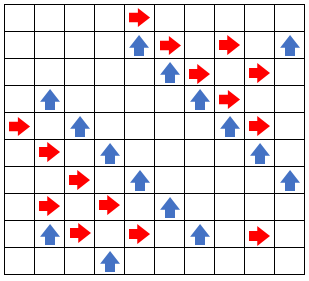
\includegraphics[width=0.4\textwidth]{ca1.PNG}\label{fig:ca1}}
  	\hfill
  	\subfloat[Jammed State]{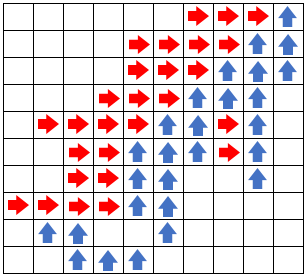
\includegraphics[width=0.4\textwidth]{ca2.PNG}\label{fig:ca2}}
  	\caption{Two states in the BML model. The red arrows are for eastward vehicles, while the blue arrows denote northward vehicles.}
\end{figure}


However, \shortciteA{M-BML:2016} modified the BML in such a way that it improved its performance. While the BML distributed the number of vehicles in eastwards and northwards equally, the M-BML distributed at random to be more realistic. In addition, current urban networks can be mapped immediately into the M-BML model for predicting traffic congestion.

% Knowledge-based
\shortciteA{Lee:KnowledgeBase}, meanwhile, developed a knowledge-based real-time travel time prediction model that uses location-based services (LBS) collected through data mining technologies. These LBS are collected from vehicles equipped with GPS and mobile data communication module to report its current speed, traveling direction and its current position. It also uses intersection delay patterns, discovered through sequential pattern mining, which is used to estimate the time to turn to an intersection. The model makes use of a dynamic linear combination of two weight predictors: the historical predictor and real-time predictor. Historical predictors are based on historical traffic information. It is used to estimate link travel time and predict intersection delays. On the other hand, the current predictor is based on real-time traffic information. It is used to incorporate external events into the travel time prediction of the model. The concept of dynamic linear combination allows the model to shift between these predictors. For instance, in the case of an external event (e.g. car accident), the model will reduce the weight of the historical predictor because the current predictor may be more reliable since the effect of this incident will immediately affect the traffic condition.

% H-ARIMA
The H-ARIMA model, on the other hand, makes use of 2 different submodels: ARIMA and HAM \shortcite{pan2012utilizing}. The ARIMA is an autoregressive moving average model that heavily relies on the combination of previous data collected just before the current time in determining the traffic condition for the next time series. Because it considers recent instances, the ARIMA is more optimal to use for short-term prediction. The HAM, on the other hand, relies more on the average of the previous data given that the data is on the same day of the week and at the same time of the day. In order to distinguish the most suitable approach for a given situation, The researchers trained a decision tree that selects which approach to use. Once given an input, the H-ARIMA feeds the input to both approaches and then gets the overall rate of the prediction error of both approaches. The overall rate of the prediction error is computed as the prediction error of the ARIMA divided by the sum of prediction errors of both approaches. If for instance, the rate of the ARIMA is less than the set threshold (0.5), it means that the ARIMA is to be used for the given situation.

% ANN AND SWT-ACNN
\shortciteA{Saputri2013} believed, however, that using ANN is the best method of forecasting amongst all others. Inspired by the nonlinear characteristics of Biological Brain System, the work performance of ANN can be compared to the workings of the human brain system. Besides its simple computation and fast performance, \shortciteA{ANN:2016} concluded that ANNs minimize the error in limited time; hence, it improves the efficiency and accuracy of the system. 

There were two models that used ANNs in their approach. One of them developed a traffic model that uses Jordan’s Sequential Neural Network, which has a good ability of generalization \shortcite{ANN:2016}. The structure of this kind of ANN is such that the distribution of nodes in the hidden layer should be the square of the number of nodes in the input layer. For example, if there are 5 nodes found in the input layer, then there must be 25 nodes in the hidden layer. The Jordan’s Neural Network contains four layers: (a) context layer, which acts as a memory and stores previous information, (b) input layer, which constitutes the input for the next processing, (c) hidden layer, which gets input from the “true” input layer and the context layer, and (d) output layer, which outputs the result or feedbacks to the context layer to be processed again. \figref{fig:annJordan} shows a Jordan’s Sequential Neural Network with 5 inputs in the input layer.

\begin{figure}[!t]
	\centering
	\captionsetup{justification=centering}
	\scalebox{.25}{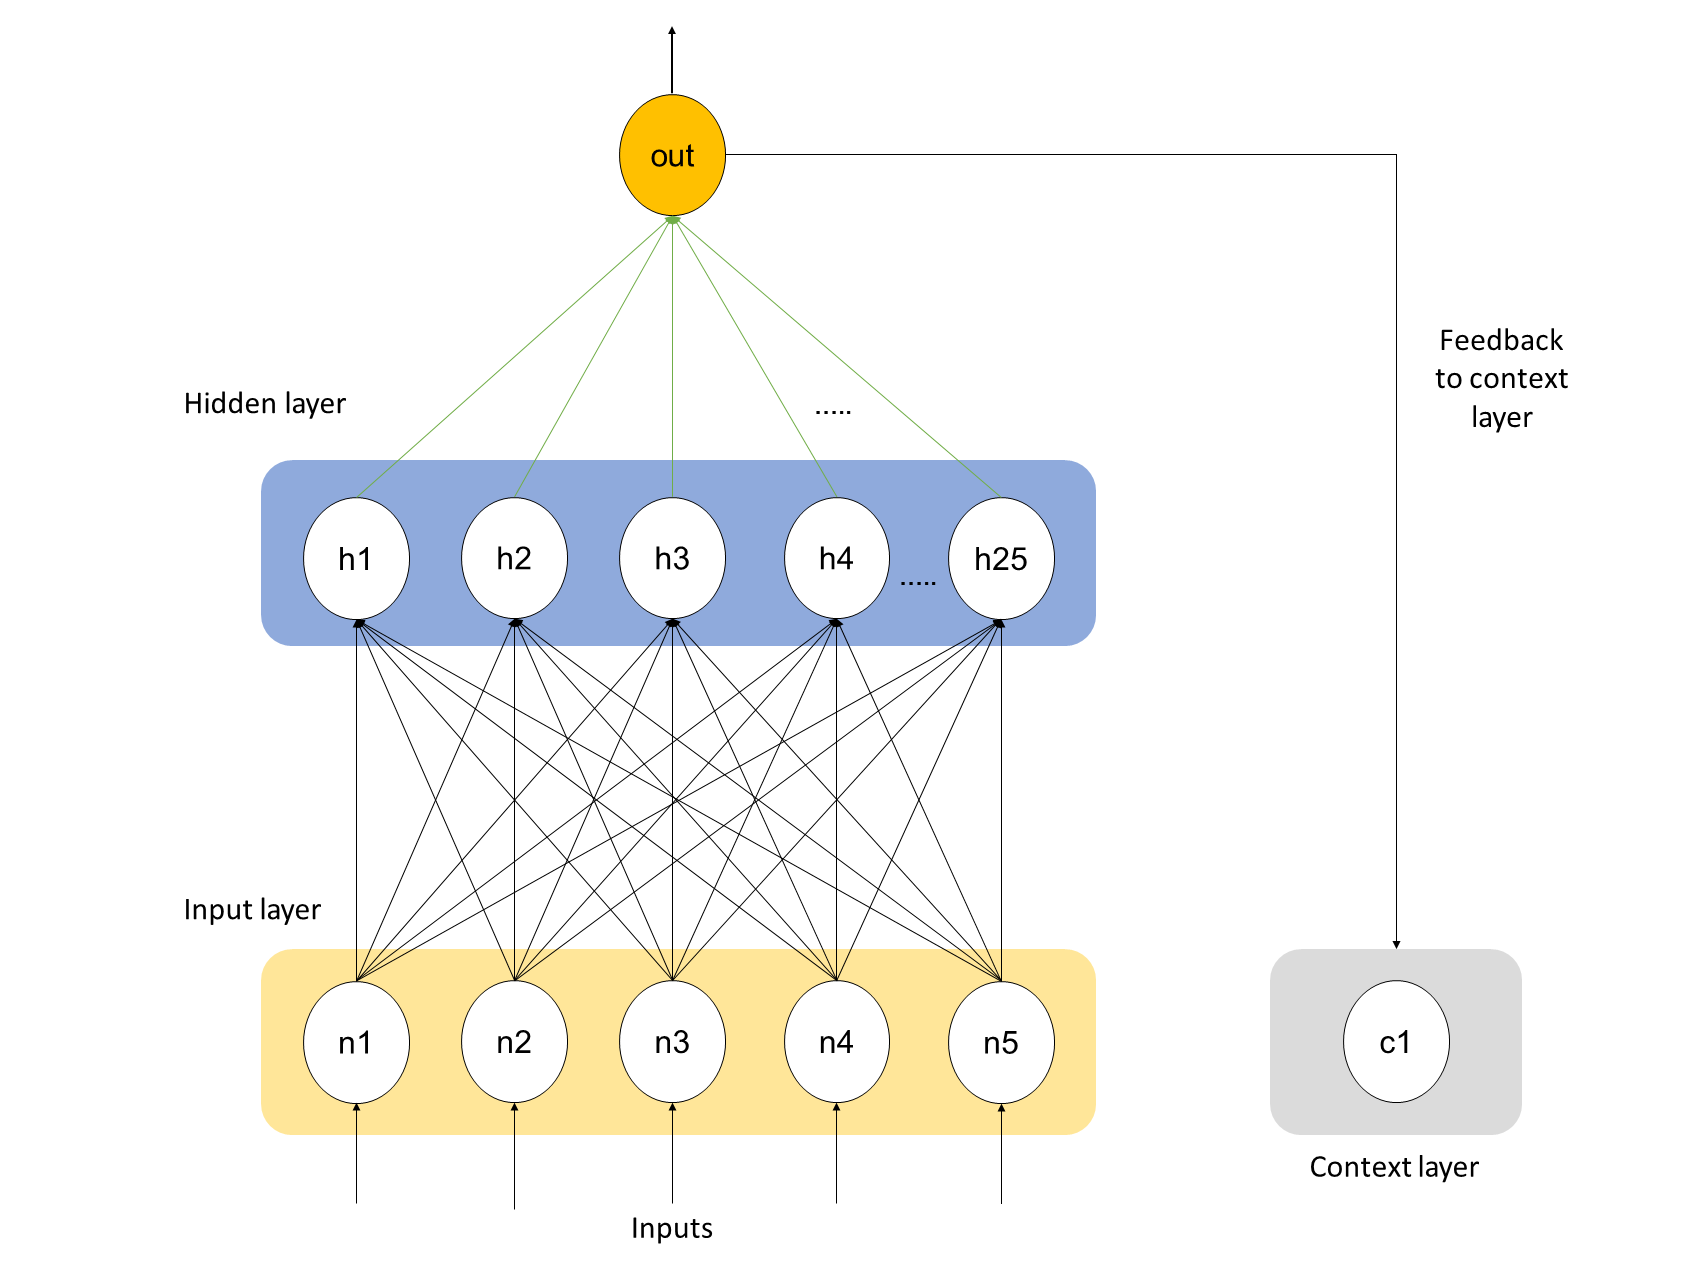
\includegraphics{ann.png}}
	\caption{ANN Framework used in More et al., 2016}
	\label{fig:annJordan}
\end{figure}

The ANN algorithm in the SWT + ACNN model, on the other hand, uses the structure of FeedForward (FF) Back Propagation (BP) algorithm for training \shortcite{dunne:2013}. The FF phase receives the input and passes it to the output layer through the hidden layer. As discussed earlier, the input fed into the neural network of the SWT + ACNN model is generated from auto-correlation. The output values are calculated from the input layer passing through the hidden layer, and is summed with the weights of the neural network units through activation functions. The BP phase compares the generated to the desired value. This phase optimizes the error function through a number of iterations until the error function is close to optimal. The ANN used by the SWT + ACNN, which takes in auto-correlated inputs, have been labeled as the Auto-Correlation Neural Network (ACNN).

% DBN with Data Fusion
In the developed model of \shortciteA{koesdwiady:2016}, Deep Belief Network (DBN) and data fusion techniques are used to enhance the generated prediction. DBN, unlike ANN, is composed of multiple layers of hidden units. The DBN of this model makes use of Restricted Boltzmann Machines (RBM), and stacks RBM together within the hidden layer. RBM is an unsupervised learning algorithm that can learn useful features of the data. It takes the input and translates them into a set of numbers that represents them. Then, these numbers can be translated back to reconstruct the inputs. This neural network is trained through multi-task learning to predict several traffic flow predictions at each level at the same time to reach the final traffic flow prediction. \shortciteA{koesdwiady:2016} further discusses that the optimal architecture for the DBN in traffic prediction consists of three hidden layers with 250 in the first, 200 in the second, and 100 in the last hidden layer. Additionally, \shortciteA{koesdwiady:2016} adds that 100 epochs is optimal for training the DBN. The separately predicted traffic flow and weather data will be fused using data fusion techniques to generate an enhanced and accurate traffic flow prediction. The DBN with Data Fusion makes use of Decision In - Decision Out (DEI-DEO) which fuses input data considered as the decision to generate a new or enhanced decision \shortcite{koesdwiady:2016}.

% RNN using LSTM
\shortciteA{Jia:2017} used RNN using LSTM to capture time series characteristics during its training and prediction phases. RNN uses memory cells to save information from previous time intervals. LSTM can adjust its hyperparameters to automatically adjust its hyperparameters from the data. The LSTM model consist of one input layer, one hidden layer, and one output layer. The hidden layer performs as the network's memory block that memorizes the long and short term temporal features. 

% MLRA
\shortciteA{Lee2015}, on the contrary, suggested a traffic model that makes use of multiple linear regression analysis (MLRA) employing both weather forecast data and traffic congestion data. MLR analysis is used to explain the relationship between one continuous dependent variable (traffic congestion data) and two or more independent variables (weather data). In this model, the traffic congestion is influenced by 48 independent variables. However, in their research, some of those independent variables are highly correlated to each other, and therefore should be removed to prevent the increase of correlation. 






\section{Evaluation Strategy}
Before computing the accuracy of each traffic models, different experiments and case studies were first performed. All traffic models were tested to predict the traffic congestion at a given time period.

% knowledge-based
In evaluating the knowledge-based model, \shortcite{Lee:KnowledgeBase} collected five months of location-based service (LBS) raw data. The LBS raw data was collected through an online taxi dispatch system (TDS), consisting of around 500 taxis operating 24-7 in a Taipei urban area. The first four months are used for mining traffic patterns, whereas the fifth is used for verifying the accuracy of the model. In the experiment, a random origin-destination pair is selected at two peak hour sections. The model produced a precision of 10.8\% \textit{relative mean error} (RME) and \textit{root mean squared error} RMSE of 15.92\%. To further challenge its reliability, the experiment was performed with the same set of input, having the intersection delay replaced with a turning delay estimate from a human expert. The model produced a precision of 20\% RME and 30.55\% RMSE, which, in comparison with the pattern generated intersection delay, is relatively unreliable. 

% H-ARIMA
In evaluating the accuracy of the H-ARIMA model, the researchers compared results with other baseline approaches given two situations: short-term prediction and long-term prediction \shortcite{pan2012utilizing}. RMSE and \textit{mean absolute percentage error} (MAPE) were used to measure the accuracy of the traffic prediction. Although the H-ARIMA model was able to yield better results than the other baseline approaches for short-term prediction, the researchers were not able to see the edge of the H-ARIMA model against them. Similar to that, the H-ARIMA model was also able to produce a better result for long-term prediction compared to the baseline approaches. It was observed that its MAPE is lower compared to others because it considers historical traffic data in predicting traffic. Overall, the H-ARIMA model was able to produce around 95-96\% accuracy.

% DBN with Data Fusion
To measure the accuracy of the predictions of the DBN with Data Fusion, performance indexes RMSE and MAE are used \shortcite{koesdwiady:2016}. These performance indices calculate the error value of the prediction by comparing the actual and predicted output at a certain time \textit{t}. The research compared the performance of different neural networks of ARIMA and ANN with DBN. After experimentation, the DBN outperformed the other neural networks in predicting traffic flow. The performance of the DBN generated an average MAE of 0.07 and average RMSE of 0.05. On the other hand, ANN generated an average MAE of 0.08, and an average of RMSE of 0.06, and ARIMA generated an average MAE of 0.27 and an average RMSE of 0.23.

To examine the performance of the neural network with low, medium and heavy traffic, three different freeways that experience the mentioned traffic conditions are chosen \shortcite{koesdwiady:2016}. The detrended version of the data was more accurate in predicting heavy traffic, and the original data was more accurate in predicting low and medium traffic. Medium traffic flow using original data achieved an MAE of 0.041 and RMSE of 0.06. Low traffic flow using original data achieved MAE of 0.034 and RMSE of 0.045.On the other hand, detrended version of the data performed best in predicting high traffic flow achieving an MAE of 0.06 and RMSE of 0.09. Moreover, using weekday/weekend version of the data generated a higher average error. Furthermore, the model better predicts the medium traffic flow with consideration to weather information.

For \shortciteA{Jia:2017}, they evaluated the model, and its effectiveness in predicting traffic with consideration of rainfall, through comparing the performances of DBN and LSTM models with and without rainfall consideration. The test dataset used for evaluating consist of instances when rainfall was significantly present. The study used MAE, MAPE and RMSE as the evaluation metrics. Results show that predicting 10-minute traffic volume is more accurate than predicting a 30-minute traffic volume. Moreover, the LSTM model performed better than DBN with or without considering rainfall, showing the advantage of LSTM to capture time series patterns of the traffic data. The LSTM model achieved an RMSE (vel/h) of 240.98 and  269.91 for the 10-minute and 30-minute prediction, respectively, while the DBN model achieved an RMSE (vel/h) of 255.79 and 365.49, showing a significant change from the performance of LSTM. 

% SWT-ACNN
The model’s performance was compared to ANN that takes in undecomposed data to observe the differences in performance. To measure the accuracy and performance, RMSE and MAPE were used. The SWT-ACNN outperformed the non-wavelet model significantly by approximately 5\% of MAPE, and 40 of RMSE. Additionally, the wet model is superior to the dry model achieving a MAPE of more than 30\% than the dry model.

To compare the results of \shortciteA{Lee2015}’s MLRA model with the actual values, present traffic congestion data were used. As discussed in the previous section, the weather data used in their research are temperature, humidity, rainfall. In their analysis, they used MAPE to assess the developed MLRA model. When they predicted the traffic congestion from July and August 2013, the traffic model got an accuracy of 94.1\%. However, when they predicted the traffic congestion in 2014 for the same months, they have arrived at 84.8\%. %This may be because the weather and traffic congestion data used to create this model came from July and August 2013.




\begin{sidewaystable}
	\caption{Summary of Traffic Models}
    \centering
    \begin{tabular}{| L{3cm} | L{3cm} | L{3cm} | L{3cm} | L{3cm} | L{3cm} | L{2cm} |} 
    
    \hline
    Author (Year) & Modeling Approach & Traffic Data Input & Weather Data Input & Coverage & Evaluation Strategy & Accuracy \\
    
    \hline
    \shortciteA{M-BML:2016} &
    Cellular Automata (CA)  &
    - traffic density \newline - evolution rules &  
    none & 
    - road segment \newline - Birmingham, England & 
    not indicated &
    94.00\% \\
    
    \hline
    \shortciteA{ANN:2016} &
    Artificial Neural Network (ANN) &
    traffic volume &
    none &
    - road segment \newline - Dublin, Ireland & 
    not indicated &
    92.00 - 98.00\% \\
    
    \hline
    \shortciteA{Lee:KnowledgeBase} &
    Knowledge-based &
    - vehicle GPS data
    \newline
	- intersection delay & 
    none &
    - whole city
    \newline
	- Taipei, Taiwan &
    - RMSE
    \newline
    - RME
    &
    84.08\% \\

	\hline
    \shortcite{pan2012utilizing} & 
    HAM and ARIMA (H-ARIMA) &
    - traffic volume
    \newline
	- speed &
    none &
    - road segment
    \newline
	- Los Angeles, USA &
    - RMSE
    \newline
    - MAPE
    &
    95.99\% \\

	\hline
    \shortciteA{koesdwiady:2016} &
    Deep Belief Network with Data Fusion (DBN with Data Fusion) &
    - traffic volume &
    - temperature
    \newline
    - wind gust
    \newline
    - weather condition &
    - road segment
    \newline
    - San Francisco, USA &
    - RMSE
    \newline
    - MAE
    &
    95.95\% \\
    
    \hline
    \shortciteA{dunne:2013} &
    Stationary Wavelet Transform and Auto-Correlation Neural Networks (SWT-ACNN) &
    - traffic volume &
    - rainfall &
    - road segment
    \newline
    - Dublin, Ireland & 
    - RMSE
    \newline
    - MAPE
    &
    91.45\% \\
    
    \hline
    \shortciteA{Lee2015} &
    Multiple Linear Regression Analysis (MLRA) &
    - speed 
    \newline
    - travel time
    \newline
    - traffic volume &
    - temperature &
    - whole city 
    \newline
    Seoul, South Korea &
    - MAPE &
    84.80\% \\
    
    \hline
    
    \end{tabular}
\end{sidewaystable}
               %-- includes LaTeX source file for Chapter 2: Review of Related Literature
                                  %-- your job: **EDIT THIS FILE** to indicate your review of related literature 

\chapter{Theoretical Framework}
\label{theoframework}




\section{Traffic-related terms}
\subsubsection{Traffic flow}
According to \shortciteA{may1990}, traffic flow studies how travelers interact with infrastructures and with each other, in order to understand the movement of traffic and how can it be improved with less congestion. These travelers include drivers, pedestrians, among others, while infrastructures include roads, signages, stop lights, and other devices that control traffic.

\subsubsection{Traffic speed}
The speed of a vehicle can be computed by measuring the distance it traveled per unit time. Because the speed of each vehicle may be different from its neighboring vehicles, traffic speed is the average of the speed of each vehicle in the given environment. 

\subsubsection{Traffic volume}
Traffic volume refers to the number of vehicles present in a certain road at a given time.

\subsubsection{Traffic density}
Given a length of a road, traffic density is measured by the number of vehicles present. This means that if the traffic density is low, then there is no traffic congestion because the vehicles are apart from each other. In reverse, if the traffic density is high, then the vehicles are close to each other; thus, a traffic congestion.

\subsubsection{Traffic condition}
Traffic conditions refer to the states of traffic at a certain point at a certain time, with respect to traffic flow, speed, volume, and density. It has three major states: light, moderate, and heavy traffic.

\subsection{Traffic Congestion}
Traffic congestion, according to \shortcite{vuchic1994bus}, happens when traffic volume on a particular road goes beyond the road’s capacity. \shortcite{bovy2002congestion} define traffic congestion as the state of traffic flow on a particular road with low speeds and high densities compared to some other state with high speeds and low densities. 

\subsubsection{Road and road segments}
A road is a wide path from one place to another, usually paved for the vehicles to drive on \shortcite{wang2013}. Typically, a road is created for vehicles to head two opposite directions, northbound and southbound. A road segment, on the other hand, is a portion of a road heading in one direction, separated by infrastructures (e.g. train stations, landmarks, intersections).




\section{Weather-related terms}

\subsubsection{Temperature}
Temperature is the measure of the hotness and the coldness of an object. There are three major scales that are being used internationally, \textit{Celsius}, \textit{Fahrenheit}, and \textit{Kelvin}. 

\subsubsection{Dew point}
Dew point is the temperature wherein moisture or \textit{dew} appears on solid surfaces. This is caused by condensation, in which the water vaporizes into its liquid form at certain amounts of pressure. 

\subsubsection{Humidity}
Humidity refers to the quantity of the water vapor contained in the air. Measured in percentage, relative humidity, on the other hand, is the quantity of water vapor in relation to how much the air can hold at a certain temperature. If the air is warm, it has high relative humidity since the air holds more water vapor than cold air. 

\subsubsection{Wind speed}
Wind speed is the average wind speed in the indicated amount of time. Because of the changing temperature, wind speed results from the air going from above average temperature to a lower temperature. 

\subsubsection{Wind Gust}
Wind gust is the short, rapid rise of wind speed before quickly calming. The wind is forced to change its direction and speed quickly because of sudden decrease in temperature,  wind shears, and friction.

\subsubsection{Precipitation}
Precipitation refers to any result of air condensation that falls due to the pull of gravity. This includes, but not limited to, rain, snow, and hail. Usually, precipitation is measured in terms of millimeters (mm).

\subsubsection{Visibility}
Visibility is the measure of how long can we distinguish light or an object at a certain distance.  

\subsubsection{Pressure}
Pressure, also called atmospheric pressure, is the amount of force exerted by the air molecules in a particular surface area of the earth. Meteorologists use millibars (mb) to measure pressure. 

\subsubsection{Cloud Cover}
Cloud cover is defined as the amount of clouds in a fragment of the sky in a particular location. This contributes to the weather condition and visibility. This is usually measured by \textit{okta}.

\subsubsection{Heat Index}
Heat index is the temperature of how hot the human body feels like. This is directly related to air temperature and relative humidity. 

\subsubsection{Feels-like}
Feels-like is the temperature of how cold the human body feels like when the wind touches the skin.




\section{Historical Data}
Historical data is an extensive archive of data that can be utilized to detect regularities or pattern for predicting future outcomes. It ranges from months-worth to years-worth of past data. The following section features sources whose historical data will be used for the research.

\subsection{Traffic Data from MMDA’s Traffic Monitoring System}
The traffic dataset includes traffic conditions for nine major roads in Metro Manila, collected in a 15 minute time interval. The traffic condition can either be \textit{light} (L), \textit{moderate} (M), or \textit{heavy} (H). However, if no information is available, it can also appear as \textit{none} (N).

Major roads from this dataset include EDSA, Commonwealth, Quezon Avenue, España, C5, Ortigas, Marcos Highway, Roxas Boulevard, and SLEX. Each road consists of a number road segments, which includes a northbound lane and a southbound lane. For instance, EDSA consists of 37 road segments (e.g. Balintawak, Kaingin Road, Muñoz).

Table \ref{table:sample_traffic_data} shows a sample raw data collected from MMDA’s traffic monitoring system. From the sample data, it can be observed that despite not having a traffic condition entry, the interval is still being recorded as part of the dataset, having a traffic condition record of \textit{none} (N).

\begin{table}[h]
	\centering
    \footnotesize
	\caption{Sample of Traffic Data from MMDA's Traffic Monitoring System}
	\label{table:sample_traffic_data}
	\begin{tabular}{|l|l|l|p{2.5cm}|p{2.5cm}|}
		\hline
		Date and Time & Road & Segment & Condition (Northbound) & Condition (Southbound) \\ \hline
		2015-01-01 00:00:00 & EDSA & Quezon Ave. & L & L \\ \hline
		2015-01-01 00:00:00 & EDSA & Taft Ave.& M & M  \\ \hline
		2015-01-01 00:00:00 & ESPAÑA & Welcome Rotunda& L & L  \\ \hline
		2015-01-01 00:15:00 & EDSA & Quezon Ave.& N & N  \\ \hline
		2015-01-01 00:15:00 & EDSA & Taft Ave.& M & M  \\ \hline
		2015-01-01 00:15:00 & ESPAÑA & Welcome Rotunda& L & L  \\ \hline
	\end{tabular}
\end{table}


\subsection{Weather Data from World Weather Online}
The weather dataset from World Weather Online includes temperature (in both Celsius and Fahrenheit), humidity (in percentage), pressure (in millibars), wind speed (in both miles per hour and kilometers per hour), and dew point (in both Celsius and Fahrenheit), cloud cover amount (in percentage), heat index (in both Celsius and Fahrenheit), visibility (in kilometers), wind chill temperature (in both Celsius and Fahrenheit), wind gust (in both miles per hour and kilometers per hour), feels-like temperature (in both Celsius and Fahrenheit), and precipitation (in millimeters). This data is sampled every one hour of every day and is a generalized reading for the whole city of Manila.

Table \ref{table:sample_worldweatheronline_weather_data} shows a sample raw data collected from World Weather Online. It could be observed that the conversion of some variables to different units has already been performed as part of the data. Furthermore, missing data is not evident from the samples collected.


\begin{table}[h]
	\centering
	\caption{Sample of Weather Data from World Weather Online}
	\label{table:sample_worldweatheronline_weather_data}
	\begin{tabular}{|l|r|}
		\hline
          Property & Sample Value \\ \hline
          Date & 2015-10-01 \\ \hline
          Time & 0 \\ \hline
          Weather Condition & Moderate or heavy rain shower \\ \hline
          Temperature (\textdegree{}C) & 27 \\ \hline
          Temperature (\textdegree{}F) & 81 \\ \hline
          Wind Speed (m/h) & 2 \\ \hline
          Wind Speed (km/h) & 4 \\ \hline
          Humidity (\%) & 87 \\ \hline
          Visibility (km) & 8 \\ \hline
          Pressure (mb) & 1013 \\ \hline
          Cloud Cover (\%) & 27 \\ \hline
          Heat Index (\textdegree{}C) & 31 \\ \hline
          Heat Index (\textdegree{}F) & 88 \\ \hline
          Dew Point (\textdegree{}C) & 25 \\ \hline
          Dew Point (\textdegree{}F) & 76 \\ \hline
          Wind Chill (\textdegree{}C) & 27 \\ \hline
          Wind Chill (\textdegree{}F) & 81 \\ \hline
          Wind Gust (m/h) & 4 \\ \hline
          Wind Gust (km/h) & 7 \\ \hline
          Feels Like (\textdegree{}C) & 31 \\ \hline
          Feels Like (\textdegree{}F) & 88 \\ \hline
          Precipitation (mm) & 2.8 \\ \hline
	\end{tabular}
\end{table}



\section{Working Day}
A working day refers to a day in which people are assigned on duty in an organization (e.g. company, government, school, etc.) each week \cite{liu2008wdcm}. For most organizations, working day is defined to be from Mondays to Fridays. Non-working days, meanwhile, are from Saturdays to Sundays. As people are on duty during working days, this implies an increase in demand on transportation when going to their respective organizations \shortcite{traffic_trend}. Thus, there is an increase in traffic volume due to the demand during weekdays as compared to weekends.

Aside from weekends, there are also instances in which a weekday can be classified as a non-working day. This occurs during holidays or whenever a public-sector or government announces class or work suspension.



\section{Peak Hour}
A peak hour, or rush hour, is a time of the day where the congestion of traffic in roads or inflation of people in public transports are at its highest peak \shortcite{downs2005still}. There are two peak hours each weekday: the morning peak hour and the afternoon or evening peak hour. These are the times when majority of the people travel and commute to go to work or school. The morning peak hours depict the time when employees and students travel towards their workplace or school, while the evening peak hours suggest the time when they return to their respective homes. These periods may last for more than one hour, and may vary from road to road, city to city, country to country, and seasonally. 


\section{Weather Disruptions}
Weather disruptions such as typhoons and low-pressure areas have brought heavy and prolonged precipitation which often causes flooding in some areas. One example of these extreme weather disruptions is Typhoon Goring that occurred from July 22, 2015 until July 26, 2015. Weather disruptions typically produce a significant amount of precipitation in just one day. These prolonged rain periods usually last for days, thus building up the effects it brings as time goes by.





\section{Traffic Model}
% definition of traffic model
Mathematically, a traffic model is a representation of traffic in the real-world \shortcite{mahmud2016}. These models exist to help researchers understand how traffic works and how can the congestions be minimized by simulating them in a way that researchers can explore and manipulate. 

% macroscopic and microscopic model
There are two major types of traffic models: \textit{macroscopic} and \textit{microscopic} traffic models \shortcite{mahmud2016}. A macroscopic traffic model deals with the properties of transportation elements in the bigger picture. It describes the circulation of traffic without going into its individual components. Macroscopic traffic models usually describe traffic using flow-rate, volume, density, speed, among others. A microscopic traffic model, on the other hand, deals with characteristics of the individual transportation elements. This covers driver behavior, how the vehicles move, element interaction, among others. These kinds of traffic models use various learning algorithms like regression, neural networks, clustering, decision trees, among others. 




\section{Linear Interpolation}
Using surrounding data points, interpolation can be used to determine the value of an unknown point in a line. Linear interpolation is one method of interpolation where it assumes a linear or straight line relationship between two known points. It is used to approximate value through the weighted average of two points. The equation for Linear Interpolation is defined as:

\begin {equation}
y = y_1 + \frac{y_2 - y_1}{x_2 - x_1} (x - x_1)
\end{equation}



\section{Correlation}
% Spearman’s rank correlation coefficient
The Spearman`s rank correlation coefficient is an approach for statistical dependence between two independent variables while not consider the parameters of a frequency distribution (nonparametric) \shortcite{Zar1972SignificanceCoefficient, Liu2010ARecognition, Gauthier2001DetectingCoefficient}. The rank correlation coefficient, $r_s$, can be expressed using a monotonic function as: 

\begin {equation}
r_s = 1 - \frac{6 \sum a^2}{N(N^2 - 1)}
\end{equation}

\noindent where $r_s$  represents the Spearman’s rank correlation coefficient, $a$ denotes the ranked difference between the $i$th measurements for the two random variables, and $N$ is the number of measurements in each of the two random variables in the correlation \shortcite{Zar1972SignificanceCoefficient}. Spearman’s $r_s$ measures the strength and course of the \textit{monotonic} relationship between ranked variables. \shortciteA{Hauke2011ComparisonData}, meanwhile, explain that Spearman’s $r_s$ can be considered as the correlation coefficient of Pearson that deals with ranks.  

% Pearson’s product moment correlation coefficient
Pearson`s product moment correlation coefficient, commonly Pearson’s correlation coefficient or Pearson’s r, is the most commonly used correlation statistic to measure the strength and course of the \textit{linear} relationship between two continuous variables \shortcite{ahlgren2003}. It is expressed using this function:

\begin {equation}
r = \frac{\sum (A - \bar{A})(B - \bar{B})}{\sqrt[]{\sum (A - \bar{A})^2 \sum(B - \bar{B})^2}}
\end{equation}

\noindent where $r$ represents the Pearson’s r, $A$ and $B$ denote the two variables being observed, and $\bar{A}$ and $\bar{B}$ are the averages of the two variables respectively. 

% Results of Pearson and Spearman
Both correlation analysis outputs a value between -1 to +1. If the result of a correlation is close to +1, then variable A has a positive relationship with variable B; vice versa, if the result is close to -1, then variable A has a negative relationship with variable B. If the result is approaching 0, then variable A has no relationship with variable B. Table \ref{table:correlation-results} shows the correlation relationships with their corresponding ranges, where $x$ is the exact correlation result. 


\begin{table}[h]
\centering
\caption{Results of Pearson and Spearman}
\label{table:correlation-results}
\begin{tabular}{|l|r|}
\hline
Correlation Relationship         & \multicolumn{1}{l|}{Value}        \\ \hline
very strong positive correlation & 0.9 $<$ x $\leq$ 1.0   \\ \hline
strong positive correlation      & 0.7 $<$ x $\leq$ 0.9   \\ \hline
moderate positive correlation    & 0.5 $<$ x $\leq$ 0.9   \\ \hline
low positive correlation         & 0.3 $<$ x $\leq$ 0.5   \\ \hline
no correlation                   & -0.3 $<$ x $\leq$ 0.3  \\ \hline
low negative correlation         & -0.5 $<$ x $\leq$ -0.3 \\ \hline
moderate negative correlation    & -0.7 $<$ x $\leq$ -0.5 \\ \hline
strong negative correlation      & -0.9 $<$ x $\leq$ -0.7 \\ \hline
very strong positive correlation & -1.0 $<$ x $\leq$ -0.9 \\ \hline
\end{tabular}
\end{table}

% Advantage of Spearman over Pearson
Although Spearman is considered a Pearson’s r measure in terms of ranks, there are advantages that enable Spearman to be a more powerful measurement over Pearson \shortcite{Gauthier2001DetectingCoefficient}. Spearman’s rank correlation coefficient is not affected by the distribution of the values, unlike Pearson’s r, which normal distribution is analyzed. Furthermore, instead of the raw data, it does not care for outliers because it deals with the ranks of the data. In addition, the data does not need to be in time-series, where the intervals are regular. In contrast, since Spearman disregards the outliers when it turns the data into ranks, there is a loss of information. Moreover, it is less powerful than the Pearson’s r if the data is normally distributed.


\subsubsection{Seasonality}
Seasonality refers to the characteristic of a time series in which the data experiences regular and predictable changes that recur every number of intervals. In trend analysis, determining the data`s seasonality is significant as it could define a "normal pattern" by getting the mean of several samples per seasonal interval.


\subsubsection{Autocorrelation}
Autocorrelation, sometimes called \textit{serial correlation} or \textit{lagged correlation}, measures the similarity or correlation of an observation in a time series and itself shifted in a specific time \textit{lag}. The series of numbers arranged in time is correlated to the values of its own past and future. The purpose of autocorrelation is to find out if there is a pattern repeating in the data. The formula for autocorrelation is as follows: 

\begin{equation}
r_{k} = \frac{\sum_{i=1}^{N-k}(X_{i} - \bar{X})(X_{i+k} - \bar{X})} {\sum_{i=1}^{N}(X_{i} - \bar{X})^{2} }
\end{equation}

\noindent where $k$ denotes the lags and $N$ as the number of observations in the series.


\subsubsection{Lag}
Lag refers to the amount of delay between a given observation. For instance, a comparison between Tuesday`s 12 PM and the last week`s Tuesday`s 12 PM is incidated as a one day lag.


 \subsubsection{Autocorrelation plot}
Autocorrelation plot is a collection of autocorrelation coefficient values from a range of time lags. It is commonly used for evaluating the randomness of the dataset. It can be used to measure seasonality as it reveals how many intervals does it take for the pattern to reappear.

It consists of three parts: the y-axis, the x-axis, and the reference lines. The y-axis consists of correlation coefficient values, while the x-axis consists of time lags defined as \textit{t} where \textit{t = {1, 2, 3, ..., n-1, n}}.

\section{Feature Engineering}
Feature engineering is important for any system that uses machine learning. The performance of machine learning algorithms depends on how the data was presented to them. If they accept raw data directly, they would not give the intended results since machine learning algorithms do not have the capacity to extract insightful features from raw data automatically. This is where feature engineering comes in. It is using the domain knowledge of and from the raw data and create insightful features which would help machine learning algorithms to perform better. 

A feature is a property that is common with all the independent units in the raw data. Choosing the right features for the model is of utmost necessity. To yield better results, models should be simple and be more flexible, which better features would produce.

The process of feature engineering is difficult and exhaustive. At first, a lot of features need to be decided and created regardless of its relevance. Afterwards, these features would be checked with the model to identify how and which features would help the model. Then, to avoid overfitting, feature selection should be used. This process would repeat until certain features are finalized and used with the model. The steps to follow look like this:

\begin{enumerate}
     \item Brainstorm features. Understand the problem, explore the data, and find studies that are similar to your problem and how they used feature engineering to solve their problem.
     \item Devise features. Decide on what features to create based on the problem at hand.
     \item Create features. Use different feature selection methods and feature importance scorings to create feautes.
     \item Test features with the model. Estimate the accuracy of the model on unseen data using the chosen features.
     \item Improve features. Modify the features depending on the result of the model's accuracy.
     \item Repeat Step 1 until the work is done.
\end{enumerate}





\section{Fusion Techniques}
To achieve the best performance, fusion techniques were made for designing systems which recognize patterns. By combining data, features, or decisions from a set of sensors, better inferences are made and accuracy is improved \shortcite{sohn2003}. Fusion techniques are applied in the field of military, where targets are automatically recognized \shortcite{bosse2006}, in the field of image processing for medicine \shortcite{constantinidis2001}, face recognition \shortcite{mangai2010}, robotics \shortcite{jimenez1999}, among others. There are three levels for fusion techniques: \textit{data fusion, feature fusion, } and \textit{decision fusion}. In this paper, only the feature fusion and decision fusion will be discussed. In addition, there are numerous techniques to solve fusion problems, but in this paper, only neural networks and weighted average will be discussed.

\subsection{Fusion Levels}
\subsubsection{Feature Fusion}
Features are the most essential information needed to accomplish any classification task. Although important, not all features contribute to the performance of a classifier. Features that do not match the rest of the dataset can have an effect to the pattern recognized by the classifier. Thus, they should be removed from the dataset \shortcite{mangai2010}. The process of improving or obtaining new features is called feature fusion \shortcite{castanedo2013}. 

\shortciteA{Dasarathy1997SensorApplications} broke down the common hierarchy of fusion into five levels. In the said breakdown, he defined feature fusion as the Feature In- Feature Out Fusion (FEI-FEO). This fusion process accepts and outputs features. Feature fusion can be divided into three methods:  feature ranking and selection, feature extraction, and combination \shortcite{mangai2010}.

\shortciteA{mangai2010} described feature ranking and selection as the soul of feature fusion. It aims to find the optimal subset that can represent the entire dataset. In feature extraction, on the other hand, features are reduced and ranked for a better analysis \shortciteA{Dasarathy1997SensorApplications}. Lastly, feature combination derives new features from at least two selected features.

Another fusion level that accepts features is the Feature In-Decision Out Fusion (FEI-DEO). Its difference with the FEI-FEO Fusion is that instead of having features as its output, it outputs a decision instead. Some researchers refer to this as either feature fusion because of its input or decision fusion because it outputs a decision. It all depends on the researcher’s view  \shortcite{Dasarathy1997SensorApplications}. It is commonly used by researchers for pattern recognition systems that generates a decision based on inputs from different sensors \shortcite{castanedo2013}.

With the issues involving the validity of decision fusion for the affective field, \shortciteA{dmello_graesser_2010} used feature fusion for a multimodal affect detection system. The researchers combined features to generate a better distinction between common human experiences such as confusion, frustration, engagement, delight, boredom, and neutral. They concatenated features from three sensory channels to produce a multichannel feature set. As a result, they were able to generate four multichannel models: Facial-Dialogue (FD) model, Facial-Posture (FP) model, Dialogue-Posture (DP) model, and Facial-Dialogue-Posture (FDP) model. They used feature selection to filter out a number of features that have the highest F-ratio. These features were then combined with the set of features selected from the other channel. 

\shortciteA{geetha_radhakrishnan_2013} were able to get satisfactory classification results after fusing fingerprint and palmprint features for a multimodal biometric authentication system. It aims to identify the set of most important features that can be used for a better recognition accuracy.The researchers claimed that fusing the features extracted from 2D Gabon  filter, stationary wavelet transform (SWT), and principal component analysis (PCA) by concatenation would result into a large feature set. This makes computing match scores more laborious. Hence, they used a wavelet-based fusion algorithm to fuse the extracted features. After using SWT to extract line information, the researchers used the mean-max fusion method to fuse the said features.

\subsubsection{Decision Fusion}
% definition
A decision is a conclusion stemmed from facts of a discerned events and activities \shortcite{castanedo2013}. As the high-level fusion technique, the decision fusion is more complicated since it inputs decisions from multiple classifiers to obtain one accurate decision \shortcite{mangai2010}. \shortciteA{Dasarathy1997SensorApplications} defines decision fusion as the Decision In - Decision Out (DEI-DEO) fusion in his five-step hierarchy of fusion based on input and outputs (see \figref{fig:dei-deo}). This combines multiple decisions from the input and outputs a more appropriate decision.


\begin{figure}[h]
	\centering
	\captionsetup{justification=centering}
	\scalebox{.50}{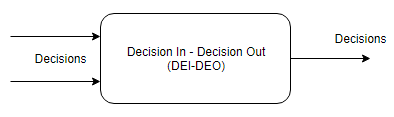
\includegraphics{dei_deo.PNG}}
	\caption{Dasarathy’s Decision In - Decision Out (DEI-DEO)}
	\label{fig:dei-deo}
\end{figure}

%advantages
\shortciteA{Dasarathy1997SensorApplications} also argues that while DEI-DEO fusion does not always trump data or feature fusion, the whole system does not fail if one of the sensors fail, unlike the other fusion techniques. He further explains that the DEI-DEO has less computational demands than the data or feature fusion, and that the bandwidth for communication is not important.

\shortciteA{castanedo2013} states one of the most used methods for decision fusion. The first method is the \textit{Bayesian Method}. This technique combines facts from probability theory rules, where the input and the outputs are probabilities in between [0, 1]. This method is derived from the Bayes rule: 

\begin{equation}
P(B | A) = \frac{P(A | B) P(B)}{P(A)},
\end{equation}

\noindent which gives us the probability of $B$ given $A$. However, because the probabilities $P(A | B)$ and $P(A)$ are not always known, it may not be applicable to some cases. Furthermore, \shortciteA{hall2001} state that the Bayesian method has a complexity problem if there are more than one possible result for $P(B | A)$. 

% applications
Other than Bayesian method, there are other techniques that can be applied to decision fusion, such as the Dempster-Shafer inference, abductive reasoning, semantic methods \shortcite{castanedo2013}, logistic function, weighted decision methods \shortcite{sohn2003}, projection pursuit, majority voting, fuzzy logic, and neural networks \shortcite{jimenez1999}. 


% \subsection{Fusion Algorithms}
% \subsubsection {Neural Networks}
% One of the techniques that can solve fusion problems is through neural networks \shortcite{fincher1990}. The advantage of having neural network as a technique for fusion over statistical approaches, such as Bayesian Method, is that it does not need to know certain probability errors beforehand. It can train itself with the current facts at hand and still get accurate results.  In the following papers, they used neural networks to fuse multiple sensors by recognizing the patterns given the inputs via their supervised training algorithm such as perceptron and backpropagation.
 
% \begin{figure}[h]
% 	\centering
% 	\captionsetup{justification=centering}
% 	\scalebox{.6}{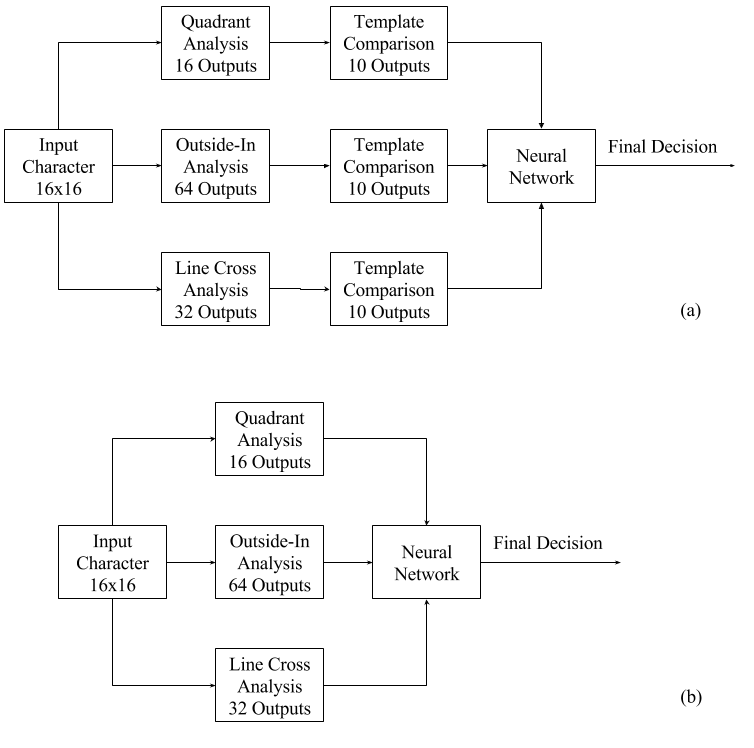
\includegraphics{fincher_approach.png}}
% 	\caption{(a) Structure of the Fincher’s Pre-Detection Approach, and (b) Structure of the Fincher’s Post Detection Approach}
% 	\label{fig:fincher_approach}
% \end{figure}

% In \shortciteA{fincher1990}, they used neural network-based data fusion for recognizing patterns between handwritten and computer-made numbers. The network is fed a 16 $\times$ 16 input character, and outputs the number recognized. They used two approaches in fusion: pre-detection and post-detection. In pre-detection, the input is fed into three algorithms: Quadrant Analysis, Outside-In Procedure, Line Cross Analysis. The outputs of these three algorithms are then compared to a template and creates decisions based from the algorithm outputs. These decisions are then fused through a neural network. In post-detection the outputs of the three algorithms are fed straight to the neural network to avoid loss of data. In this paper, pre-detection detected the correct pattern 93\% of the time than post-detection which detected the pattern 86\% of the time. The network bases its decision on the aspects of the input such as how close is one pixel to the other, and the importance of a value in a pixel. The network was trained through a supervised learning algorithm to merge and recognize the patterns based from the features of the input. The pre-detection follows the DEI-DEO fusion where the decision of the template comparisons are fused to generate the final decision, the pattern recognized from the inputs. On the other hand, the post-detection follows the FEI-DEO fusion where the input of the network is the features of the 16 x 16 input character and the output is the pattern recognized from the input. \figref{fig:fincher_approach} illustrates the pre-detection and post-detection approach.

% Likewise, in \shortciteA{dai1999}, they used neural networks for image processing to recognize changes between pictures of the same location of different times. The network is fed raw data from multiple sensors sequentially into 12 input layer units. Like \shortcite{fincher1990}, the network bases its decision from the inputs given. Additionally, the network’s hidden units play the role as the change extractor - one that can recognize and extract changes of the input and pass it to the next hidden layer. Finally, the network will output change map. 

% In \shortcite{jimenez1999}, they compared different methods of decision fusion (DEI-DEO), including multilayer neural networks, in hyperspectral imaging. In their architecture, the inputs for their neural network are the decision outputs from different classifiers, whose inputs are vectors of a spectral band in an image. The network was trained through Perceptron supervised training algorithm. Merging the inputs via supervised learning, their output is a single decision obtained from the training of the neural network, identifying the object in the image. 

% \subsubsection{Weighted Average}
% The Weighted Average is a signal-level fusion method that takes the weighted average of repeating information from the original inputs \shortcite{king2017, yan2011, meurant1992}. \shortciteA{king2017} claimed that using this method will ease the effect of unwanted data in the final estimation. This method can be used to estimate user activity details such as intensity, postures, and fundamental static for activity recognition systems. 

% \shortciteA{yan2011} proposed the use of the weighted average method on ships traffic flow data. They used data fusion to produce a higher estimation accuracy from multiple sensors. The researchers multiplied the number of ships with its corresponding weight then obtained the average of the produced weighted inputs. They then applied a distribution method to the original data to eliminate the unwanted data. 


\section{Neural Networks}
Neural Networks can be used as either a prediction model or a classifier. \shortciteA{koesdwiady:2016, dunne:2013} used neural networks, specifically Deep Belief Network and Auto Correlation Neural Network, respectively. They used historical traffic data as input, and outputs the predicted traffic volume. Their neural networks extract and learn patterns present in their data. 

Neural Networks can also be used as a data fusion center \shortcite{fincher1990}, specially in fusing data at the decision level. The advantage of having neural network as a technique for fusion over statistical approaches, such as Bayesian Method, is that it does not need to know certain probability errors beforehand. It can train itself with the current facts at hand and still get accurate results. \shortciteA{fincher1990, dai1999, jimenez1999} used neural networks in fusing outputs generated by separate models. \shortciteA{fincher1990} used neural network-based data fusion for recognizing patterns between handwritten and computer-made numbers. Handwritten Patterns are first pre-classified, and compared with computer-made numbers using a number of classifying algorithms. The different output of the different classifying algorithms are then fused into one improved classification. \figref{fig:fincher_approach} illustrates the pattern recognition approach of the study. \shortciteA{dai1999} used neural networks for image processing to recognize changes between pictures of the same location of different times. The changing pictures were used as inputs, and their fusion center takes care of extracting patterns and changes in the picture, and outputs a single picture that features the changes between the inputs. \shortciteA{jimenez1999}, much like \shortciteA{fincher1990}, generates decisions from separate classifier models, and fuses them into one decision through neural networks. 

\begin{figure}[h]
   \centering
   \captionsetup{justification=centering}
   \scalebox{.6}{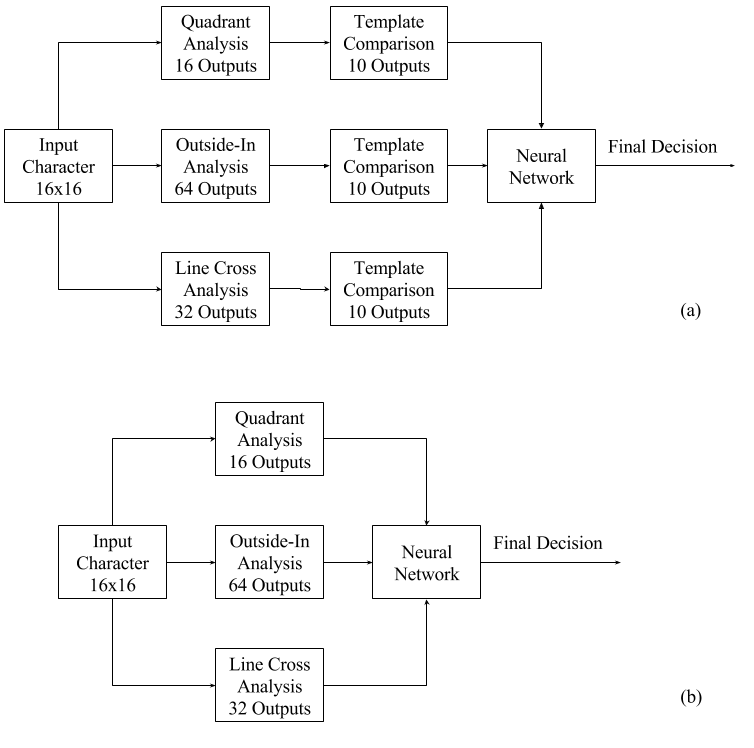
\includegraphics{fincher_approach.png}}
   \caption{(a) Structure of the Fincher’s Pre-Detection Approach, and (b) Structure of the Fincher’s Post Detection Approach}
   \label{fig:fincher_approach}
\end{figure}

%ARTIFICIAL NEURAL NETOWKR
\subsection{Artificial Neural Network}
Inspired from the nonlinear characteristics of Biological Brain System, the work performance of artificial neural networks (ANNs) can be compared to the workings of the human brain system \shortcite{ANN:2016}. While handling uncertainty and non-linearity at the same time, ANNs provide “intelligent processing functions” in order to predict, learn, and memorize \shortcite{sommer2013}. 
ANN can be applied to every situation where the input variables have a relationship with the output variables. The network for ANN consists of 3 layers in order, the input layer, hidden layer and output layer. Each layer consists of 1 or more units or neurons. 
\begin{figure}[h]
	\centering
	\captionsetup{justification=centering}
	\scalebox{.8}{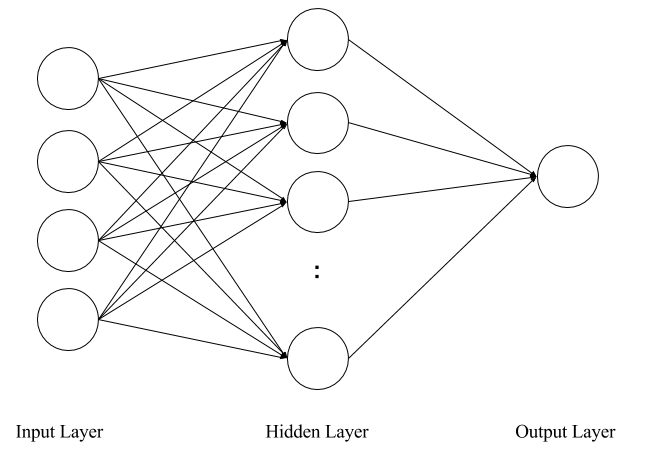
\includegraphics{Network_graph_of_a_One-Hidden_layer_ANN.png}}
	\caption{Network graph of a One-Hidden layer ANN}
	\label{fig:annexample}
\end{figure}

\figref{fig:annexample} shows a the network graph of a One-Hidden layer ANN. Each set of inputs is modified by unique weights in unit connections, and biases in unit. Training in ANN involves adjusting all the weights and biases to have the correct output. A conventional ANN uses backpropagation for its training algorithm \shortcite{Hamad2017}. Backpropagation is a training algorithm which trains the neural network from the input layer to the output layer initializing the weights and biases, and then propagate back from the output layer to the input layer to adjust the weights and biases from the differences between the generated output to the expected output. In backpropagation, each unit that receives a value gets adjusted using an activation function. This training process is repeated a number of times until training error is close to optimal, or until the network reaches the maximum number of epochs. Once backpropagation is finished, the network is trained. The weights ($w$) are adjusted by many learning algorithms such as the Error Correction Learning where the connection weigths between unit $i$ and unit $j$ are adjusted in terms of the difference between the desired and the computed value. A multilayer error correction weight adjustment formula is defined as 
\begin{equation}
w_{ij}^{new} = w_{ij}^{old} - \eta \frac{\partial  E}{\partial  w_{ij}^{old}}
\end{equation}
\noindent where $\eta$ is the learning rate - the percentage the network minimizes the error rate in each iteration and $E$ is the square of errors of the desired output and actual output which can be defined as 
\begin{equation}
E = \frac{1}{2} \sum_{j=1} \left(b_{j} - z_j\right)^2
\end{equation}
\noindent where $b$ is the desired output value, and $z$ is the actual output value.

%DEEP BELIEF NETWORK
\subsection{Deep Belief Network}
\shortciteA{koesdwiady:2016} states that the training algorithm for ANN suffer from the problem of local minima, wherein the training algorithm may get stuck in the local minima during backpropagation. Deep Belief Networks (DBN) solve this problem by adding an extra step called pre-training which is done before backpropagation that can lead to an error rate not far from optimal. Backpropagation can be used then to slowly reduce the error rate from there. Additionally, other techniques and learning algorithms cannot extract and learn features without prior knowledge of specific domains. Deep Learning could learn features with less prior knowledge. 

The training process of DBN consists of two phases, the pre-training and fine-tuning. In the pre-training process, the hidden layers of the DBN are trained greedy layer-wise. Pre-training generates the initially trained DBN with initialized weights and biases for each layer and unit. Fine-tuning further adjusts these weights and biases via backpropagation training algorithm using a labeled input data. 

DBNs are made up of stacks of Restricted Boltzmann Machines (RBM). It is a building block for multi-layer learning models of Deep Belief Networks A DBN stack RBMs to learn features to features to arrive at a high-level representation. An RBM consists of 2 layers which are the visible layer with $i$ visible units, and a hidden layer with $j$ hidden units. The RBM is an unsupervised learning algorithm that can learn useful features of the data. It takes the input and translates them into a set of numbers that represents. Then, these numbers can be translated back to reconstruct the inputs. Through several forward and backward passes, the RBM will be trained. A trained RBM can reveal which features are the most important ones when detecting patterns \shortcite{zhang:2017, Fischer2014}. The hidden units of a trained RBM represent relevant features of observations. These features can also serve as input for another RBM. The network graph of an RBM is illustrated in \ref{fig:rbmexample}.

\begin{figure}[h]
	\centering
	\captionsetup{justification=centering}
	\scalebox{.7}{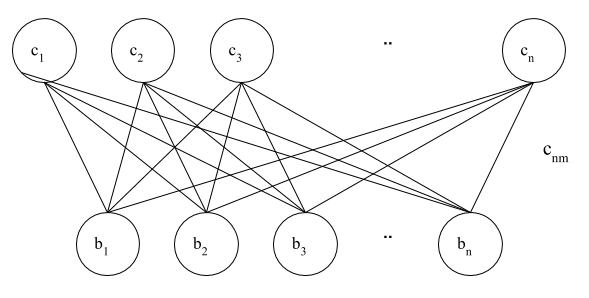
\includegraphics{Network_graph_of_RBM.png}}
	\caption{Network graph of RBM given n hidden units, and m visible units.}
	\label{fig:rbmexample}
\end{figure}

RBM defines a probability distribution, via the energy function, between each units’ weights and biases. This distribution is defined as
\begin{equation} \label{eq:1}
p(v, h) = \frac{e^{-E(v, h)}}{Z}
\end{equation}
\noindent where $Z$ is the partition function, and  $E(v, h)$ is the energy function defined as 
\begin{equation}\label{eq:2}
E(v, h) = \sum^V_{i=1} \sum^H_{j=1}  w_{ij} v_i h_j - \sum^V_{i=1}a_iv_i - \sum^H_{j=1}b_jh_j
\end{equation}
\noindent where the $v_i$ is the visible unit $i$, $h_j$ is the hidden unit $j$, $w_{ij}$ is the weight between $v_i$ and $h_j$, $a_i$ and $b_j$ are their biases. $V$ and $H$ represent the number of visible and hidden units, respectively. 
The distribution of the visible units’ weights and biases is defined as 
\begin{equation}\label{eq:3}
p(v) = \sum_H p(v, h) = \sum_H \frac{e ^ {-E(v, h)}}{Z}
\end{equation}

In RBMs, the units of the same layer are independent which do not have any connection with each other. In terms of probability, this means that the hidden variables are independent given the state of the visible variables and vice versa. Thus, the condition distributions of $p(h|v)$ and $p(v|h)$ are defined as
\begin{equation}\label{eq:4}
p(h_j = 1 | v) = \sigma\left( \sum^V_{i=1} w_{ij}v_i + b_j \right)
\end{equation}
\begin{equation}\label{eq:5}
p(v_i = 1 | h) = \sigma\left( \sum^H_{j=1} w_{ij}h_j + a_i \right)
\end{equation}
\noindent where $\sigma(x) = \frac{1}{1 + e^{-x}}$, the sigmoid function of x, the feature, element-wise.

In DBN’s pre-training, each RBM is trained individually, greedy layer-wise. The weights of each units’ connections, and each layer’s biases, are computed within this phase and saved for fine-tuning. This learning is repeated, from RBM to another, until all hidden layers are trained. This process can be expressed as follows 
\begin{equation}\label{eq:6}
p(h_j^{(l-1)} = 1 | v) = \sigma( \sum^V_{i=1} w_{ij}^{(l)}v_i^{(l)} + b_j^{(l-1)} )
\end{equation}
\noindent where $l$ corresponds to the current layer. 
The formulas and equations for RBM are based from the papers of \shortciteA{koesdwiady:2016, Fischer2014, zhang:2017}. 


\section{Weighted Average}
The Weighted Average is a signal-level fusion method that takes the weighted average of repeating information from the original inputs \shortcite{king2017, yan2011, meurant1992}. \shortciteA{king2017} claimed that using this method will ease the effect of unwanted data in the final estimation. This method can be used to estimate user activity details such as intensity, postures, and fundamental static for activity recognition systems. 

\shortciteA{yan2011} proposed the use of the weighted average method on ships traffic flow data. They used data fusion to produce a higher estimation accuracy from multiple sensors. The researchers multiplied the number of ships with its corresponding weight then obtained the average of the produced weighted inputs. They then applied a distribution method to the original data to eliminate the unwanted data. 


\section{ParseHub}
ParseHub is a free web scraping tool that collects from any JavaScript or AJAX site. This web scraping tool can also export the collected data in CSV and JSON files. The tool also has the ability to cloud host which enables the data scraped to be saved through the cloud, and schedule a run to a future time. ParseHub can scrape from hundreds of pages depending on the pricing. The Free ParseHub may only collect 200 pages worth of data in under 40 minutes. It also can run 200 pages per run. Lastly, ParseHub retains data collected for 14 days.



\section{Performance Indices}
\subsection{RMSE and MAE}
% RMSE and MAE
To evaluate a model’s performance, many studies have employed using two of the most used performance indexes: the root mean squared error (RMSE) and the mean absolute error (MAE) \shortcite{chai2014RMSEorMAE}. The RMSE is used as a standard statistical system of measurement to calculate a model's performance, especially in air quality, meteorology, and climate research studies. It is defined using this function: 

\begin {equation}
r = \sqrt[]{\frac{1}{n}\sum_{i=1}^{n}(x_i - y_i)^2}
\end{equation}

\noindent where $n$ is the number of samples, $x_i$ and $y_i$ are the errors being observed at a certain $i$. On the other hand, MAE is a measure of the absolute difference between the errors. It is defined using this function: 

\begin {equation}
r = \frac{1}{n}\sum_{i=1}^{n}|x_i - y_i|
\end{equation}

\subsection{Sensitivity Analysis}
Sensitivity analysis is a study of how much the input variables clearly affect the outcome of a model \shortcite{saltelli2000}. It is also called the simulation analysis, wherein the results are predicted based on a range of input variables. Calculating the sensitivity that is dependent on time, we calculate the sensitivity relative to the initial parameters, inputs, or conditions in the model. 

The “time-dependent” sensitivities of output $Y$ relative to every input variable are “time-dependent” derivatives is given by the equation:

\begin{comment}

\begin{equation}
\frac{\partial a}{\partial b},
\qquad
\frac{\partial a}{\partial c}
\end{equation}

\end{comment}

\begin{equation}
\abs*{\frac{\partial Y}{\partial X_i}}_{X^0}
\end{equation}

\noindent where, $Y$ is the output and $X_i$ is the input factor. $X^0$ indicates that the derivative is taken at some fixed point in the space of the input. This shows that per input of the model, the ratio of its derivative with respect to its output is computed to get the sensitivity.

\begin{comment}
\noindent where, the $\partial a$ is the output and the $\partial b$ and $\partial c$ are the inputs of neural networks. This shows that per input of the model, the ratio of its derivative with respect to its output is computed to get the sensitivity.
\end{comment}

Several researchers have been applying sensitivity analysis to their models, particularly to the models which uses neural networks. In \shortciteA{hunter2000}, they applied sensitivity analysis of neural network inputs to their trauma survival prediction model to analyze the Trauma and Injury Severity Score (TRISS) variables used in their model. Their experiments on the variable’s sensitivity show that age is the most prominent variable in predicting survival. The researchers defined three approaches to sensitivity analysis. First is to introduce noise to every input variable and to observe its effects to the results. Second is to examine the derivatives of the weights of the input variables. Last is the proposed form of analysis based from the missing value problem approach. 

In \shortciteA{refenes1994}, they performed sensitivity analysis to evaluate their model on stock performance using neural networks. They used scatter plots to visually analyze the change in their network output (the likelihood of a sample being a target) with respect to the network input (stock factors). Based on their result, they were able to explain the predictive behavior of their neural network output by using sensitivity analysis. Furthermore, they were able to conclude that compared to regression models, their model can model the situation more convincingly.

               %-- includes LaTeX source file for Chapter 3: Theoretical Framework
                                  %-- your job: **EDIT THIS FILE** to indicate your theoretical framework
                                  
                                  \chapter{Research Design}
\label{resdes}
\begin{comment}

\end{comment}

\begin{figure}[h]
	\centering
	\captionsetup{justification=centering}
    \scalebox{.40}{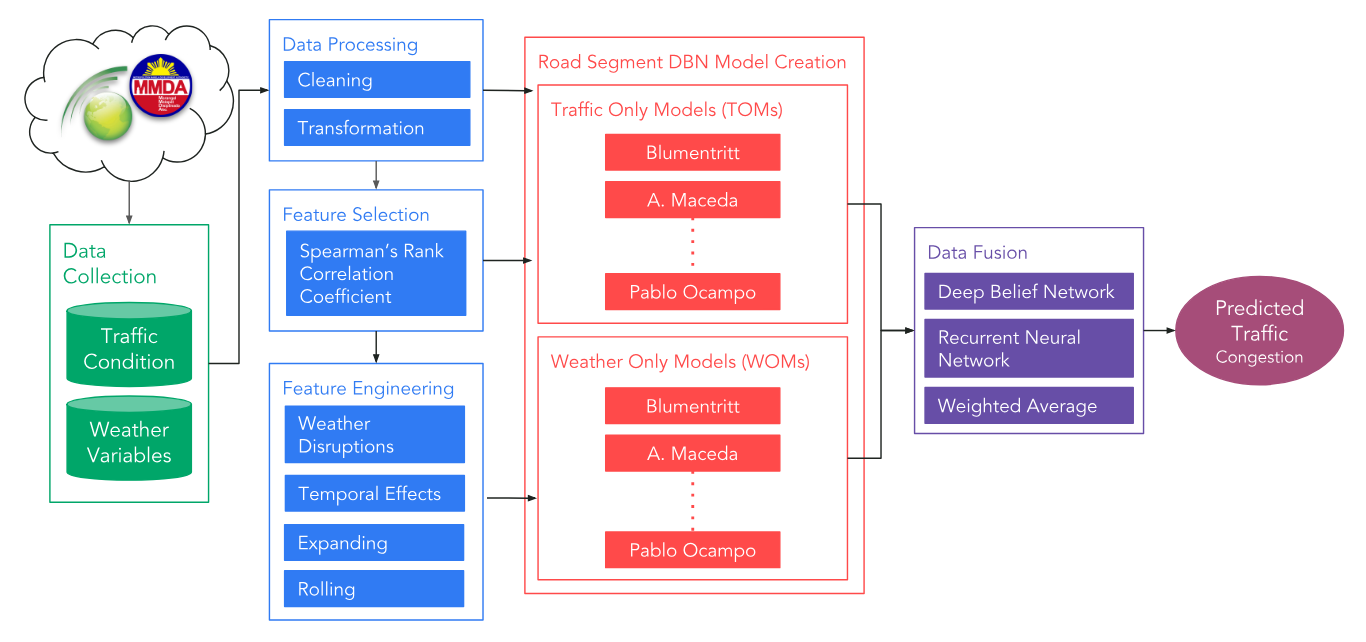
\includegraphics{THESIS_ResearchDesignFinal.png}}
	\caption{Research Framework}
	\label{fig:framework}
\end{figure}




Figure \ref{fig:framework} illustrates the whole framework for the research. First, this research collected historical traffic condition from MMDA and historical weather variables from WWO. These raw data were cleaned and re-sampled to match the time intervals of the data using linear interpolation and was transformed to their normalized values. The data was explored and analyzed to identify seasonality and trends present for both traffic and weather. Analysis and insights collected was used to select and engineer features to use in the model to predict traffic. These features include rolling and expanding window features, in-depth statistical features of traffic such as the mean of past traffic of a certain time period. 

The final variables and engineered features were fed into the Traffic-Only Models (TOM) and Weather-Only Models (WOM), which were developed in DBN, for the 14 road segments in Manila for both wet and dry season. Additionally, analyses were evaluated through the training of the models. Different fusion techniques were explored and evaluated. Specifically, fusing at the feature and decision level were evaluated. Then, different fusion techniques (i.e. DBN, RNN, and WA) for fusing at the decision level were explored. The model was evaluated using RMSE and MAE. The model’s sensitivity was also explored to analyze the relevance of input variables. Sensitivity analysis is also performed to achieve higher accuracy through calibration of hyper parameters. 

\section{Data Collection}
 \label{rd_datacollection}
There were two datasets collected: traffic and weather. The traffic dataset was obtained from Metro Manila Development Authority (MMDA) traffic monitoring system. The weather dataset was collected from World Weather Online (WWO). Both datasets were collected from January 2015 to December 2015.

\subsection{Traffic Dataset}
There were two limitations found from the traffic dataset. First is that the traffic conditions were only represented as \textit{light} (L), \textit{moderately light} (ML), \textit{moderate} (M), \textit{moderately heavy} (MH), and \textit{heavy} (H). Since this dataset only had five values to classify the traffic condition in a particular road segment, this might cause underfitting in our model since it was used as input for a regression problem. Moreover, it could also contribute to poor correlation as these five values were correlated with continuous weather variable values. To have the traffic conditions be continuous values, they were converted to their equivalent estimated traffic speed provided by the MMDA (see Table \ref{table_traffic_condition}). These speeds are further converted to congestion levels, represented as their reciprocal so that the data would be easier to interpret such that higher value means higher congestion level.

\begin{table}[h]
\centering
\caption{Traffic speed equivalent of traffic conditions}
\label{table_traffic_condition}
\begin{tabular}{|l|r|}
\hline
\textbf{Traffic Condition} & \multicolumn{1}{l|}{\textbf{Equivalent Speed (kph)}} \\ \hline
Light (L)                  & 36 - 60                                             \\ \hline
Moderately Light (ML)                  & 31 - 35                                            \\ \hline
Moderate (M)               & 16 - 30                                             \\ \hline
Moderately Heavy (MH)                  & 11 - 15                                             \\ \hline
Heavy (H)                  & 0 - 10                                              \\ \hline
\end{tabular}
\end{table}

Another limitation was that the traffic dataset contains missing records. Out of 935,200 records, there were 93 rows wherein the traffic condition of that road segment in that particular time interval was not recorded as indicated by \textit{none} (N) condition. Furthermore, having only 935,200 records from a sample from 2015, having a 15-minute interval for 14 road segments, meant that 45,920 records were missing as well. This implied that inconsistencies may occur as the missing data would need to be filled to make the data continuous. To do this, those missing values were replaced through linear interpolation.

Apart from the limitations, there were other factors considered in this study. Since this study is only concerned road segments from Manila, only the road segments under it were used. As a result, 14 out of 142 road segments were only considered: 7 from Roxas Boulevard and 7 from España.

\subsection{Weather Data}
The collected weather dataset from WWO featured a complete hourly reading of the weather variables for Manila. One downside of this dataset, however, was that the weather data generalizes the weather for the whole city. This implied inconsistencies when correlating the traffic condition to the weather variables as the weather at one road is not the same as the weather of another, despite being in the same city.

Additionally, the hourly weather dataset needed to be matched with the 15-minute interval of the traffic dataset. This was done by resampling and linear interpolating the dataset to have a 15-minute time interval.

\section{Exploratory Data Analysis}
To be able to extract the relationship between these two independent datasets, we need to understand the underlying pattern of each other and its effect on one another. In this study, we approached this in three steps. First, patterns of traffic and weather are explored as independent entities. This patterns include seasonality and trends of each variable, and disruptions present for each variable. From this, patterns are compared to identify the relationship between the two entities. Once these patterns are bridged, instances of weather disruption to traffic are derived by associating the weather variables that may be a contributing factor to traffic.

\subsection{Seasonality Analysis}
Seasonality refers to a predictable pattern of a time series data that regularly repeats after a number of intervals. To identify the short-term seasonality of weather variables, we analyzed the similarity between an observation and time lags between them through autocorrelation. Lags refer to the delay of one observation on another. For instance, the delay between the temperature observations at June 18 and June 19 is indicated by a one-day lag.

\subsubsection{Weather Seasonality}
%Seasonality
Assessing the seasonality of weather variables is useful in our study as it allows us to identify the span of the trend of a specific weather variable. Observably, one weather variables that do have a daily pattern is temperature. Its pattern starts by rising in the morning, peaking in the afternoon, then starts falling in the evening. There are also weather variables, on the other hand, that does not have an observable pattern. One example of this is precipitation. Unlike temperature that has an observable pattern per day, the occurrence of precipitation is situational. 

%Trend
Once we are able to identify the short-term seasonality of individual weather variables, we zoom in further in given observations, based on the identified seasonality time spans, and analyze how similar are these in terms of trend. For instance, we will analyze how similar are temperature on one observation and its previous day, and how different are precipitation on one observation and its previous day.

\subsubsection{Weather Disruptions}
Assessing the effect of a disruption of one weather variable to another weather variable was also explored. After analyzing the seasonality of weather, its trend that can be defined as normal is defined. Any other patterns that are significantly different from the defined normal trend of any weather variable is explored, and compared with other aligned weather variables. 

\subsubsection{Traffic Seasonality}
On an average day, traffic could be linked with the people's daily transportation demand. One example of these is the daily commute of people, attributed to their organizational duties (i.e. 9 to 5 jobs) and academical duties. Built upon these expected demands, the daily seasonality of traffic has been established, following the concept of peak hour. Peak hour refers to the busiest hour where traffic is expected to rapidly rise. In the case of Metro Manila, peak hours are expected to occur from 7 AM to 10 AM, when people leave their home to go to their respective organizations, and 4 PM to 7 PM, when they depart their organizations and return home \cite{metro_manila_peak_hour}.

However, knowing that there are other contributing factors to traffic, its pattern is inconsistent despite its people’s daily commute schedule remains constant as the years go by. Given this problem, it is significant to identify the more accurate estimate of the seasonality of traffic, considering that these contributing factors are already embedded in the day-to-day traffic. These could be done by analyzing a road segment, as an individual point-to-point segment, and analyzing a road segment, as a part of the whole road, taking into account its connected roads. 

\subsubsection{Traffic Disruptions}
As traffic seasonality was explored, traffic patterns that do not follow the defined pattern is explored. Disruptions in the patterns of traffic is compared with the explored disruption in weather to derive an analysis whether the disruptions of traffic and weather are connected. 

\section{Correlation Analysis}
The relationship of weather and traffic is then explored through correlation analysis. In this analysis, correlation between weather factors, connected roads, and engineered traffic features with traffic is explored in order to have a better understanding of the effect of weather to traffic, especially in time periods where weather is most expected to disrupt traffic such as periods typhoons are present. Relationships derived from the correlation was verified through comparative analysis between the defined weather and traffic patterns

First, the relationship of each weather variable to each other was explored in order to extract which weather variables are significant with respect to traffic condition. Significant weather variables that are both highly correlation with another variable, but less correlated with traffic than the other variable is removed to reduce redundancy. Then, the relationship between connected roads was explored. In this analysis, the intensity of one road segment and its effect to the connected road segment was analyzed through correlation. The correlation growth from the first road segment, to the nth connected road segment was also analyzed.  Lastly, the relationship between the engineered traffic features to the current traffic feature. Before exploring this relationship, traffic features were engineered from the current traffic feature in order to give information of the immediate past traffic, and its relationship with the current traffic. These engineered traffic features include rolling and expanding window features, statistical description of past time period such as the mean traffic two (2) weeks ago, and flags for significant traffic patterns such as the work day and peak hours. Exploring the relationship between this engineered traffic features with the current traffic feature also give a better representation of the effect of disruptions present in the immediate past to the current traffic. 

As mentioned, rolling and expanding window features were engineered to represent the immediate past traffic. Rolling and expanding traffic features were generated for window sizes \textit{4, 8,  24, 48}, and \textit{96}, with each window representing a 15-minute time interval. Thereby, the generated window sizes translates to \textit{1, 2, 6, 12}, and \textit{24}-hours time interval. The statistical features such as the mean, minimum and maximum for both rolling and expanding windows were generated to describe the immediate past traffic conditions given a specific window size. 



%TRAFFIC MODEL CREATION
\section{Model Implementation}
Features were engineered in order to represent the immediate past traffic, and other trends and patterns of traffic. Additionally, weather features were selected through correlation analysis. These features are as follows:

\begin{enumerate}
\item Temporal Information of the respective traffic record represented as Month, Day, Hour, Minute, Day of Week,
\item Traffic a Day before represented as L, ML, M, MH, H
\item Traffic 6 weeks ago represented as L, ML, M, MH, H
\item Current Traffic represented as L, ML, M, MH, H
\item Rolling and Expanding Traffic Features (mean, max, and minimum) for windows 4, 8, 24, 48, and 96 represented as L, ML, M, MH, H,
\item Weather Variables (wind speed, wind gust, temperature, humidity, dew point, precipitation, visibility, pressure, cloud cover, heat index, and feels-like) represented in their respective measurements 
\end{enumerate}

A model implemented using Deep Belief Network (DBN) used these features that represent the past traffic to predict the current traffic condition intensity. 

\subsection{Prediction Models}
According to the framework in \ref{fig:framework}, two models were implemented using Deep Belief Network (DBN): the Traffic-Only Model (TOM) and the Weather-Only Model (WOM). TOM considers historical traffic condition intensity to predict traffic, while WOM only considers historical weather variables to predict traffic. In this study, DBN models were implemented with the open source machine learning framework in python, \textit{tensorflow}. The architecture of the model for TOM and WOM are different, and suits the dataset used. For TOM, there are two hidden layers with 14, and 390 units respectively. TOM was trained with 15 epochs during the pre-training phase, and 150 epochs during the fine-tuning phase. For the WOM, there are 3 hidden layers with 7, 70, and 100 units respectively. WOM was trained with 11 epochs during the pre-training phase, and 150 epochs. The learning rate for both DBN and RBM for both models is 0.01. The activation function for both models is the $relu$ function. 

Deep Belief Networks (DBN) are  made up of stacks of Restricted Boltzmann Machines. The training for DBN consists of two phases: pre-training and fine-tuning. In pre-training, each RBM is trained individually, and weights and biases of layers are fixed. In fine-tuning, the weights and biases of the whole network are updated via back propagation using labeled input data. 

Figure \ref{fig:dbntraining} shows the process of how TOM and WOM using DBN was trained for prediction. The training process consists of three phases. In the first phase, the stacks of RBM (sRBM) within the network is  trained individually. At the end of this phase, the weights and biases of the whole DBN are initialized. In the second phase, the DBN fine tunes the initialized weights and biases using backpropagation algorithm. The network after stage 2 is the trained and enhanced DBN. In the third phase, the network predicts the future traffic condition using a testing dataset.

\begin{figure}[h]
	\centering
	\captionsetup{justification=centering}
	\scalebox{.8}{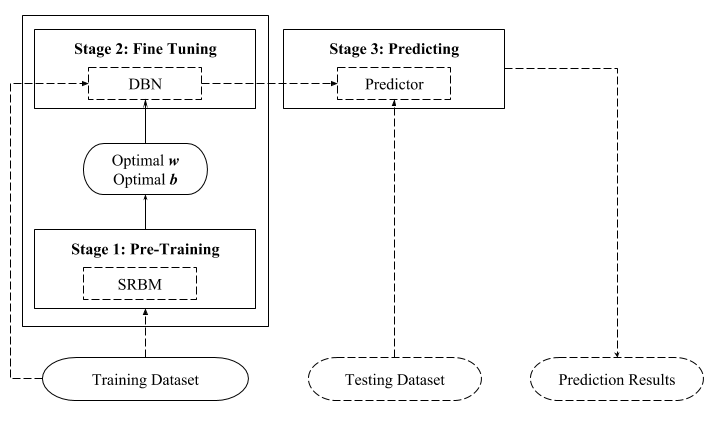
\includegraphics{dbntraining.png}}
	\caption{Structure of DBN Training Process}
	\label{fig:dbntraining}
\end{figure}

For the pre-training phase, the sRBM performs a number of forward and backward passes until the reconstructed data is close to the original input. The process of backward and forward passes is performed using the equations \ref{eq:4} and \ref{eq:5} to compute for the conditional probability of the hidden unit $h_j$ and visible unit $v_i$, respectively. 

%Fine Tuning
For the fine-tuning phase, the loss function and activation function is defined.
The loss function for the softmax layer to improve the learning rate uses the cross-entropy equation between the visible and hidden units. The cross-entropy function is defined as 
\begin{equation}
C = -\frac{1}{n}\sum_x [y ln a + (1 - y) ln (1-a)]
\end{equation}
\noindent where $n$ is the size of the training data, $x$ is the training input, $y$ is the desired output, and $a$ is the unit’s output. 
For the activation function in the fine-tuning phase, the rectifier function was used for its nonlinearity activation capability. The rectifier function is defined as 
\begin{equation}
f(x) = x^+ = max(0, x)
\end{equation}


\subsection{Data Fusion Model}
This study’s framework will evaluate two fusion approaches: Feature In-Decision Out (FEI-DEO) and Decision In-Decision-Out (DEI-DEO). In the first approach, traffic and weather features are fused in one dataset first before being used to predict traffic. While the latter approach predicts traffic through TOM and WOM, and fuses the prediction of both models into one final prediction. DBN is used in the FEI-DEO approach, while three algorithms are used in the DEI-DEO approach which are Weighted Average (WA), Recurrent Neural Network (RNN) and DBN. 


%WEIGHTED AVERAGE
\subsubsection{Weighted Average} 
The weighted average data fusion method used the predicted traffic from TOM and WOM. Both predictions was multiplied with its corresponding weight. Each weight was assigned based on the importance of the variable considered while keeping in mind the sum of the weights should be equal to 1. Then, the mean of the weighted predictions of both TOM and WOM will be calculated. The result will be the fused final traffic prediction.


%NEURAL NETWORK
\subsubsection{Neural Network}
The fusion model was also developed in two neural networks: Recurrent Neural Network (RNN) and Deep Belief Network (DBN) in evaluating DEI-DEO fusion approach. Only DBN was implemented in evaluating FEI-DEO approach.

In FEI-DEO, the traffic congestion intensity and weather variables were fused into one dataset before feeding it into the prediction model. The network will be trained to predict the traffic condition based from both traffic and weather in one model for the current time period $t$. The training of the network will continuously adjust weights and biases from comparing the generated output with the actual traffic condition. 

The DBN for FEI-DEO fusion have 1 input layer, 3 hidden layers, and 1 output layer. There are 5 epochs for the pre-training phase, and 150 epochs for the fine-tuning phase. The learning rate for both DBN and RBM is 0.01. 

In DEI-DEO, the traffic congestion intensity was predicted first with two prediction models, TOM and WOM. The prediction by these two prediction models was used into another model that will fuse the two predictions into one improved final prediction. The network will be trained to predict the traffic congestion intensity for the current time period $t$ through backpropagation by comparing the generated traffic condition prediction to the expected prediction, and adjusting the weights and biases of units and layers to fuse the two decisions to arrive to a prediction close to the expected. The input layer will have the predicted traffic condition of TOM and WOM. 

The RNN for DEI-DEO fusion have only have 1 input layer, 1 hidden layer, and 1 output layer. The number of units for the hidden layer of the RNN will be determined through trial and testing starting from 5 to 100 units. 

The DBN for DEI-DEO fusion will only have 1 input layer, 3 hidden layers, and 1 output layer. The DBN for the DEI-DEO fusion will be similar with the TOM and WOM in terms of it’s hidden layer structure, and epochs. However, instead of historical traffic and weather data as its input, predictions made by TOM and WOM is used and fused into one final prediction. 

%TRAINING
\section{Training}
The collected dataset for traffic and weather was divided into two subsets; wet and dry season. The wet season dataset consists of data from the months of May to October 2015, while the dry season dataset consists of data from the months of November to April 2015. The models was tested on these datasets to evaluate the inclusion of weather variables. 

Datasets was split into training and testing datasets. The Training dataset was used during the pre-training and fine-tuning of the model. In the fine-tuning phase of the training of the model, the training dataset was labeled with the expected output so as to verify and adjust the weights and biases back from the pre-training. The labels consists of the expected traffic condition given the input data. All data fed into the network are already be normalized. 

The training dataset for both prediction models Traffic Only Model and Weather Only Model consists of data from the months of May to August was used for evaluating wet season, and months of January to April was used for evaluating dry season. In turn, the testing dataset made use of the remaining months of the season: September to October for the wet season, and November to December for the dry season.  

%[Training Data of TOM]
The training dataset for the Traffic-Only Model consists of the following information in a 15-minute time interval: 
Temporal Information of the respective time period (i.e. month, hour, minute, day, and day of week),
Traffic condition intensity a day before the respective traffic,
Flags on working day and peak hour of the respective time period ,
Rolling and expanding window features (which consist of the minimum, maximum, and mean for each window) for the immediate past traffic of the respective traffic,
Mean of the traffic 2 weeks before the respective traffic;
In further experiments, the inclusion of the information regarding working days, peak hours, and immediate past traffic was compared and evaluated. The label for the training dataset consists of actal the 15-minute time interval of the traffic condition intensity of the respective time of the bound of the road segment to be predicted. For visualization purposes, the input including the labels is illustrated in Figure \ref{fig:TOM_TrainingTestingInput}


\begin{figure}
  \centering
  \captionsetup{justification=centering}
 \scalebox{.70}{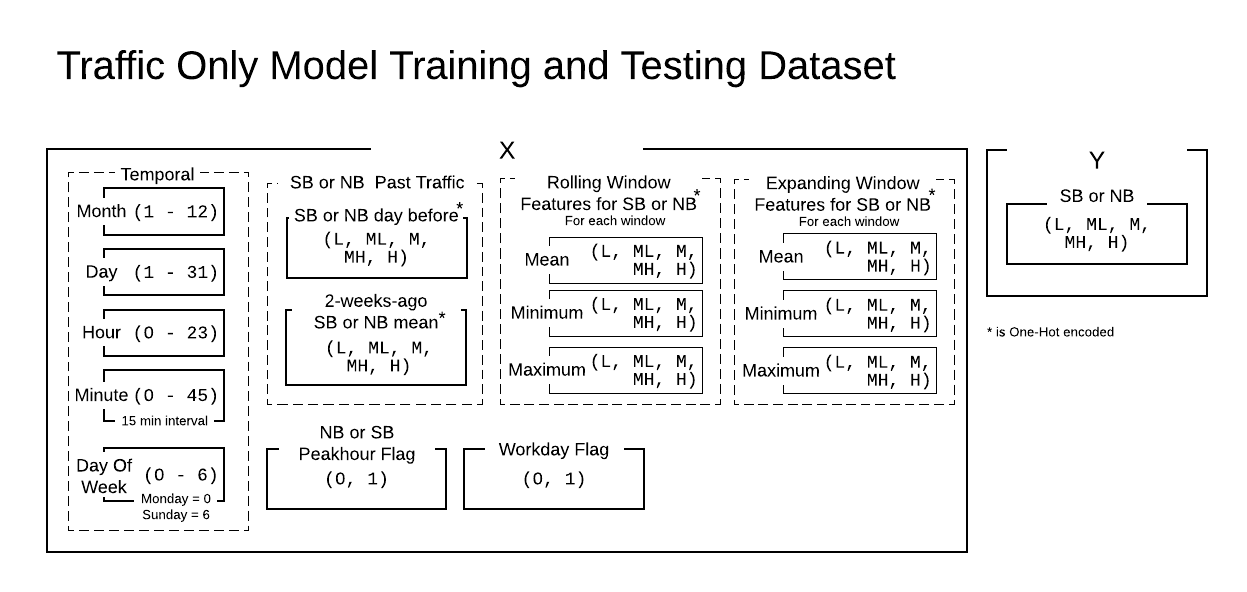
\includegraphics{TOM_TrainingTestingInput.png}}
  \caption{A summary on the contents of the Traffic Only Model Training and Testing Dataset}
  \label{fig:TOM_TrainingTestingInput}
\end{figure}


%[Training Data of WOM]
The training dataset for the Weather-Only Model consists of the following information in a 15-minute time interval: 
Temporal Information of the respective time period (i.e. month, hour, minute, day, and day of week), and;
Current weather variables (e.g. temperature, precipitation, wind speed, etc.) of the respective time period
In further experiments, different combinations of weather variables is compared and evaluated. The label for the training dataset consists of the actual 15-minute time interval of the traffic condition intensity of the respective time of the bound of the road segment to be predicted. 

%[Training Data of DF Fusion Model]
For the feature-level fusion model, the training dataset consists of merged training dataset used in the Traffic-Only and Weather-Only Models. The months for the training and testing datasets for this fusion model is the same as Traffic-Only and Weather-Only Model. 

For the decision-level fusion model, the training dataset consists of the predicted traffic for the month of September and November generated by the Traffic-Only and Weather-Only model. The testing dataset consists of the predicted traffic for the month of October and December. The label for the training dataset will consist of the 15-minute time interval of the actual traffic condition intensity of the respective time of the bound of the road segment to be predicted. 


\section{Evaluation}
%[Comparing of Performances]
The performance of the all models and algorithms (DBN, RNN, and WA) was evaluated using RMSE and MAPE. The performance of the fusion model fusing in the feature level (FEI-DEO) and in the decision level (DEI-DEO) was first evaluated. In evaluating DEI-DEO, the performance of TOM and WOM models were first evaluated before the fusion model/s. To evaluate the performance of TOM and WOM, different feature combinations are were. The performance of the model with these different feature combinations are compared with each other to see which input variables are needed in predicting the traffic condition intensity in current time period $t$. Then, three fusion techniques, namely weighted average, RNN and DBN, were compared and evaluated to see the accuracy of the final prediction. Additionally, the performance of the TOM and the final prediction of the DEI-DEO fusion model was evaluated to see relevance of the inclusion of weather variables as a factor in predicting traffic. 

The model’s sensitivity was also explored to analyze the relevance of input variables. Sensitivity analysis is also performed to achieve higher accuracy through calibration of hyper parameters. Specifically, the sensitivity for the models TOM, WOM and DEI-DEO fusion center in DBN will be evaluated. In evaluating the sensitivity for TOM and WOM, different combinations of input variables will be evaluated to see how much the inclusion and removal of a variable affects the final prediction. The parameters of the network was also experimented with, specifically the number of hidden layers and its units, the number of epochs for pre-training and fine-tuning and the batch size was tinkered. 


               %-- includes LaTeX source file for Chapter 3: Research Design
                                  
                                   \chapter{Results and Discussion}

This chapter discusses the exploratory data analysis of the collected traffic and weather data to identify seasonalities, disruptions, and correlations. It also discusses the experiments performed in building the prediction model, as well as its evaluation.

\section{Pattern Analysis}
\subsection{Traffic Analysis}

Analyzing the autocorrelation of traffic (see Figure \ref{figure_autocorr_week}), it could be observed that in spite of its daily pattern, its succeeding days are loosely correlated with the present one. Interestingly, though, the traffic pattern of the previous day is similar as much as the succeeding days or even the week after. Furthermore, compared with its previous days, it could be observed the present traffic is more correlated with its 7-days-ago pattern or its previous week (e.g. present Monday with last week's Monday).


\begin{figure}
  \centering
  \captionsetup{justification=centering}
  \scalebox{.65}{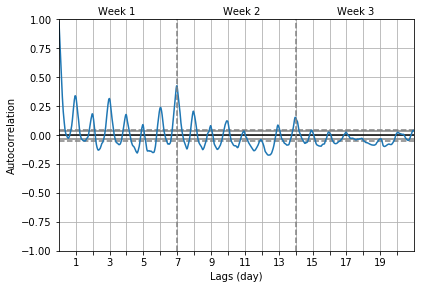
\includegraphics{figure_autocorr_week.PNG}}
  \caption{Autocorrelation of traffic revealing its daily and weekly seasonality}
  \label{figure_autocorr_week}
\end{figure}


\label{figure_autocorr_week}

Viewing its pattern in a longer term (i.e. month-long, year-long), nevertheless, its weekly pattern becomes looser as months go by (see Figure \ref{figure_autocorr_traffic_month}). In other words, it is recommended to expect a certain pattern to last for only four weeks at most. Further examining its seasonality, it could also be observed that it does not have a yearly seasonality, and its seasonality fades out as time passes by. In simple terms, the traffic pattern in January 2015 is not the same with January 2016. Rather, the traffic pattern in December 2015 is closer to the pattern of January 2016.


\begin{figure}[h]
  \centering
  \captionsetup{justification=centering}
  \scalebox{.65}{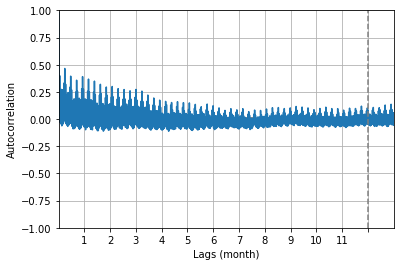
\includegraphics{figure_autocorr_traffic_month.PNG}}
  \caption{Autocorrelation of traffic showing no monthly nor yearly seasonality}
  \label{figure_autocorr_traffic_month}
\end{figure}



\subsubsection{Previous Day}

Comparing the average traffic between working days and non-working days in one month, we could see a significant difference in terms of intensity and pattern (see Figure \ref{figure_workingday_comparison}). Majority of intense traffic occurs at working days. Table \ref{table_traffic_cond_workingday} shows that heavy traffic consists 10.584\% of the working day dataset, while only 0.301\% of the non-working day dataset. Moreover, light traffic consists of only 51.819\% of the working day dataset while it accounts for 76.973\% of the non-working day dataset.

This, in terms of trends, indicates that working day traffic may follow the peak hour-driven traffic pattern. Comparing the trend between working day and non-working day, there can be an observable trend during working days due to the high variance in terms of intensity. In Figure \ref{figure_workingday_comparison}, it could be observed that the trend of traffic goes up at around 6:00. From that, it settles as it approaches around 11:00. Then, northbound and southbound follows their own trend. For northbound, the traffic settles over the afternoon and begins to rise at around 18:00 then drops at around 20:00. Meanwhile, for southbound, the traffic settles during the afternoon and drops similarly at around 20:00. Given these differences in terms of trend, in defining a specific peak hour, we must consider non-working days as an inconsistent case if compared with working days.


\begin{figure}[h]
  \centering
  \captionsetup{justification=centering}
  \scalebox{.65}{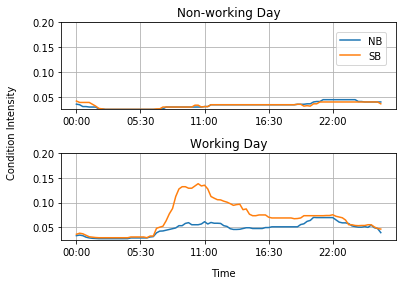
\includegraphics{figure_workingday_comparison.PNG}}
  \caption{Comparison of the average traffic in one month between working and non-working revealing the lack of intense traffic for non-working days}
  \label{figure_workingday_comparison}
\end{figure}




\begin{table}[h]
\centering
\caption{Comparison of traffic condition distribution between working and non-working}
\label{table_traffic_cond_workingday}
\begin{tabular}{|l|r|r|}
\hline
\textbf{Traffic Condition} & \textbf{Working Day} & \textbf{Non-working Day} \\ \hline
L                          & 51.876\%             & 76.973\%                 \\ \hline
ML                         & 4.051\%              & 3.085\%                  \\ \hline
M                          & 31.917\%             & 19.461\%                 \\ \hline
MH                         & 1.573\%              & 0.180\%                  \\ \hline
H                          & 10.584\%             & 0.301\%                  \\ \hline
\end{tabular}
\end{table}






\subsubsection{Previous Week}
In Figure \ref{figure_traffic_day_vs_week}, it could be observed how closer the traffic pattern is with its one-week-ago pattern compared with its two-days-ago pattern. Referring at the identified traffic seasonality in Figure \ref{figure_autocorr_week}, we could see how an observation in traffic appears to be more seasonal with its previous weeks as compared with the preceding days, with exception to the previous day.


Comparison between traffic’s two-day-ago pattern and one-week-ago pattern showing that previous week traffic is more similar despite its difference in terms of days

\begin{figure}[h]
  \centering
  \captionsetup{justification=centering}
  \scalebox{.65}{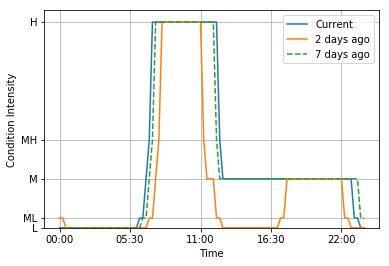
\includegraphics{figure_traffic_day_vs_week.PNG}}
  \caption{Comparison between traffic’s two-day-ago pattern and one-week-ago pattern showing that previous week traffic is more similar despite its difference in terms of days}
  \label{figure_traffic_day_vs_week}
\end{figure}



\subsection{Weather Analysis}

Performing Spearman's rank correlation on weather variables against traffic, in general, reveals that they have a weak correlation (see Figure \ref{figure_corr_trafficweather}). One possible reason for this is the effects of weather to traffic is not immediate. For instance, changes in traffic pattern are not immediately seen upon the start of precipitation. Instead, it can be seen after a while as precipitation continues building up. To address this problem, an exploratory analysis between each weather variables and traffic are conducted, exploring their commonalities in terms of seasonality and trends.


\begin{figure}[h]
  \centering
  \captionsetup{justification=centering}
  \scalebox{1}{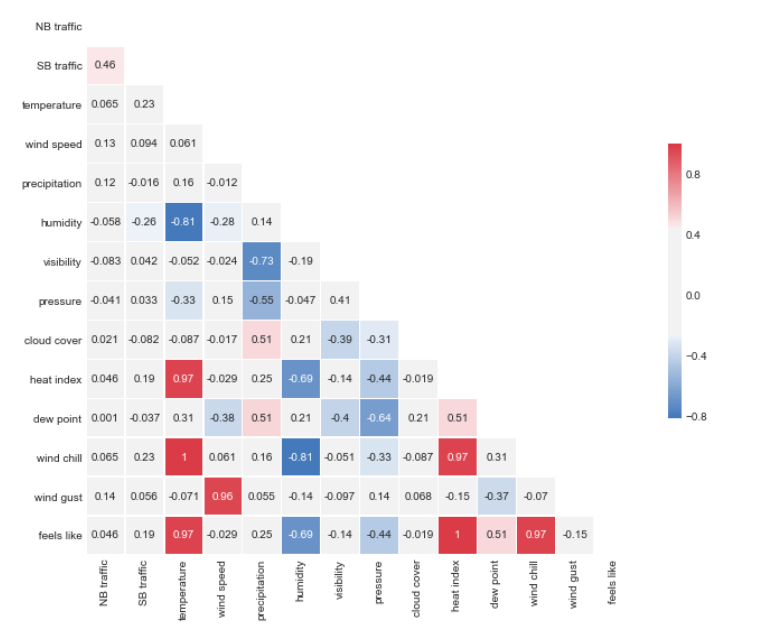
\includegraphics{figure_corr_trafficweather.PNG}}
  \caption{Correlation heatmap of traffic and weather variables showing a weak correlation between them}
\label{figure_corr_trafficweather}
\end{figure}



\subsubsection{Seasonality}

Similar to traffic, the autocorrelation of each weather variable reveals that all of them have a daily seasonality (see Figure \ref{figure_autocorr_weather}). Notably, the majority of them are able to maintain their seasonality for days or even a week. Nevertheless, these are not true for weather variables such as precipitation, visibility, wind speed, and wind gust, which are seasonal to their previous day yet have a weak relationship with it.


\begin{figure}[h]
  \centering
  \captionsetup{justification=centering}
  \scalebox{1}{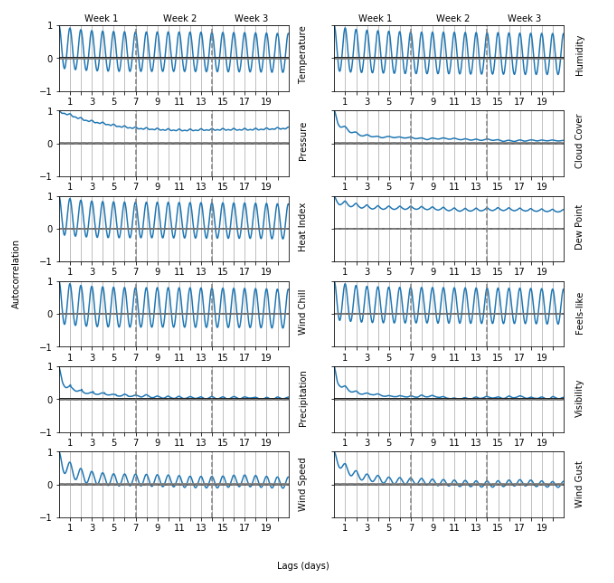
\includegraphics{figure_autocorr_weather.PNG}}
  \caption{Autocorrelation of weather variables showing the presence of daily seasonality}
\label{figure_autocorr_weather}
\end{figure}

%Autocorrelation of weather variables showing the presence of daily seasonality
%\label{figure_autocorr_weather}

\subsubsection{Trend}

As traffic is able to maintain a relatively moderate seasonality with its previous days, weather variables whose seasonalities are characterized similarly will be explored. These will include temperature, pressure, heat index, wind chill, humidity, dew point, and feels-like. To define their normal trend, their daily average per time intervals will be utilized, given by its daily seasonality. In consideration for the case of traffic, however, priority will be given to the SB traffic as it has a relatively stronger relationship with other weather variables as compared with NB traffic, and only working days on a given month will be considered with respect to its previous day seasonality.

\paragraph{Temperature, Heat Index, Feels-Like and Wind Chill}

Figure \ref{figure_traffic_vs_tempheatfeelswind} illustrates a one-month visualization of the normal trend of temperature, heat index, feels-like and wind chill against traffic. From the initial correlation analysis mentioned earlier (see Figure \ref{figure_corr_trafficweather}), temperature, heat index, feels-like and wind chill has a weak correlation of 0.230, 0.190, 0.230 and 0.190 respectively with traffic. A reason for this is despite that they match in terms of their morning trend, their evening trend significantly differs. Moreover, interpreting this relationship, it only shows the transition of dawn to morning, or simply the beginning of the morning peak hour.


\begin{figure}[h]
  \centering
  \captionsetup{justification=centering}
  \scalebox{.65}{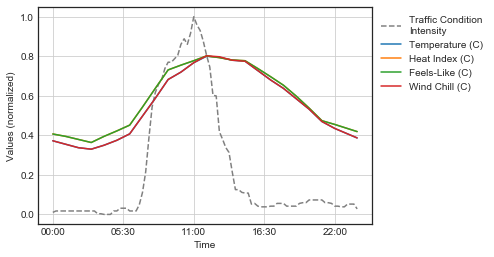
\includegraphics{figure_traffic_vs_tempheatfeelswind.PNG}}
  \caption{Comparison of the normal pattern of temperature, heat index, feels-like and wind chill with the normal pattern of traffic}
\label{figure_traffic_vs_tempheatfeelswind}
\end{figure}


%Comparison of the normal pattern of temperature, heat index, feels-like and wind chill with the normal pattern of traffic
%\label{figure_traffic_vs_tempheatfeelswind}

\paragraph{Pressure}

Figure \ref{figure_traffic_vs_pressure} shows a one-month visualization of the normal trend of pressure and traffic. At initial glance, it resembles the traffic pattern in a subtle way. However, looking at the initial correlation analysis earlier (see Figure \ref{figure_corr_trafficweather}), pressure appeared to have a significantly weak correlation with traffic, at 0.033. One notable difference between pressure and traffic is that pressure rises again during the evening up to dawn, following its relationship with temperature \shortcite{aguado2007understanding}.


\begin{figure}[h]
  \centering
  \captionsetup{justification=centering}
  \scalebox{.65}{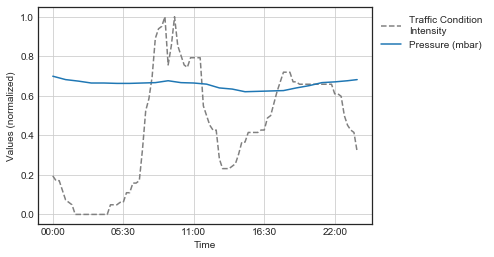
\includegraphics{figure_traffic_vs_pressure.PNG}}
  \caption{Comparison of the normal pattern of pressure with the normal pattern of traffic}
\label{figure_traffic_vs_pressure}
\end{figure}

%Comparison of the normal pattern of pressure with the normal pattern of traffic
%\label{figure_traffic_vs_pressure}

\paragraph{Humidity}

Figure \ref{figure_traffic_vs_humidity} illustrates a one-month visualization of the normal trend of humidity and traffic. Basing on the initial correlation (see Figure \ref{figure_corr_trafficweather}), humidity has a weak correlation of -0.260 with traffic. Comparatively, this could be interpreted in the same way as temperature yet reversed due to its negative relationship, following the relationship of temperature and humidity \shortcite{paull1999effect}. This is further supported by the strong negative relationship between temperature and humidity with a value of -0.810.


\begin{figure}[h]
  \centering
  \captionsetup{justification=centering}
  \scalebox{.65}{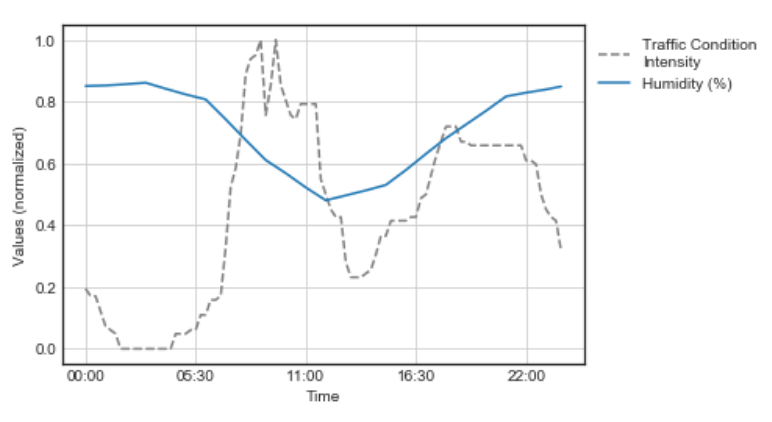
\includegraphics{figures/figure_traffic_vs_humidity.PNG}}
  \caption{Comparison of the normal pattern of humidity with the normal pattern of traffic}
\label{figure_traffic_vs_humidity}
\end{figure}

% Comparison of the normal pattern of humidity with the normal pattern of traffic
% \label{figure_traffic_vs_humidity}

\paragraph{Dew Point}

Figure \ref{figure_traffic_vs_dewpoint} shows a one-month visualization of the normal trend of dew point and traffic. Upon initial inspection, there is a subtle similarity between its pattern with the pattern of traffic. However, referring to the initial correlation (see Figure \ref{figure_corr_trafficweather}), dew point has a significantly weak correlation of -0.037 with traffic. Rather, this similarity in terms of form may be due to its relationship with pressure \shortcite{gaul1952relation}.

\begin{figure}[h]
  \centering
  \captionsetup{justification=centering}
  \scalebox{.65}{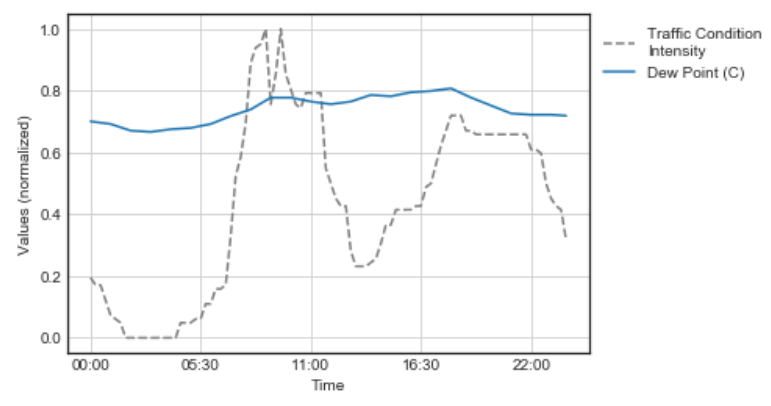
\includegraphics{figures/figure_traffic_vs_dewpoint.PNG}}
  \caption{Comparison of the normal pattern of dew point with the normal pattern of traffic}
\label{figure_traffic_vs_dewpoint}
\end{figure}



In summary, based on exploratory analysis, there is no derivable relationship between weather variables and traffic. This might be due to the fact that contributing factors to traffic are already embedded in its respective conditions, or traffic, itself, has its own pattern to follow. As the examined variables gradually change, as characterized by their consistently strong week-long seasonality, there is no abrupt or noticeable impact in terms of the daily traffic pattern.

\subsection{Weather Disruption}
As there was no established relationship between weather variables and normal traffic pattern, another way to analyze the relationship of weather to traffic is by exploring its special cases, particularly when there are extreme weather conditions such as typhoons and low-pressure areas that may disrupt the usual pattern of traffic. To assess this, the criteria for classifying a weather-disrupted day are identified.

\subsubsection{Climate Season}

According to \shortcite{pagasa_climate}, dry and wet season occurs from December to May and June to November respectively. However, contrary to this, the precipitation data from 2015-2017 shows that the dry season occurs from January to April, and wet season strongly occurs from May to October yet loosely extends until December (see Figure \ref{figure_ave_precip}).

\begin{figure}[h]
  \centering
  \captionsetup{justification=centering}
  \scalebox{.65}{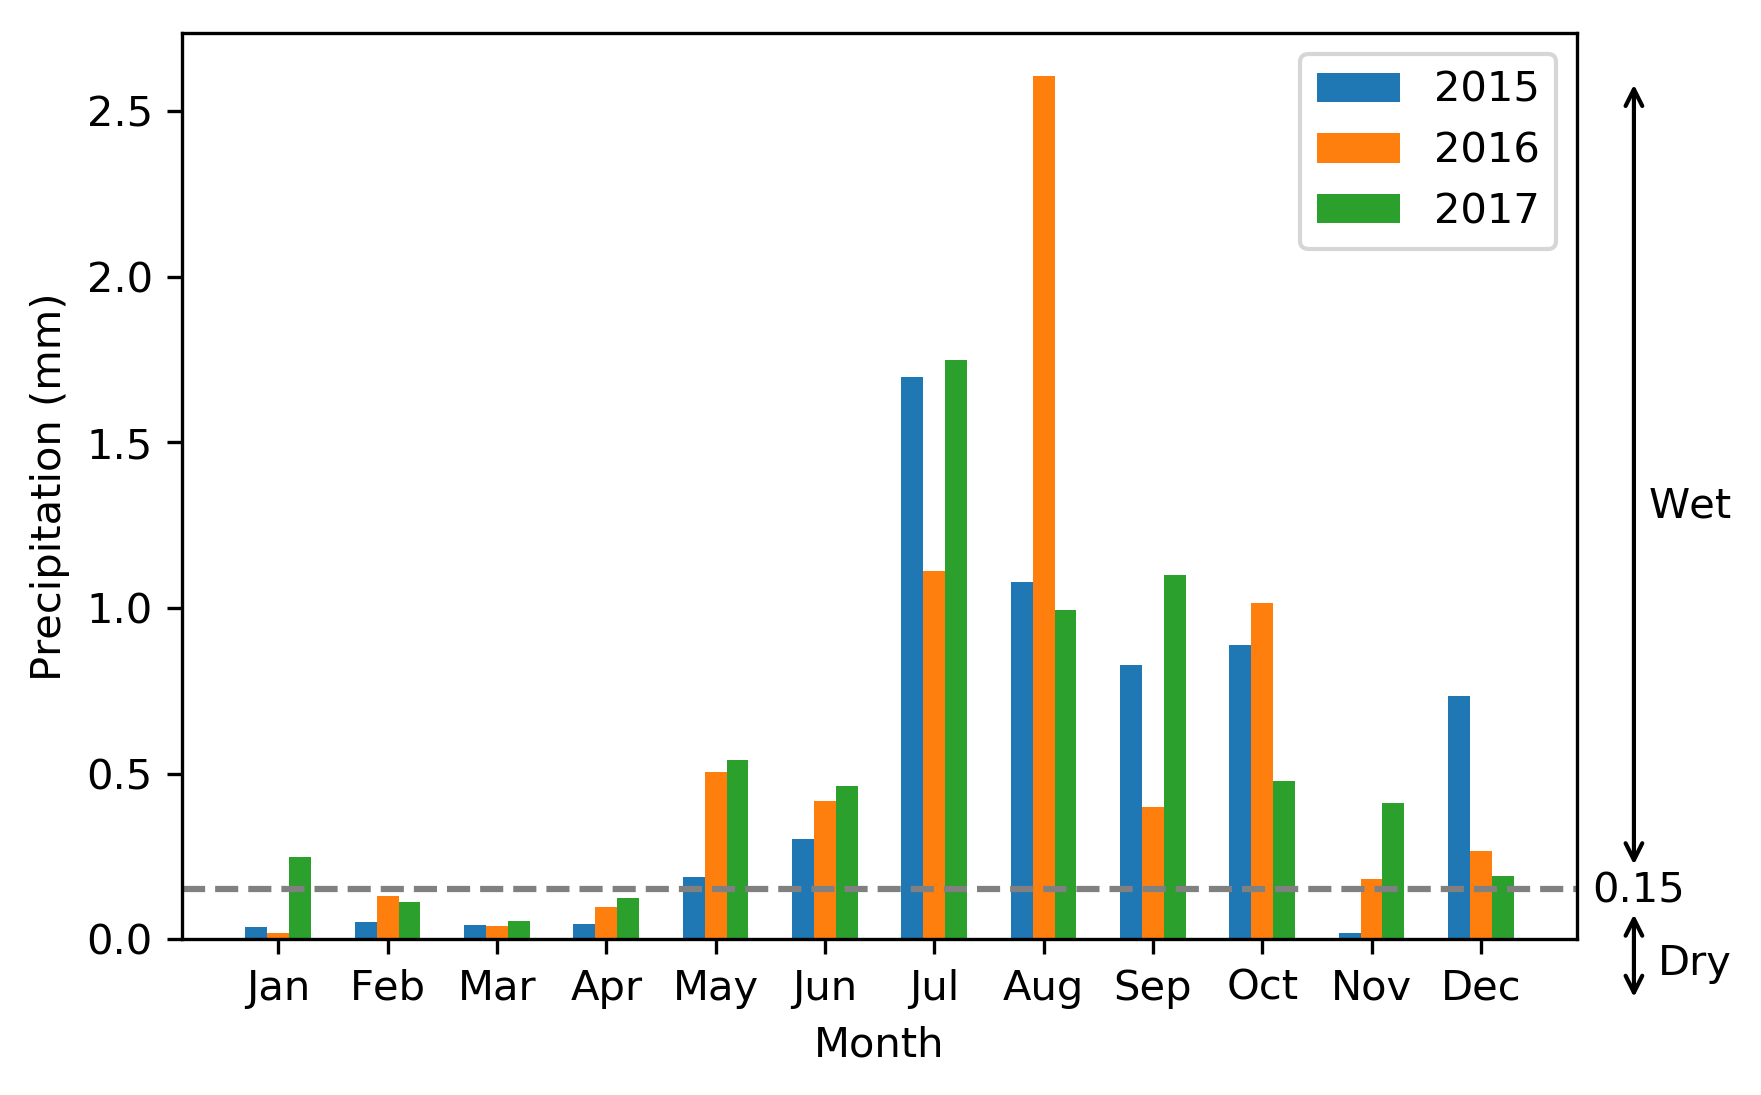
\includegraphics{figures/figure_ave_precip.PNG}}
  \caption{Wet and dry season defined by the average precipitation per month from 2015 to 2017}
\label{figure_ave_precip}
\end{figure}

% Wet and dry season defined by the average precipitation per month from 2015 to 2017
% \label{figure_ave_precip}


\subsubsection{Disrupted Day}

It is important to note that when defining disrupted days in respect to traffic, there are two factors to consider. First, it has been established by analyzing the traffic trends that increase in traffic mostly occur around 6:00. Thus, to observe the effects of prolonged rainfall to traffic, the instances of precipitation during the evening should be disregarded as its effect is more likely to decay when it is expected to effect during the morning. In the following experiments, only weather instances from 0:00 to 21:00 will be observed.

Second, only working days are considered as these are the days when traffic is significantly dynamic, hence disruption on its pattern can be observed. Given this, similar in our previous experiments in traffic, holidays and suspensions are considered as outliers as its traffic pattern would be inconsistent with its usual working day pattern.

Meanwhile, for weather, a threshold should be made with respect to the number of intervals per day. Given that a day is defined by 96 15-minute intervals, a cumulative minimum of 28 intervals or 7 hours of rain condition will be set as the threshold in classifying a disrupted day.

With these criteria set, a total of 69 disrupted days have been identified, in which 44.92% came from working days under the typhoon. As expected, the majority of these are taken from the wet season, more specifically 94.20% of it.

\subsection{Traffic Disruption}
Comparing the autocorrelation between dry and wet season, it could be observed that the daily seasonality of traffic becomes less evident during the wet season (see Figure \ref{figure_autocorr_traffic_season}). This could be due to the abundance of precipitation, disrupting the normal pattern of traffic.


\begin{figure}[h] 
\centering
    \centering
      \captionsetup{justification=centering}
    \subfloat[Dry Season]{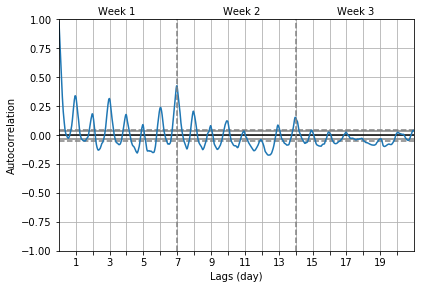
\includegraphics[width=0.5\textwidth]{figures/figure_traffic_autocorr_dryseason.png}\label{figure_traffic_autocorr_dryseason}}
    \hfill
    \subfloat[Wet Season]{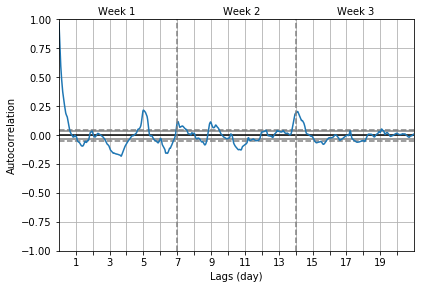
\includegraphics[width=0.5\textwidth]{figures/figure_traffic_autocorr_wetseason.png}\label{figure_traffic_autocorr_wetseason}}
    \caption{Autocorrelation of traffic comparing the daily and weekly seasonality per season showing that its pattern is disrupted during the wet season}
    \label{figure_autocorr_traffic_season}
\end{figure}

% Dry Season
% \label{figure_traffic_autocorr_dryseason}

% (b) Wet Season
% \label{figure_traffic_autocorr_wetseason}

% Autocorrelation of traffic comparing the daily and weekly seasonality per season showing that its pattern is disrupted during the wet season
% \label{figure_autocorr_traffic_season}

To verify this, we compare one observation of traffic (a week before Typhoon Goring) with its previous week (on the week of the typhoon). Basing from the seasonality of traffic, it is expected that the current traffic pattern would be similar to its previous week (see Figure \ref{figure_traffic_disrupted}). However, visualizing the current traffic pattern with its previous week, it could be observed that there is a significant increase in traffic as compared with the previous week of traffic.

\begin{figure}[h] 
\centering
  \scalebox{.85}{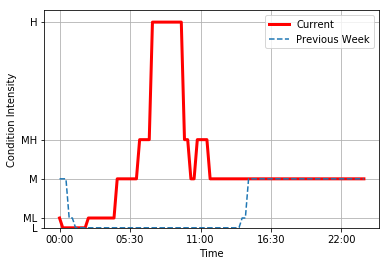
\includegraphics{figures/figure_traffic_disrupted.png}}
  \caption{Comparison between the current traffic and its previous week pattern showing a disrupted pattern}
  \label{figure_traffic_disrupted}
\end{figure}

% Comparison between the current traffic and its previous week pattern showing a disrupted pattern
% \label{figure_traffic_disrupted}












































\section{Correlation Analysis}
\subsection{Correlation of Engineered Traffic Features with Traffic Condition}

\subsubsection{Mean of Previous Weeks}
As the weekly seasonality of traffic remains consistent in both dry and wet season, the previous weeks could be potentially used to override the disrupted pattern of the previous week of a specific observation. In identifying this pattern, the mean of the traffic for the past weeks are taken. Correlating against the previous day and previous week seasonality, we could immediately observe an increase in the strength of its relationship with the present traffic (see Table \ref{table_corr_nomean_vs_mean}).



\begin{table}[]
\centering
\caption{Comparison between previous day and week traffic with the traffic mean 4-weeks-ago showing significant increase in strength in its relationship}
\label{table_corr_nomean_vs_mean}
\begin{tabular}{|l|r|}
\hline
                                                                            & \textbf{Correlation value} \\ \hline
\textbf{\begin{tabular}[c]{@{}l@{}}Previous Day\\ Traffic\end{tabular}}     & 0.265                      \\ \hline
\textbf{\begin{tabular}[c]{@{}l@{}}Previous Week\\ Traffic\end{tabular}}    & 0.282                      \\ \hline
\textbf{\begin{tabular}[c]{@{}l@{}}Traffic Mean\\ 4-weeks-ago\end{tabular}} & 0.391                      \\ \hline
\end{tabular}
\end{table}

% Comparison between previous day and week traffic with the traffic mean 4-weeks-ago showing significant increase in strength in its relationship
% \label{table_corr_nomean_vs_mean}

Further experimenting with the strength of its relationship, we examined the correlation of from 2-weeks-ago traffic up to 7-days-ago traffic (see Table \ref{table_corr_mean}). From this, we have identified the ideal range to be 6 weeks ago, as the relationship already starts to fade when 7 weeks ago is reached. Interestingly, the traffic mean 2-weeks-ago has a weaker relationship to the current traffic than the succeeding number of weeks. This could be due to the fact that at 2 weeks, there exist only the traffic of the previous week and the traffic 2 weeks ago. Considering the observation at the previous week is disrupted, then the effect of it is not minimized as you’re only aggregating it against one more value.



\begin{table}[]
\centering
\caption{Comparison of correlation values on the traffic mean of a range of weeks}
\label{table_corr_mean}
\begin{tabular}{|l|r|}
\hline
\textbf{\begin{tabular}[c]{@{}l@{}}Traffic Mean\\ N-weeks-ago\end{tabular}} & \textbf{Correlation value} \\ \hline
\textbf{2}                                                                  & 0.293                      \\ \hline
\textbf{3}                                                                  & 0.327                      \\ \hline
\textbf{4}                                                                  & 0.391                      \\ \hline
\textbf{5}                                                                  & 0.399                      \\ \hline
\textbf{6}                                                                  & \textbf{0.418}             \\ \hline
\textbf{7}                                                                  & 0.411                      \\ \hline
\end{tabular}
\end{table}


% Comparison of correlation values on the traffic mean of a range of weeks
% \label{table_corr_mean}

To verify this finding, Figure \ref{figure_traffic_mean_2weeks_vs_6weeks} illustrates an observation from an undisrupted time span, comparing the similarity of the current pattern with the traffic mean 6 weeks ago and 2 weeks ago. From this, it could be observed how close the current pattern with the mean of the traffic 6 weeks ago, specifically from 6:00 to 13:00.


\begin{figure}[h] 
\centering
  \scalebox{.90}{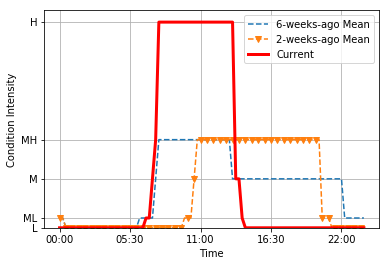
\includegraphics{figures/figure_traffic_mean_2weeks_vs_6weeks.png}}
  \caption{One-day visualization of the relationship between the current traffic and the mean of the traffic 6 weeks ago and 2 weeks ago}
  \label{figure_traffic_mean_2weeks_vs_6weeks}
\end{figure}


% One-day visualization of the relationship between the current traffic and the mean of the traffic 6 weeks ago and 2 weeks ago
% \label{figure_traffic_mean_2weeks_vs_6weeks}

This observation holds true even in disrupted days. Figure \ref{figure_traffic_mean_2weeks_vs_6weeks_disrupted} shows an observation after a week of Typhoon Goring. It could be seen in this visualization that the 6-weeks-ago traffic mean appeared to be more similar to the pattern of the current traffic as compared with the 2-weeks-ago traffic mean. As mentioned earlier, this could be due to the fact that getting the mean of just two observations where one is disrupted may not be enough to capture the undisrupted relationship of the previous weeks of traffic.

\begin{figure}[h] 
\centering
  \centering
  \scalebox{.85}{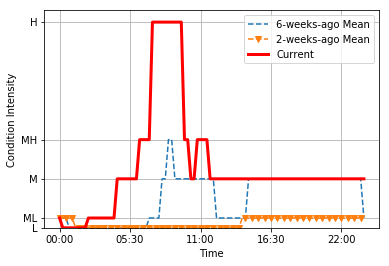
\includegraphics{figures/figure_traffic_mean_2weeks_vs_6weeks_disrupted.png}}
  \caption{One-day visualization of the relationship between the current traffic and the mean of the traffic 6 weeks ago and 2 weeks ago after a week of Typhoon Goring}
  \label{figure_traffic_mean_2weeks_vs_6weeks_disrupted}
\end{figure}


% One-day visualization of the relationship between the current traffic and the mean of the traffic 6 weeks ago and 2 weeks ago after a week of Typhoon Goring
% \label{figure_traffic_mean_2weeks_vs_6weeks_disrupted}

\subsection{Correlation of Immediate Traffic Features with Traffic Condition}

The data only describes the traffic condition per timestep and the seasonality of traffic. Although traffic has pattern, there are instances when a certain disruption in traffic may cause congestion build up. Therefore, considering how the immediate past traffic conditions may affect the current traffic condition can be considered as a factor for predicting traffic. Data  from the previous timestep can be used as a reference in predicting the current traffic condition. However, the change in traffic in a 15-minute timeframe may not be significant. As seen in Figure \ref{autocorr_whyRE}, autocorrelation reveals that a traffic condition is highly likely to reoccur every 15 minutes. In other words, the traffic condition of the previous time step is highly likely to be the traffic condition of the current time step. However, this does not capture the effects of sudden outliers to the build up or decay of traffic. Thus, it does not fully describe how the past traffic conditions might affect the current traffic condition. 


\begin{figure}[h] 
\centering
  \centering
  \scalebox{.85}{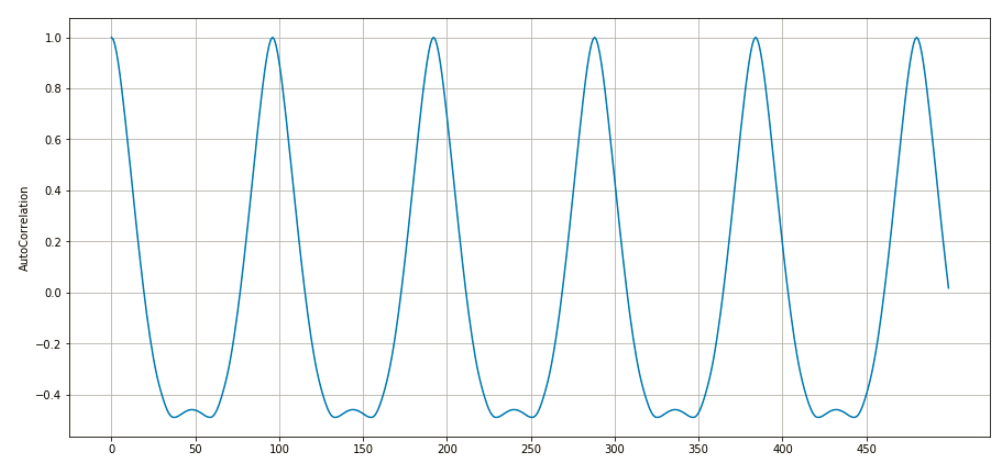
\includegraphics{figures/autocorr_whyRE.PNG}}
  \caption{Autocorrelation of traffic for working days}
  \label{autocorr_whyRE}
\end{figure}

% Autocorrelation of traffic for working days
% \label{autocorr_whyRE}

Generating rolling and expanding features based on a specific window size gives a bigger look as to what the current traffic might be based from the previous traffic conditions. Rolling and expanding window traffic features such as the mean, the minimum, and the maximum with window size  4, 8, 24, 48, and 96 were generated from the original traffic data. To summarize the possible effects of sudden changes in traffic, the mean of the past traffic conditions based on a window size was generated. Figure \ref{stDev} shows the standard deviation values of traffic for every window size. Standard deviation shows the variability or the distance of the data from the mean. From this, it can be observed that there is a rising pattern in the growth of the standard deviation as the window size increases. The low standard deviation of smaller window sizes signifies that there is only a little to no change in traffic condition within that time frame. Meanwhile, large window sizes like window 96 which yield a relatively larger standard deviation value of 0.03531 than of window 4, implies that the traffic conditions in a 1-day time frame are more varied or are more widely spread. With small window sizes, the values generated captures less of the trifle changes in traffic and gets more affected by outlier values which then results in a more generic information. However, as the window size increases, the effect of outlier values also get more neutralized because of the number of data considered, giving a broader summary of the past traffic. 

\begin{figure}[h] 
\centering
  \centering
  \scalebox{.85}{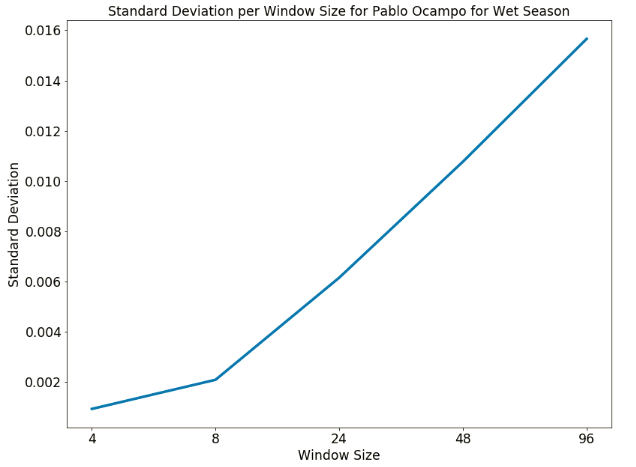
\includegraphics{figures/pocampo_stdev.PNG}}
  \caption{Standard Deviation of Traffic per Window Size for the Wet Season in Pablo Ocampo}
  \label{stDev}
\end{figure}

% Standard Deviation of Traffic per Window Size for the Wet Season in Antipolo
% \label{stDev}

The minimum and maximum features, on the other hand, reveals the range of x in the dataset. Being sensitive to outliers, they provide outlier detection when compared to the average value of that specific set of data. A big difference between the values of the minimum and the maximum signifies a large progression in traffic condition. Although as the window size used gets bigger, it becomes harder to determine whether the sudden change in traffic condition occurred just a few timesteps before or if it is because of a farther instance which may have less to no effect to the current traffic condition. 

\begin{figure}[h] 
\centering
    \centering
      \captionsetup{justification=centering}
    \subfloat[Original vs. Rolling]{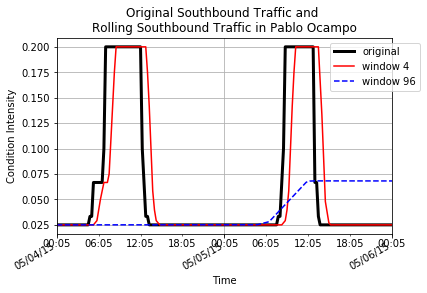
\includegraphics[width=0.5\textwidth]{figures/pocampo_rolling.png}\label{pocampo_rolling}}
    \hfill
    \subfloat[Original vs. Expanding]{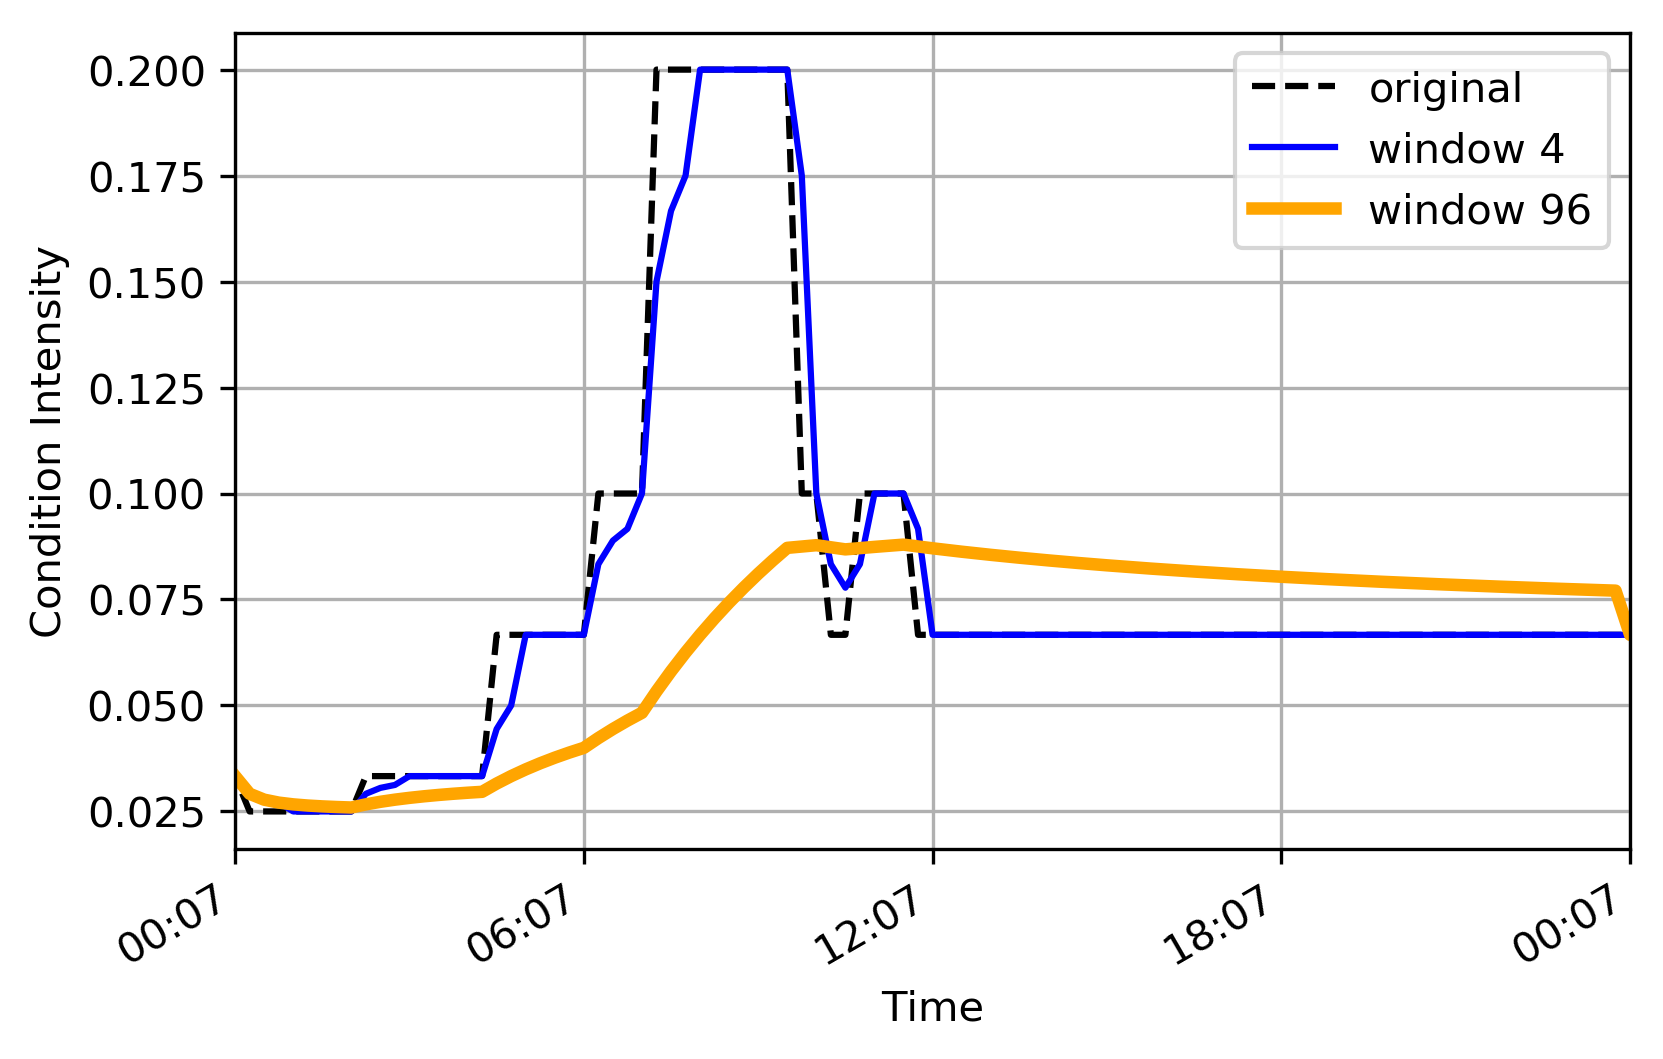
\includegraphics[width=0.5\textwidth]{figures/pocampo_expanding.png}\label{pocampo_expanding}}
    \caption{Comparison of Rolling and Expanding windows 4 and 96 to original Northbound traffic in Pablo Ocampo}
    % \label{figure_autocorr_traffic_season}
\end{figure}

\begin{figure}[h] 
\centering
  \centering
  \scalebox{.65}{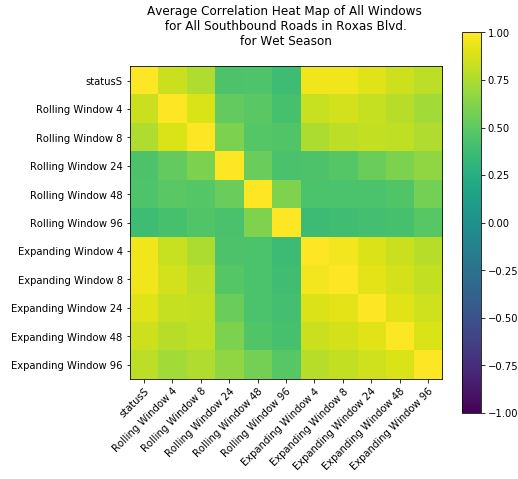
\includegraphics{figures/heatmap_roxas.JPG}}
  \caption{Average Correlation of Rolling and Expanding Mean to All Southbound Roads in Roxas Blvd.}
  \label{heatmap_roxas}
\end{figure}

Figure \ref{heatmap_roxas} shows the average correlation of southbound road segments of Roxas Boulevard per window size in relation to traffic for both rolling and expanding windows. On average, the original traffic has a strong relationship with rolling features having small window size, specifically window 4 with a correlation value of 0.7501. It is noticeable, however, that the strength of the relationship dwindles down as the window size increases. This reveals that although having a bigger window size means being able to capture various changes in traffic condition, it does not give importance to the most recent traffic conditions. Big changes in traffic conditions that occurred way back and may not have any effect on the current traffic are being considered. Thus, causing its misalignment to the original data. 

In the case of expanding windows, the strength of the relationship to the original traffic also decreases as the window size increases, albeit not so much as the rolling mean do. Looking into both graphs, the strength of the relationship given by window 4 for both rolling and expanding is distinctly stronger compared to the ones with larger window size. This might be because as mentioned earlier, traffic does not usually change significantly within a small window. Furthermore, a smaller window size means that its frequency of reverting back to the original value, making its generated value more accurate. Meanwhile, the farther from the past that it considers, the less it captures changes in traffic. This is shown in Figures \ref{pocampo_rolling} and \ref{pocampo_expanding}, where rolling and expanding at window 96 generalizes the high condition intensities into information that is no longer close to reality. Furthermore, the plodding decrease of correlation strength in expanding features as compared to rolling features is caused by limiting the number of windows that the feature grows to and considers and the restarting of its window size. Not limiting the window size growth of expanding features would produce values that are very far away from reality because it would consider every data from the previous days. It would contain values that consider data that are not relevant in predicting the future traffic.




\subsection{Correlation between Connected Road Segments}
To be able to identify if there is a direct relationship between connected road segments, we first perform an initial correlation on their traffic for all working days in one month. Figure \ref{figure_traffic_roxas_corr} illustrates the correlation heatmap of the traffic of road segments in Roxas Boulevard. From this, we could observe a consistent strong relationship between each road. 



\begin{figure}[h] 
\centering
    \centering
      \captionsetup{justification=centering}
    \subfloat[Southbound]{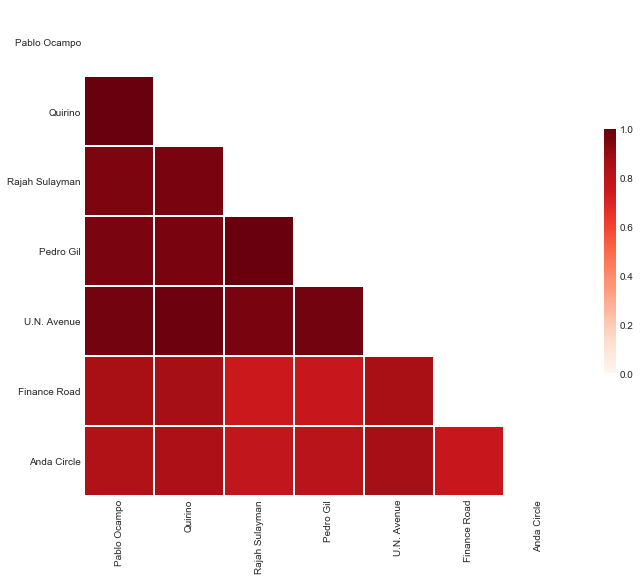
\includegraphics[width=0.5\textwidth]{figures/figure_traffic_roxas_sb_corr.png}\label{figure_traffic_roxas_sb_corr}}
    \hfill
    \subfloat[Northbound]{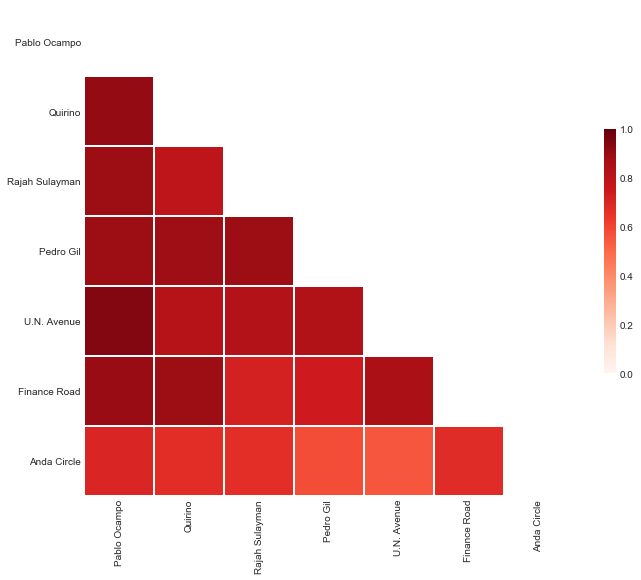
\includegraphics[width=0.5\textwidth]{figures/figure_traffic_roxas_nb_corr.png}\label{figure_traffic_roxas_nb_corr}}
    \caption{Correlation heatmap of traffic for both southbound and northbound of Roxas Boulevard}

    \label{figure_traffic_roxas_corr}
\end{figure}

This strong relationship remains true with the traffic for both southbound and northbound for Espana (see Figure \ref{figure_traffic_espana_corr}). Compared with Roxas Boulevard, however, there are certain road segments in Espana that have relatively weak relationship with its nearby road segments.


\begin{figure}[h] 
\centering
    \centering
      \captionsetup{justification=centering}
    \subfloat[Southbound]{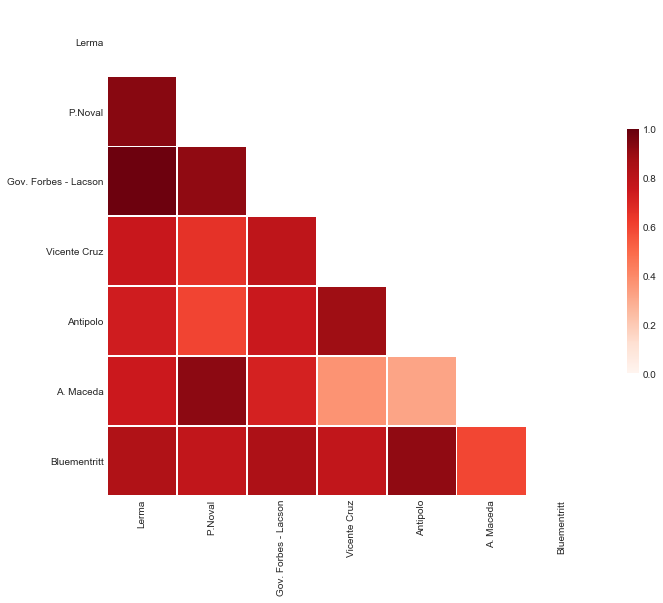
\includegraphics[width=0.5\textwidth]{figures/figure_traffic_espana_sb_corr.png}\label{figure_traffic_espana_sb_corr}}
    \hfill
    \subfloat[Northbound]{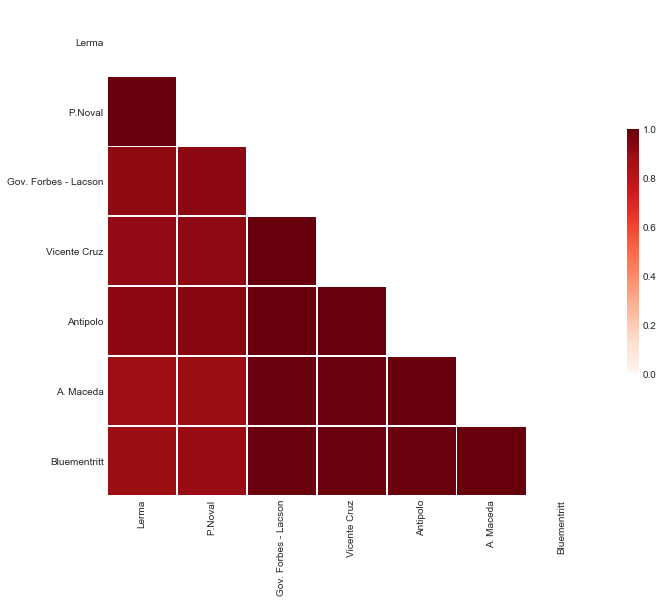
\includegraphics[width=0.5\textwidth]{figures/figure_traffic_espana_nb_corr.png}\label{figure_traffic_espana_nb_corr}}
    \caption{Correlation heatmap of traffic for both southbound and northbound of Espana}

    \label{figure_traffic_espana_corr}
\end{figure}


After analyzing the pattern of an individual road segment, we now analyze it as a part of a road. Exploring the working day traffic of all road segments in Roxas Boulevard in one month, it could be observed that there is an intensity relationship between these southbound road segments such that their peaks remains the same yet their intensity differs (see Figure \ref{figure_traffic_roxas}). This is also the case in the northbound of the road segments in Roxas Boulevard. The intense traffic of Pablo Ocampo is carried over to Quirino in a similar intensity yet continuously decays as we go further to Anda Circle.



 \pagebreak[4]
\begin{figure}[h] 
\centering
    \centering
      \captionsetup{justification=centering}
    \subfloat[Southbound]{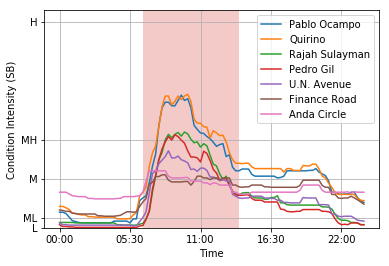
\includegraphics[width=0.5\textwidth]{figures/figure_traffic_roxas_sb.png}\label{figure_traffic_roxas_sb}}
    \hfill
    \subfloat[Northbound]{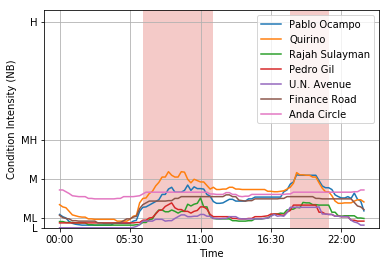
\includegraphics[width=0.5\textwidth]{figures/figure_traffic_roxas_nb.png}\label{figure_traffic_roxas_nb}}
    \caption{Daily average of all working days in one month in all road segments in Roxas Boulevard showing its intensity relationship}

    \label{figure_traffic_roxas}
\end{figure}




Likewise, in road segments of Espana, it follows a similar trend (see Figure \ref{figure_traffic_espana}). The intensity of the traffic at the northbound of Blumentritt rises as we approach Antipolo then decays as we go further to Lerma.


\begin{figure}[h] 
\centering
    \centering
      \captionsetup{justification=centering}
    \subfloat[Southbound]{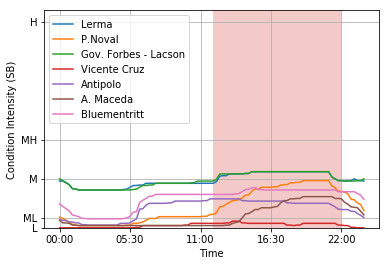
\includegraphics[width=0.5\textwidth]{figures/figure_traffic_espana_sb.png}\label{figure_traffic_espana_sb}}
    \hfill
    \subfloat[Northbound]{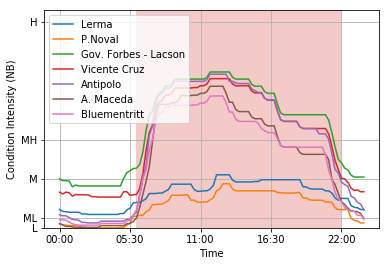
\includegraphics[width=0.5\textwidth]{figures/figure_traffic_espana_nb.png}\label{figure_traffic_espana_nb}}
    \caption{Daily average of all working days in one month in all road segments in Espana showing its intensity relationship}

    \label{figure_traffic_espana}
\end{figure}

































 \pagebreak[4]
\section{Predicion Model Evaluation}

\subsection{Traffic-Only Model}
As seen in Figure \ref{fig:tom_diff_feat_combi} the inclusion of the information about working days and peak hours for all road segments improved the performance of the model by only 22\% having originally an RMSE of 0.167 which improved to 0.113. As discussed earlier on the trend and patterns of traffic, though there is a difference between the trends of working days and non-working days, light and moderate traffic are most frequent in both trends in the majority of the road segments. This implies that the mean traffic condition intensity for both working and non-working days are similar. This similarity attributes to the small improvement in the prediction. Furthermore, including rolling and expanding window features for traffic significantly improved the prediction by around 53\%, from having an RMSE of 0.129 to 0.061 by window 4. Rolling and Expanding window features present a generalized information regarding the trend of the immediate past traffic. As discussed earlier, average traffic does not change significantly within a small window. Moreover, increasing the window size of both features As such, the performance of the model decreases as the window increases. 

\begin{figure}[h]
  \centering
  \captionsetup{justification=centering}
  \scalebox{.65}{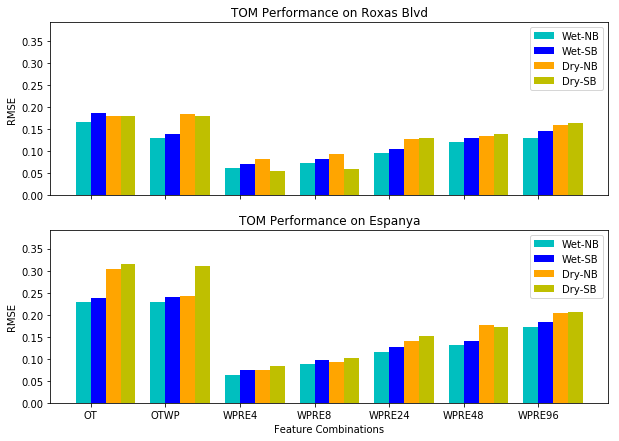
\includegraphics{tom_diff_feat_combi.PNG}}
  \caption{Comparison between performance of TOM on Roxas Boulevard and Espana using different feature combinations}
  \label{fig:tom_diff_feat_combi}
\end{figure}

To evaluate if the model can successfully identify the trends present for each road segment, and its ability to predict its traffic, the performance of the model using OTWP or Original Traffic with the addition of work day and peak hours was observed. Results of this evaluation are illustrated in Figure \ref{fig:tom_feat_combi_road}. The model predicted the southbound traffic of España during the wet season quite well, having a mean RMSE of 0.095 compared to the other. However, this is because of the diversity of the southbound traffic of España during the wet season, having a moderate traffic congestion majority of the time. Given only data of the previous day’s traffic, and information on work day and peak hours, the model cannot easily model the sudden peaks and traffic reports on heavy traffic. Additionally, given the percentage of the report on heavy traffic congestion of the data, having only 10.584\% during the working days, and 0.301\% during the non-working days, the model lacks knowledge on modeling expected heavy traffic. 

\begin{figure}[h]
  \centering
  \captionsetup{justification=centering}
  \scalebox{.55}{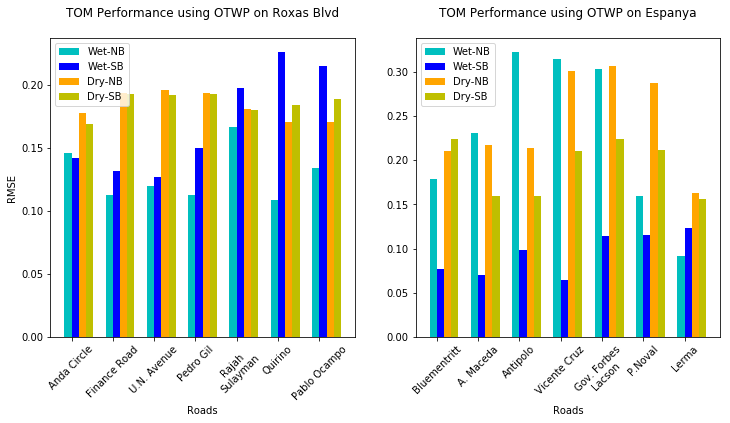
\includegraphics{tom_feat_combi_road.PNG}}
  \caption{Performance of TOM on Roxas Boulevard and España using OTWP traffic feature combination}
  \label{fig:tom_feat_combi_road}
\end{figure}
 

Disrupted days refer to the period in time wherein the trend of traffic goes out of its normal trend. Traffic that goes out of its normal trend is most expected during days that have  heavy rainfall, or periods when typhoons are present. Figure \ref{fig:TOM_normal_disrption_pocampo_antipolo_wet} illustrates the prediction of TOM for traffic condition intensity for road segments of Pablo Ocampo and Antipolo during the wet season for the month of September. Normal trend includes the week of September 20 to 26, and the disrupted trend includes the week of September 6 to 12, both weeks include weekday and weekend. The period of disruption, specifically September 11 to 12, there are 40 and 56 instances of heavy rainfall, respectively. The actual traffic during the period of disruption transition from heavy traffic to to moderate traffic in just a small time interval, unlike normal transitions. The model successfully predicts the abrupt transition of low traffic to high traffic for both normal and disrupted periods. However, the model delays in predicting the abrupt transitions from high traffic to moderate traffic, and moderate traffic to moderately high traffic. These difficulty in prediction can be attributed to the few instances where these abrupt transitions are present. As seen, normal trends do not often include these abrupt transitions. 

\begin{figure}[h]
  \centering
  \captionsetup{justification=centering}
  \scalebox{.65}{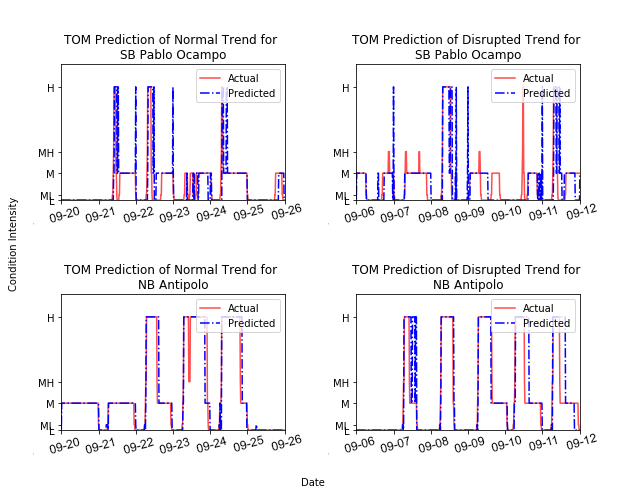
\includegraphics{TOM_normal_disrption_pocampo_antipolo_wet.PNG}}
  \caption{TOM Prediction for Normal (left) and Disrupted (right) trends for Pablo Ocampo and Antipolo}
  \label{fig:TOM_normal_disrption_pocampo_antipolo_wet}
\end{figure}

\subsection{Weather-Only Model}
Given the weak relationship between weather variables with traffic, the model could only predict traffic about 80 to 84\% after using weather variables for input as compared to using past traffic that can predict traffic by 90\%. Furthermore, the model’s performance did not improve significantly with different combinations (see Figure \ref{fig:wom_diff_feat_combi}) of weather variables having changes in error ranging from only 0.001 to 0.003. Weather variables were found to have a low correlation, ranging from 0.01 to 0.3 with respect to the traffic condition intensity. Including and removing redundant variables, and other low correlated variables did not have a significant effect on the prediction. 

\begin{figure}[h]
  \centering
  \captionsetup{justification=centering}
  \scalebox{.55}{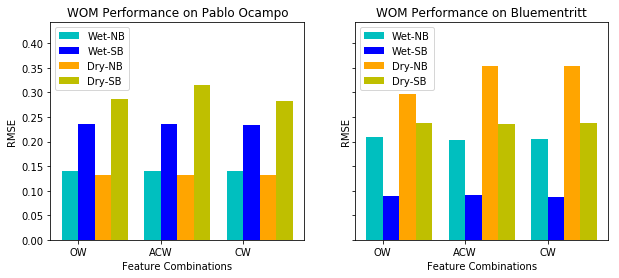
\includegraphics{wom_diff_feat_combi.PNG}}
  \caption{Performance of WOM on Pablo Ocampo and Antipolo using weather feature combinations}
  \label{fig:wom_diff_feat_combi}
\end{figure}


Figure \ref{fig:wom_feat_combi_roads} illustrates the performance of WOM following OW feature combination for all road segments of España and Roxas Blvd. For predicting Roxas Blvd road segments using WOM, the model predicts traffic better during the wet season. Additionally, WOM predicts northbound well for most road segments in Roxas Blvd during the wet season. Northbound traffic for these roads is less diverse, meaning that traffic majorly consists of low to moderate traffic, with only a few instances of abrupt transitions from these conditions to heavy traffic. Given these, WOM could not learn the pattern of these transitions given the few instances. In predicting the traffic of Roxas Blvd road segments during the dry season, the WOM could only predict 70\% of the traffic for the northbound of all road segments except Pedro Gil having an average RMSE of 0.250. 

As for predicting España Road segments using WOM, the model predicts southbound traffic of all roads during the wet season better. The WOM got an average RMSE of 0.329 in predicting northbound traffic for road segments Bluementritt to P. Noval, compared to predicting its southbound counterpart having an average RMSE of 0.116. Like Roxas Boulevard road segments, the southbound traffic of España road segments is less diverse, consisting mostly of low to moderate traffic.

For both roads of Roxas Boulevard and Espana, WOM could better predict the bound of a road segment with less diverse traffic, in which instances where traffic abruptly transitions to another traffic condition is not present. Moreover, WOM cannot predict fully traffic during the dry season, wherein weather, most especially rainfall, is less expected that can affect traffic fully. 


\begin{figure}[h]
  \centering
  \captionsetup{justification=centering}
  \scalebox{.55}{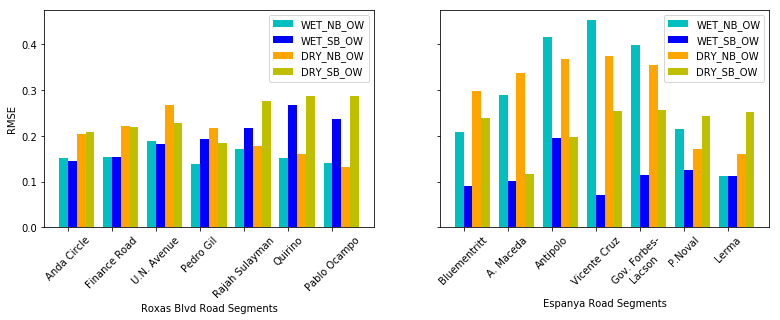
\includegraphics{wom_feat_combi_roads.PNG}}
  \caption{Performance of WOM using OW weather feature combination for all road segments}
  \label{fig:wom_feat_combi_roads}
\end{figure}

Given only temporal information and the weather variables to predict the current traffic condition intensity, and adding the fact that there is a small distribution of moderately high to high traffic in the data, the model could only predict low to moderate traffic successfully. Figure \ref{fig:WOM_normal_disrption_pocampo_antipolo_wet} illustrates the prediction of WOM for traffic condition intensity for road segments of Pablo Ocampo and Antipolo during the wet season for the month of September. WOM, however, predicted the transition of traffic from Low Traffic to either moderately low and moderate traffic well. WOM could predict the length of consistent traffic for both normal and disrupted periods. 

\begin{figure}[h]
  \centering
  \captionsetup{justification=centering}
  \scalebox{.65}{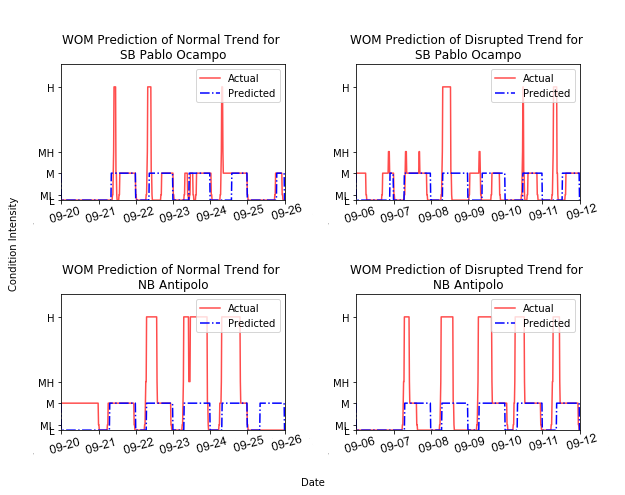
\includegraphics{WOM_normal_disrption_pocampo_antipolo_wet.PNG}}
  \caption{WOM Prediction for Normal (left) and Disrupted (right) trends for Pablo Ocampo and Antipolo}
  \label{fig:WOM_normal_disrption_pocampo_antipolo_wet}
\end{figure}


\subsection{Fusion Analysis}
In analyzing the effectiveness of including weather as a factor in predicting traffic, the road segments which are strongly correlated with weather variables, and are more dynamic are selected in further analysis. These roads are southbound of Pablo Ocampo and northbound of Antipolo. The final results displayed are the average of the results of these two road segments.

\begin{table}[]
\begin{tabular}{|l|r|r|r|r|r|r|}
\hline
\multirow{2}{*}{\textbf{Fusion Techniques}} & \multicolumn{2}{c|}{\textbf{OTWP + OW}}                                & \multicolumn{2}{c|}{\textbf{WPRE 4 + OW}}                              & \multicolumn{2}{l|}{\textbf{WPRE 96 + OW}}                             \\ \cline{2-7} 
                                            & \multicolumn{1}{c|}{\textbf{RMSE}} & \multicolumn{1}{l|}{\textbf{MAE}} & \multicolumn{1}{c|}{\textbf{RMSE}} & \multicolumn{1}{l|}{\textbf{MAE}} & \multicolumn{1}{l|}{\textbf{RMSE}} & \multicolumn{1}{l|}{\textbf{MAE}} \\ \hline
\textbf{Traffic-Only Model}                 & 0.314                              & 0.148                             & 0.084                              & 0.011                             & 0.234                              & 0.090                             \\ \hline
\textbf{Weather-Only Model}                 & 0.328                              & 0.149                             & 0.328                              & 0.149                             & 0.328                              & 0.149                             \\ \hline
\textbf{DBN Feature Fusion}                 & 0.353                              & 0.193                             & 0.100                              & 0.019                             & 0.282                              & 0.122                             \\ \hline
\textbf{DBN Decision Fusion}                & 0.334                              & 0.185                             & 0.078                              & 0.014                             & 0.206                              & 0.085                             \\ \hline
\textbf{RNN Decision Fusion}                & 0.068                              & 0.054                             & 0.171                              & 0.131                             & 0.103                              & 0.085                             \\ \hline
\textbf{WA Decision Fusion}                 & 0.365                              & 0.198                             & 0.287                              & 0.174                             & 0.292                              & 0.202                             \\ \hline
\end{tabular}
\caption{Comparison between Prediction Models and Fusion Models}
\label{table:fusion_results}
\end{table}

The model performed better with fusing traffic and weather in the decision level than at the feature level. However, the difference between fusing in these levels is small, having the difference in RMSE of only 0.019. Predicting traffic considering both traffic and weather at the same time may weigh down the prediction of traffic because of the influence of weather. As discussed in early analysis of the weather data, it was found that weather variables do not have a derivable relationship with traffic. Adding weather features together with traffic adds more complexity to the model, adding more insignificant patterns to the learning, decreases the performance of the model to predict traffic. On the other hand, in fusing at the decision level, the traffic predicted by TOM does not have influence with weather, thus, minimizing the weights in predicting traffic. 

Figure \ref{fig:dbn_comp_pocampo} illustrates the differences of performance between DBN models. Including weather as a factor in predicting traffic improved the final predicting as seen in the results of fusing in the decision level. This improvement is significantly evident in the performance of the model after using predictions of TOM and WOM that used OTWP traffic features, and OW weather features, respectively. The prediction improved by 71\%, from having an RMSE of 0.084 to 0.024. As for using predictions of TOM and WOM that used WPRE4 traffic features and OW weather features, the predictions improved by 16\%. A reason behind only the small improvement is because of the consideration of rolling and expanding features at window 96, or within the current day. The window may have consisted instances of disruption that may have been generalized by the averaging traffic within 96 windows. Additionally, there is a small number of instances of heavy traffic that assists the rolling and expanding features in generalizing the traffic within said window. 

In observing the performance of the model that uses the OTWP traffic features and OW weather features, the performance of WA is close to the DBN Feature and Decision Fusion model. The prediction of the TOM and WOM using OTWP and OW respectively are close to each other, having only a difference of 0.014. As such, DBN Feature and Decision Fusion, as with WA, could only predict traffic close to its inputs. However, considering the immediate past traffic, specifically considering the generalized past traffic of 1 hour and 1 day ago, may have improved the performance of fusing at both feature and decision levels with DBN, but fusing with WA fails to improve the prediction. WA cannot predict traffic in consideration of immediate past traffic features because of how it computes its weights through regression and averages the weighted inputs. WA computes its weights by computing the equation of the line of the data, specifically the predicted traffic for TOM and WOM. Given that the data is not linear, and that data is categorical, only having 5 values that denote the condition intensity, the generated line either have x or y-axis close to 0, generating weights that cannot fully describe the data. Moreover, WA averages the two predictions of TOM and WOM respectively, wherein TOM is significantly different than WOM. Thus, WA considers the outlier and generates an inaccurate prediction. Because of such performance, WA is not considered in further experiments. 

RNN outperforms DBN, and other fusion algorithms by 74\%. RNN is implemented as an LSTM, or a long short-term memory, compared to DBN which is implemented as a regressor and a classifier. Because of RNN’s power of long short-term memory, it can use their internal memory to process a sequence of inputs, successfully extracting ordered patterns. 

\begin{figure}[h]
  \centering
  \captionsetup{justification=centering}
  \scalebox{.65}{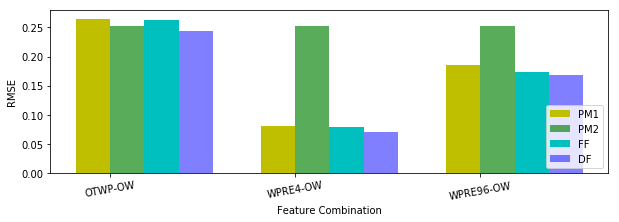
\includegraphics{dbn_comp_pocampo.PNG}}
  \caption{Comparison of DBN model in predicting the southbound of Pablo Ocampo for the wet season}
  \label{fig:dbn_comp_pocampo}
\end{figure}


The implemented model could predict normal trends of traffic. However, disrupted traffic trends defined in the discussion of the traffic and weather data cannot be accurately predicted. A reason behind the difficulty in prediction is the small number of instances of disruption in the training dataset. There is only a small number of instances of moderately heavy to heavy traffic within the wet season of the training dataset. Another reason may be because of the instances when disruptions in weather were present until the weekends when traffic is least expected. For example, for September 11 to 14 when typhoon Ineng was present, extends from a Friday until Sunday. The model also has a difficulty in predicting traffic using only weather features because of the weak relationship between these variables. For visualization purposes, the final prediction of traffic condition  intensity of Pablo Ocampo and Antipolo is illustrated in \ref{fig:final_prediction}.

\begin{figure}[h]
  \centering
  \captionsetup{justification=centering}
  \scalebox{.65}{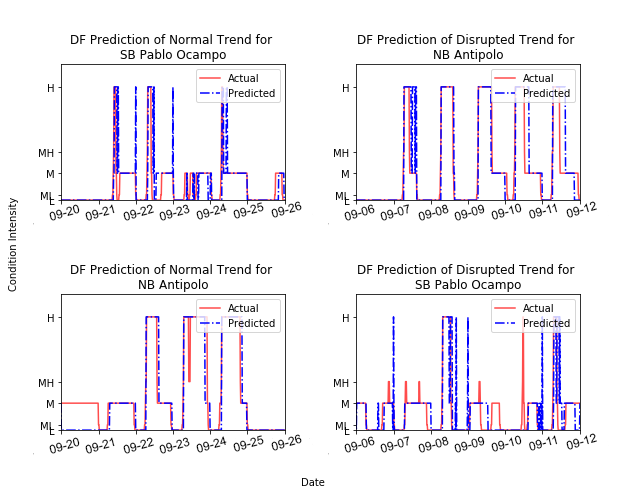
\includegraphics{final_prediction.PNG}}
  \caption{Final Prediction for Normal (left) and Disrupted (right) trends for Pablo Ocampo and Antipolo using DBN Decision Fusion}
  \label{fig:final_prediction}
\end{figure}



\subsection{Sensitivity Analysis}
To analyze the effectiveness of including weather as a factor in predicting traffic, the southbound traffic of Pablo Ocampo were selected. The final results displayed are the average of the results of these two road segments.

\subsubsection{Traffic-Only Model}

\begin{figure}[h]
  \centering
  \captionsetup{justification=centering}
  \scalebox{.65}{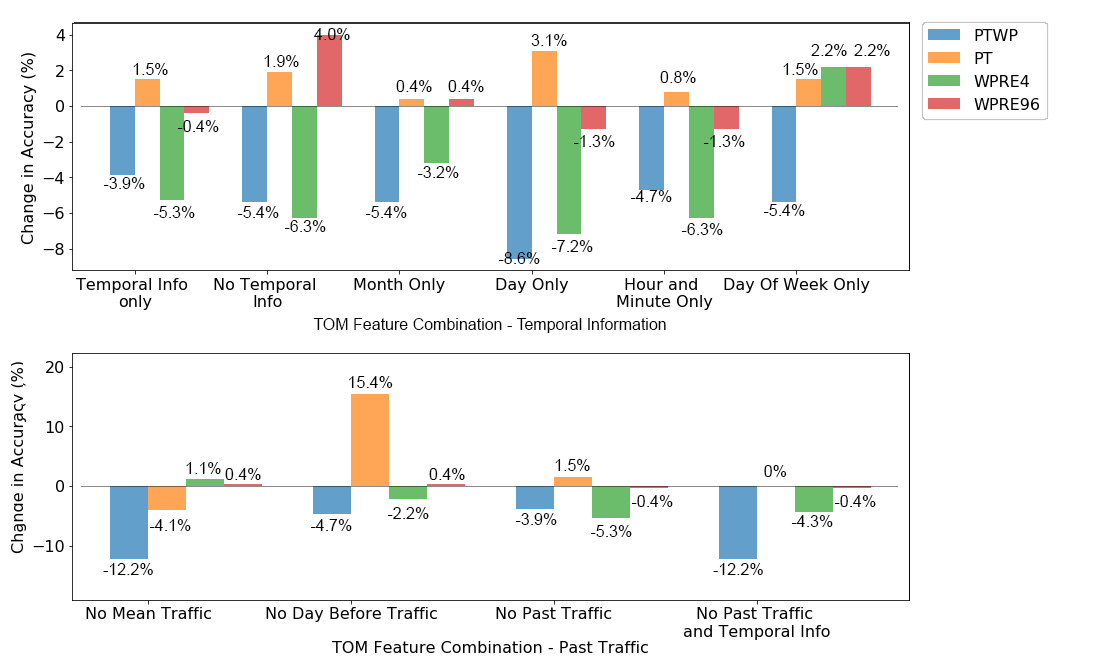
\includegraphics{TOM_sensitivity.PNG}}
  \caption{Sensitivity of TOM with different feature combinations}
  \label{fig:TOM_sensitivity}
\end{figure}

Evaluation of the sensitivity of TOM is illustrated in \ref{fig:TOM_sensitivity}. It has been discussed in the early sections in evaluating TOM that the inclusion of work day and peak hour variables result in a 22\% improvement in performance. The removal of temporal information decreased the performance from 3.9 to 8.6\% when used with work day and peak hour. Not one temporal information variable increase the accuracy of the base which used all the temporal information, and all past traffic features. However, without the work day and peak hour, removal of the temporal information seems to have increased the performance, but only by 1 to 3\%. Results show that temporal information, when used with working day and peak hour variables without past traffic information, decreases the performance by 4\%. Moreover, each variable excluding the $Day$ variable is independent of each other as seen by the change of accuracy when using only Month, Hour and minute, or day of the week. Using the day variable without the support of other temporal information have decreased the performance by 8.6\%. Results show that traffic does not have any pattern with the $Day$ variable. As for the use of temporal information without working day and peak hour, the model performed better. Working day and peak hour variables show a generalized information of traffic at a specific time period. Without this information, the temporal information instead gives information on the traffic such as what hours or day of the week is there heavy traffic condition intensity. 

Looking into the effect of the past traffic feature when used with the working day and peak hour, using either the mean of traffic 6 weeks ago, and a day before did not affect the performance, only having differences of 0.03\%. However, There is a significant change when work day and peak hours are not used. In using only the traffic a day before, the performance decreased by 4.1\%. Using the traffic 6 weeks ago significantly increased the performance by 15.4\%. Results show that the base model for OT that used all the past traffic features of a day and 6 weeks ago and all temporal information without workday and peak hour, gets most of its prediction bases from the general traffic 6 weeks ago. This shows that this variable has great importance in predicting traffic when working day and peak hours are not used.  

\begin{figure}[h]
  \centering
  \captionsetup{justification=centering}
  \scalebox{.65}{\includegraphics{pm1-pm2-df-changes.PNG}}
  \caption{Change in performance in different feature combinations}
  \label{fig:pm1-pm2-df-changes}
\end{figure}

\subsubsection{Decision Fusion Model}

The base model for evaluating the fusion between using the different prediction models, and fusion models is the Traffic-Only for OTWP feature combination. As discussed in the Fusion Analysis, considering the weather prediction in fusing at decision level resulted in a 14\% improvement in performance. However, in evaluating the performance of the weather in predicting traffic, weather only contributed about 27\% of the prediction. As mentioned in earlier discussions, traffic data mostly comprises of moderate traffic condition intensity reports. Additionally, periods where there is a disruption in weather in which traffic is expected lies in weekends when traffic is least expected. The data does not completely represent the relationship between weather and traffic, thus resulting in the small weight in prediction. 





































 
                                   \chapter{Conclusion}

Urban centers have long-since been fighting the natural occurrence of traffic congestion in the past decades. To help solve this problem, several traffic models were already developed while also considering weather as an effect. However, these models were not designed and tested in places with substandard drainage systems and poor road management. This research aims to adapt a weather-aware traffic model to cater these places. In this paper, analysis on the patterns of traffic and weather data were explored through correlation analysis. Features were also extracted to gain more insights as to what variables have a relationship with traffic congestion. An existing traffic model using DBNs and data fusion techniques was adapted to predict the traffic congestion in selected roads in Manila. Different experiment settings were done to show how different traffic and weather features affect the traffic prediction. 

Analysis show that patterns and trends are still evident even in urban centers where disruptions in traffic and weather are present. Additionally, extracting information from the categorical data of traffic congestion is possible and can be quite insightful. In evaluating the model in predicting future traffic, results show that using the immediate past traffic is insightful and bears importance in decision making. Results also show that fusing at decision-level improves accuracy in prediction better than feature-level. Moreover, though DBNs bear the ability to extract patterns, RNNs outperforms DBN in extracting the patterns of time-series data.
 
                                     \chapter{Future Works}

%%%% REAL TIME DATA COLLECTION %%%%
Using historical data is a good and common entry for data-driven researches. However, in the case of traffic, it is better to consider real-time information to predict future traffic conditions. In the event that something unexpected happens, such as road accidents or just-closed lanes, the historical traffic data may not be as useful as it is. Sudden events may also include typhoon warnings, which has no annual pattern and cannot be be easily predicted. With historical traffic and weather data combined with real-time information, future traffic predictions may become more accurate.

%%%% SOCIAL MEDIA REPORTS %%%%
Considering traffic reports in social media may also be an additional feature in the model. Social media platforms such as Twitter and Facebook allows people to let out their frustrations including everyday problems such as road traffic. One study \shortcite{gu2016twitter} retrieves real-time traffic information by crawling, processing, and filtering public tweets to detect road traffic incidents using natural processing language techniques. Using this as an added feature in the model may boost its accuracy. 

%%%% ROAD CATASTROPHES (accidents, constructions, closed) %%%%
Unpredicted road catastrophes also contribute to traffic congestion, including road accidents, road constructions, and recently-closed lanes. Car accidents block the roads, which then hinder other vehicles to efficiently pass through, causing heavy traffic jam \shortcite{wang2009impact}. Road constructions such as building of bridges, expanding the roads, fixing the water pipes underneath the roads, among others, also tend to increase traffic congestion, especially if there is no notice beforehand. The sudden closing of a road may also contribute to traffic jams, since it disrupts the normal flow of traffic. Studying these kinds of road catastrophes may be helpful in achieving a better traffic prediction. Data may be collected as historical data or using real-time information.

%%%% FLOOD %%%%
In urban places where drainage systems are not properly managed or road infrastructures are not properly built and maintained, the amount of rain accumulating on the roads may increase traffic congestion as vehicles have difficulty moving forward. It is worse on places where adverse weather conditions such as typhoons bring heavy rains, which then causes immense flooding if the rain is not properly drained. Although the existing application Waze allows drivers and passengers to report flooding incidents in the roads, Waze does not use these reports in learning and predicting future traffic conditions. In future works, considering the height of flood as a contributing factor may help the model in predicting future traffic condition. 
 
                                  %-- your job: **EDIT THIS FILE** to indicate your research design

\appendix                         %-- used to specify appendices
%%%%%%%%%%%%%%%%%%%%%%%%%%%%%%%%%%%%%%%%%%%%%%%%%%%%%%%%%%%%%%%%%%%%%%%%%%%%%%%%%%%%%%%%%%%%%%%%%%%%%%
%
%   Filename    : appendix_A.tex 
%
%   Description : This file is one of the appendices. 
%                 
%%%%%%%%%%%%%%%%%%%%%%%%%%%%%%%%%%%%%%%%%%%%%%%%%%%%%%%%%%%%%%%%%%%%%%%%%%%%%%%%%%%%%%%%%%%%%%%%%%%%%%

\chapter{Research Ethics Documents}
\label{sec:appendixa}


This appendix contains all documents related to research ethics.

\includepdf{General-Research-Ethics-Checklist-1.pdf}
\includepdf{General-Research-Ethics-Checklist-2.pdf}
\includepdf{Endorsement-page-001.pdf}
\includepdf{Ethics_Clearance_Form-page-001.pdf}              %-- includes LaTeX source file for Appendix A
                                                 %-- your job: **CREATE/EDIT** your own source file for the appendices
%%%%%%%%%%%%%%%%%%%%%%%%%%%%%%%%%%%%%%%%%%%%%%%%%%%%%%%%%%%%%%%%%%%%%%%%%%%%%%%%%%%%%%%%%%%%%%%%%%%%%%
%
%   Filename    : appendix_B.tex 
%
%   Description : This file will contain one of your appendices.
%                 
%%%%%%%%%%%%%%%%%%%%%%%%%%%%%%%%%%%%%%%%%%%%%%%%%%%%%%%%%%%%%%%%%%%%%%%%%%%%%%%%%%%%%%%%%%%%%%%%%%%%%%

\chapter{Turnitin Similarity Report}
\label{sec:appendixb}

This appendix contains the similarity report from Turnitin.

\begin{figure}[h]
	\centering
	\captionsetup{justification=centering}
	\scalebox{.35}{\includegraphics{turnitin.PNG}}
	\caption{Turnitin Similarity Report}
	\label{fig:turnitin}
\end{figure}



%%%%%%%%%%%%%%%%%%%%%%%%%%%%%%%%%%%%%%%%%%%%%%%%%%%%%%%%%%%%%%%%%%%%%%%%%%%%%%%%%%%%%%%%%%%%%%%%%%%%%%
%
%   Filename    : appendix_C.tex
%
%   Description : This file will contain information about your Research Project Timeline
%                 
%%%%%%%%%%%%%%%%%%%%%%%%%%%%%%%%%%%%%%%%%%%%%%%%%%%%%%%%%%%%%%%%%%%%%%%%%%%%%%%%%%%%%%%%%%%%%%%%%%%%%%

\chapter{Research Project Timeline}
\label{sec:appendixc}

This appendix contains the time line of the research project.

\begin{figure}[!t]
	\centering
	\captionsetup{justification=centering}
	\includegraphics{calendar.PNG}
	\caption{Research Project Timeline}
	\label{fig:calendar}
\end{figure}


%%%%%%%%%%%%%%%%%%%%%%%%%%%%%%%%%%%%%%%%%%%%%%%%%%%%%%%%%%%%%%%%%%%%%%%%%%%%%%%%%%%%%%%%%%%%%%%%%%%%%%
%
%   Filename    : appendix_D.tex
%
%   Description : This file will contain information about your Resource Persons
%                 
%%%%%%%%%%%%%%%%%%%%%%%%%%%%%%%%%%%%%%%%%%%%%%%%%%%%%%%%%%%%%%%%%%%%%%%%%%%%%%%%%%%%%%%%%%%%%%%%%%%%%%

\chapter{Preliminary Results}
\label{sec:appendixe}


In this section, an implementation of feature fusion, using the collected traffic and weather dataset, will be discussed through a feedforward ANN. To evaluate the performance of feature fusion, two experiments will be performed: predicting the traffic condition using weather variables only and predicting the traffic condition by applying feature fusion to both the traffic condition and weather variables.

\section{Data Pre-processing}
Before feeding the data to the ANN model, the data must be cleaned and processed. Recall that the collected dataset for both the weather and traffic are sampled at a 15-minute interval and an hourly interval respectively and that the traffic dataset contains missing records (see Section \ref{rd_datacollection}). Given these anomalies, interpolation must be done for the traffic dataset to supply the missing records and intervals, whereas resampling and interpolation must be performed for the weather dataset to match the traffic dataset’s interval.

\subsection{Traffic Dataset}
For the traffic dataset, we must first separate the records based on their respective road segments. For instance, we must have a separate dataset only containing the records from Taft Avenue, Quirino, Buendia and the other road segments. This is to ensure that our interpolation later on will not be influenced by other road segments rather than itself.

Before cleaning the data, we must consider that interpolation requires numerical values so that the missing values can be estimated. Therefore, we must convert the traffic conditions for both the northbound and southbound to their numerical equivalents. Since they are classified as light, moderate and heavy, we could rank them based on their intensities. As a result, light, moderate and heavy are classified into 0.0, 0.5 and 1.0 respectively. These values are chosen so that the min-max scaling normalization is no longer needed to perform later on.

Next, to clean the traffic dataset, we have to consider the two cases of missing data that it has: having \textit{none}(N) conditions and having a particular interval not recorded at all. To resolve the first case, first, we must remove all \textit{none}(N) condition from both the northbound and southbound traffic condition features. Next, we perform linear interpolation to fill in these filtered records. For the second case, we must fill in the unrecorded intervals. Hence, although the traffic dataset is already in our target series interval, we need to resample the dataset at a 15-minute interval so that all the intervals, including the missing ones, will be added. Next, we perform linear interpolation again to fill in these missing records.



\subsection{Weather Dataset}
Before processing our dataset, recall that our weather dataset contains 20 weather variables, having the temperature, heat index, dew point, wind chill and feels like on both their Celcius and Fahrenheit form, and wind speed and wind gust on both their miles per hour and kilometers per hour form. In our case, we opted to use their Celcius form and kilometers per hour form. Thus, scoping down our weather variables to 13.

For the weather dataset, since, fortunately, our data is complete per interval, we could directly start resampling our records. But, before this, we must ensure that our weather variables are in their numerical equivalents as a preparation for interpolation. With that, the data is ready for interpolation and is already normalized.

After processing our dataset, we could now match our weather dataset to the intervals of our traffic dataset. To do this, we must first resample our dataset at a 15-minute interval. Next, we perform linear interpolation to fill in the missing intervals, similar to how we filled the missing records from our traffic data.

\section{Input Dataset}
To scale down our experiment, we sampled three consecutive months of 2015 as our dataset (from September 2015 to November 2015) for both traffic and weather. Furthermore, we only used the traffic records of Taft Avenue with the weather of Manila as our input dataset. For the features, we only considered the southbound traffic condition for the traffic. On the other hand, we considered 13 features for the weather. These include temperature (in Celsius), wind speed (in kilometers per hour), weather condition, precipitation (in millimeters), humidity, visibility, pressure, cloud cover, heat index (in Celsius), dew point (in Celsius), wind chill (in Celsius), wind gust (in kilometers per hour), and feels-like (in Celsius). It must be noted, however, that the correlation of these features has not been considered in this experiment.


\section{Developing the Model}
Developing our feedforward ANN consists of 5 steps: preparing the data, defining the training and test data, building the ANN model itself, training the model and finally evaluating the model. Our model will be implemented using Python, utilizing the Keras library with Tensorflow. For our experiment, we would be performing two cases: predicting the traffic condition using weather variables only and predicting the traffic condition by applying feature fusion to both the traffic condition and weather variables.

\subsection{Preparing the Data}
Aside from the pre-processing that was performed earlier, we also have to perform some additional pre-processing targeted for our model. First, we have to merge both our traffic dataset and weather dataset. Since they already have matching intervals and the traffic dataset is already separated based on its road segments, we could simply merge it without any additional processing involved. It is important to note that only one road segment dataset will only be used per model, especially in our case where the weather dataset is the generalized weather for all road segments, since the generalized weather may be biased on a particular road segment.



Next, we remove the unnecessary features from our merged dataset. These include the road, road segment and the date and time, leaving us with the numerical traffic features and weather variable features. Finally, we must perform normalization to standardize the values. In our case, we performed min-max scaling normalization to scale our data from 0.0 to 1.0.



\subsection{Defining the Training and Testing Dataset}
The dataset is split into two sub-datasets: the training dataset which includes September 2015 to October 2015 and the testing dataset which includes November 2015. From this, the target label, the feature that we want to predict, and the training features, the features from which the prediction will be based on, are defined. To further minimize the scope of the experiment, we would only predict the traffic condition of the southbound lane. Thus, for the experiment, our target label would be the traffic condition of the southbound lane.

In order to illustrate the benefits of feature fusion, two experiments will be performed. First, the training features will be solely based on weather variable features. Second, the training features will include the traffic condition from the southbound lane and the weather variable features thus, performing feature fusion on the traffic and weather variables features. To further illustrate these experiments, Figures \ref{figure:prelim_exp1} and \ref{figure:prelim_exp2} show the diagram of these scenarios.




\begin{figure}[h]
\caption{Predict Southbound Traffic without Feature Fusion}
\centering
\includegraphics[width=0.8\textwidth]{prelim_exp1}
\label{figure:prelim_exp1}
\end{figure}

\begin{figure}[h]
\caption{Predict Southbound Traffic with Feature Fusion}
\centering
\includegraphics[width=0.8\textwidth]{prelim_exp2}
\label{figure:prelim_exp2}
\end{figure}

\subsection{Building the Model}
In building our feedforward ANN model, we used three densely-connected neural network layer: one for the input, one for the hidden layer and one for the output. For each of our experiments, both uses rectified linear unit (ReLU) as the activation function, and each has 13 input dimensions and 14 input dimensions respectively. The dimensions correspond to the number of training features that we will use for the model. The model has 13 weather variable features for our first experiment scenario, whereas we have 13 weather variable features and 1 traffic feature for our second scenario. For both experiments, it uses one hidden layer that similarly uses ReLU as its activation function, and has 8 input dimensions. It also has one output layer with only one output dimension for our southbound traffic condition. Figure \ref{prelim_model1} and \ref{prelim_model2} illustrate the diagram of these models.


\begin{figure}[h]
\caption{ANN Model for Predicting Southbound Traffic without Feature Fusion}
\centering
\includegraphics[width=0.5\textwidth]{prelim_model1}
\label{prelim_model1}
\end{figure}

\begin{figure}[h]
\caption{ANN Model for Predicting Southbound Traffic with Feature Fusion}
\centering
\includegraphics[width=0.5\textwidth]{prelim_model2}
\label{prelim_model2}
\end{figure}


\subsection{Training the Model}
In preparation for training the model, we configured the model’s optimizer, loss function, and evaluation metrics. For its optimizer, we set it to use the Adam optimizer, having a learning rate of 0.001 and a decay factor of 0.0. Meanwhile, for its loss function, we used mean squared error (MSE). Finally, for its evaluation metrics, we used mean absolute percentage error (MAPE). Using the training dataset, for both experiments, we trained the model using 1000 epochs and a batch size of 5. 



\subsection{Evaluation of the Model}
For the first experiment, where the model only uses weather variable features as its training features, the model generated a root-mean-square error (RMSE) of 6.57\% and a MAPE of 57,787,420\%. On the other hand, the second experiment, where the model uses feature fusion for the southbound traffic condition and weather variables as its training features, generated an RMSE of 0.0001\% and a MAPE of 8,396\%. Although the MAPE is quite high due to the lack of epochs, we could observe how massive the difference is between the first model and the second model. Given that, we can conclude that using feature fusion can significantly increase the accuracy of the model.



%\bibliographystyle{apacite}       %-- specified APA style for bibliograpy
                                  %-- more details about APA style citation can be found in www.ctan.org/tex-archive/biblio/bibtex/contrib/apacite/

                                  %-- bibliographic entries are handled via bibtex; refer to www.bibtex.org for more details


\bibliography{myreferences}       %-- the file "myreferences.bib" is a sample bibliography (bib) from SIGGRAPH 
                                  %-- your job: **CREATE/EDIT** your own bibliography file  

\end{document}

